%% This is file `elsarticle-template-1a-num.tex',
%%
%% Copyright 2009 Elsevier Ltd
%%
%% This file is part of the 'Elsarticle Bundle'.
%% ---------------------------------------------
%%
%% It may be distributed under the conditions of the LaTeX Project Public
%% License, either version 1.2 of this license or (at your option) any
%% later version.  The latest version of this license is in
%%    http://www.latex-project.org/lppl.txt
%% and version 1.2 or later is part of all distributions of LaTeX
%% version 1999/12/01 or later.
%%
%% The list of all files belonging to the 'Elsarticle Bundle' is
%% given in the file `manifest.txt'.
%%
%% Template article for Elsevier's document class `elsarticle'
%% with numbered style bibliographic references
%%
%% $Id: elsarticle-template-1a-num.tex 151 2009-10-08 05:18:25Z rishi $
%% $URL: http://lenova.river-valley.com/svn/elsbst/trunk/elsarticle-template-1a-num.tex $
%%
\documentclass[preprint,10pt,5p,times,twocolumn]{elsarticle}

%% Use the option review to obtain double line spacing
%% \documentclass[preprint,review,12pt]{elsarticle}

%% Use the options 1p,twocolumn; 3p; 3p,twocolumn; 5p; or 5p,twocolumn
%% for a journal layout:
%% \documentclass[final,1p,times]{elsarticle}
%% \documentclass[final,1p,times,twocolumn]{elsarticle}
%% \documentclass[final,3p,times]{elsarticle}
%% \documentclass[final,3p,times,twocolumn]{elsarticle}
%% \documentclass[final,5p,times]{elsarticle}
%% \documentclass[final,5p,times,twocolumn]{elsarticle}

%% if you use PostScript figures in your article
%% use the graphics package for simple commands
%% \usepackage{graphics}
%% or use the graphicx package for more complicated commands
%% \usepackage{graphicx}
%% or use the epsfig package if you prefer to use the old commands
%% \usepackage{epsfig}

%% The amssymb package provides various useful mathematical symbols
\usepackage{amssymb}
%% The amsthm package provides extended theorem environments
%% \usepackage{amsthm}

%% The lineno packages adds line numbers. Start line numbering with
%% \begin{linenumbers}, end it with \end{linenumbers}. Or switch it on
%% for the whole article with \linenumbers after \end{frontmatter}.
%% \usepackage{lineno}

%% natbib.sty is loaded by default. However, natbib options can be
%% provided with \biboptions{...} command. Following options are
%% valid:

%%   round  -  round parentheses are used (default)
%%   square -  square brackets are used   [option]
%%   curly  -  curly braces are used      {option}
%%   angle  -  angle brackets are used    <option>
%%   semicolon  -  multiple citations separated by semi-colon
%%   colon  - same as semicolon, an earlier confusion
%%   comma  -  separated by comma
%%   numbers-  selects numerical citations
%%   super  -  numerical citations as superscripts
%%   sort   -  sorts multiple citations according to order in ref. list
%%   sort&compress   -  like sort, but also compresses numerical citations
%%   compress - compresses without sorting
%%
%% \biboptions{comma,round}

% \biboptions{}


\usepackage{amsmath}
\usepackage{amsfonts,amssymb}
\usepackage{xspace}
\usepackage{multirow}
\usepackage{graphicx}
\usepackage{subcaption}
\usepackage{algorithm}
\usepackage{algorithmic}
\usepackage{multirow}
\usepackage{tabularx}
\usepackage{wrapfig}

\newcolumntype{Y}{>{\centering\arraybackslash}X}

\renewcommand{\algorithmicrequire}{\textbf{Input:}} % Use Input in the format of Algorithm
\renewcommand{\algorithmicensure}{\textbf{Output:}} % Use Output in the format of Algorithm

\makeatletter
\DeclareRobustCommand\onedot{\futurelet\@let@token\@onedot}
\def\@onedot{\ifx\@let@token.\else.\null\fi\xspace}

\def\eg{\emph{e.g}\onedot} \def\Eg{\emph{E.g}\onedot}
\def\ie{\emph{i.e}\onedot} \def\Ie{\emph{I.e}\onedot}
\def\cf{\emph{c.f}\onedot} \def\Cf{\emph{C.f}\onedot}
\def\etc{\emph{etc}\onedot} \def\vs{\emph{vs}\onedot}
\def\wrt{w.r.t\onedot} \def\dof{d.o.f\onedot}
\def\etal{\emph{et al}\onedot}
\makeatother


\journal{Neurocomputing}

\begin{document}

\graphicspath{{figure/}}

\begin{frontmatter}

%% Title, authors and addresses

%% use the tnoteref command within \title for footnotes;
%% use the tnotetext command for the associated footnote;
%% use the fnref command within \author or \address for footnotes;
%% use the fntext command for the associated footnote;
%% use the corref command within \author for corresponding author footnotes;
%% use the cortext command for the associated footnote;
%% use the ead command for the email address,
%% and the form \ead[url] for the home page:
%%
%% \title{Title\tnoteref{label1}}
%% \tnotetext[label1]{}
%% \author{Name\corref{cor1}\fnref{label2}}
%% \ead{email address}
%% \ead[url]{home page}
%% \fntext[label2]{}
%% \cortext[cor1]{}
%% \address{Address\fnref{label3}}
%% \fntext[label3]{}

\title{Joint Depth Map Interpolation Using Minimax Paths}

%% use optional labels to link authors explicitly to addresses:
%% \author[label1,label2]{<author name>}
%% \address[label1]{<address>}
%% \address[label2]{<address>}

\author[nlpr]{Longquan Dai}
\ead{lqdai@nlpr.ia.ac.cn}

\author[nlpr]{Feihu Zhang}
\ead{hi.yexu@gmail.com}

\author[nlpr]{Mengke Yuan}
\ead{mengkeyuan@foxmail.com}

\author[nlpr]{Xiaopeng Zhang\corref{cor1}}
\ead{xpzhang@nlpr.ia.ac.cn}

\address[nlpr]{ National Laboratory of Pattern Recognition\\ Institute of Automation Chinese Academy of Sciences\\95 Zhongguancun East Road Beijing China}

\cortext[cor1]{Corresponding author. Tel./fax: +86(10) 82544696}

\begin{abstract}
%% Text of abstract
We propose a minimax path-based depth interpolation method. The algorithm computes for each target pixel varying contributions from reliable depth seeds, and weighted averaging is used to interpolate missing depths. Compared with state-of-the-art joint geodesic upsampling method which selects the $K$ nearest seeds to interpolate missing depths with $O(Kn)$ complexity, our method does not need to limit the number of seeds to $K$ and reduces the computational complexity to $O(n)$. In addition, the minimax path chooses a path with the smallest maximum immediate pairwise pixel difference on it, so it tends to preserve sharp depth discontinuities better. In contrast to the results of previous depth upsampling algorithms, our approach provides accurate depths with fewer artifacts.
\end{abstract}

\begin{keyword}
%% keywords here, in the form: keyword \sep keyword

%% MSC codes here, in the form: \MSC code \sep code
%% or \MSC[2008] code \sep code (2000 is the default)

Depth map, Joint interpolation, Minimax path.

\end{keyword}

\end{frontmatter}

%%
%% Start line numbering here if you want
%%
% \linenumbers

%% main text
\section{Introduction}

%Recently, the low-cost depth sensors such as ToF Camera and Micosoft Kinect have been widely used in various applications and gradually shape a new man-machine interactive way. However, limited by current depth sensing techniques, the depth map suffers from various problems and thus the quality is not as same as the color images captured by the optical camera. Specifically, the resolution of a depth image is very small and some parts of the depth map are often lost due to occlusion or other degradation. For obtaining a high-quality image, we need both to upscale the resolution of depth maps and to restore the missing depths. Generally speaking, the depth upsampling and inpainting tasks are special cases of depth interpolation as depth interpolation employs a set of sparse seeds to compute the missing depths. Here, seeds stand for the the pixels with observed depths and target pixels denote the pixels whose depths are lost. For solving these interpolation tasks, we propose a novel joint depth interpolation algorithm in this paper.


Recently, low-cost depth sensors such as ToF Camera and Micosoft Kinect have been widely used in various applications and gradually are shaping new forms of man-machine interaction. However, limited by current depth sensing techniques, the depth map suffers from various problems and thus the quality is not as good as the color image captured by optical camera.
Specifically, the resolution of a depth image is very low and some parts of the depth map are lost due to occlusion or other degradation. For instance, swiss ranger SR-4000 can only obtain depth maps with resolution $176 \times 144$ and PMD technologies camcube 2.0 only get depth maps with resolution $204 \times 204$. Although Kinect can provide depth maps with resolution up to $640 \times 480$,  the maximum measuring distance is only $3.5$m. Recently, the second Kinect makes an improvement, but the the maximum measuring distance is still limited to only $4.5$m.
However, in many digital imaging applications, high resolution images are usually desired for later image processing and analysis. The appetency for high image resolution stems from two principal application areas: improvement of pictorial information for human interpretation; and helping representation for automatic machine perception, because image resolution describes the details contained in an image, the higher the resolution, the more image details. Another reason to upscale the low resolution depth map is that in 3D video applications, coding of depth map at reduced resolution provides better rate-distortion performance than the utilization of full-resolution depth maps in many coding scenarios. For that, the depth map can be down-sampled at the encoder before compression to save network bandwidth. However, the
down-sampled depth map is required to be up-sampled at the decoder to provide accurate depth information for synthesizing the viewpoint video. In order to obtain a high-quality depth image, we need both to upscale the resolution of the depth maps and to restore the missing depths. Micosoft Kinect raises another depth map processing problem.  Although Kinect sensor can provide high-resolution depth map, it suffers from the missing depth information. This is because the structured light emitted from Kinect  is absorbed by the black surfaces of objects in the scene. We thus need an inpainting technique to interpolate the missing depths according to the depths in the neighborhood.
Briefly, the depth upsampling and inpainting tasks are special cases of depth interpolation as depth interpolation employs a set of sparse seeds to compute the missing depths of corrupted depth maps. Here, seeds stand for the the pixels with observed depths and target pixels denote the pixels whose depths are lost. In this paper, we propose a novel fast joint depth interpolation algorithm for these interpolation tasks.


One possible way to produce high quality interpolation result with perceptual consistent edges is to interpolate the missing depths under the guidance of a color image $I$ which is in tandem with the depth sensor. The joint interpolation approach is reasonable as abrupt color transition often leads to abrupt depth transition. So we calculate the depths of target pixels according to the depths of seeds under the guidance of a registered color image for a damaged depth map. Specifically, in our algorithm, we extract all pairs minimax paths from the registered guidance image $I$, and map all of them onto the target depth map $D$ to indicate the geometric structure of $D$. After that, we interpolate the missing depths along the minimax paths.

Our method is inspired by two recent proposed interpolation methods~\cite{Liu2013,Yang2012}. The joint geodesic upsampling~\cite{Liu2013} of Liu, which is state-of-the-art method in terms of both accuracy and efficiency, employs an approximate geodesic distance as the similarity metric and chooses the $K$ nearest samples to interpolate missing depths. In the paper~\cite{Liu2013}, Liu illustrated that the upsampling accuracy increases with $K$. However, the computational complexity of the method is $O(Kn)$ which is also proportional to $K$, where $n$ denotes the number of pixels of the target depth map. Moreover, Liu proved that the accurate interpolation result needs more reliable seeds. Hence, the running time of his algorithm will vary with the quality of interpolation results. In contrast, the running time of Yang's non-local cost aggregation~\cite{Yang2012} is $O(n)$ which implies that the running cost of the method is independent of the number of aggregated points. In the seminal paper~\cite{Yang2012}, Yang claimed that every node receives supports from all other nodes. According to the statement, we conclude that Yang's method can not distinguish interpolated points (\ie target pixels) from interpolating seeds and thus it has no idea of the reliability of the interpolating seeds. If we directly apply this method to perform interpolating, the final result will be contaminated by the undefined values of interpolated points and the depths of unreliable seeds. We argue that an ideal method should be capable of exploiting the depths of all the reliable seeds and the computational complexity should be linear time and has nothing to do with the number of interpolating seeds $K$. Moreover, an ideal method should also be capably applied to various interpolation tasks besides the classic upsampling task with the uniform seed distribution. In the paper, we are going to build the ideal interpolation algorithm by both utilizing the minimax distance that aggregates the edge lengths of the minimax path on the  guidance image $I$'s graph representation and employing the reliable seeds defined by the minimal spanning tree (MST)~\cite{Sedgewick2011}.

The minimax path~\cite{Pollack1960} is the curve with the smallest intermediate length of the longest edge. If there are two or more seeds on the same minimax path, it is reasonable to consider that the depth of the nearest seed is more reliable than the other seeds. Hence, in our interpolation scheme, we take the nearest seed as one of the reliable seeds of the target pixel. The remainder seeds on the minimax path are treated as unreliable seeds. In other words, we only take the depths of the target pixel's reliable seeds to compute its missing depth for accurate interpolation. %Specifically, we compute the minimax distance from target pixels to corresponding reliable seeds and then map the minimax paths to the target depth map $D$.
Since the minimax path is the path with the smallest maximum immediate pairwise pixel difference on it, the path is sensitive to the underlying structure of the guidance image and can follow the regularity of the guidance image $I$. More importantly, the path does not cross the color edges of $I$, which are typically also the depth boundaries of $D$. Otherwise, the crossing boundary edge will increase the maximal length of edges in the path.
Hence, the minimax path is able to detect color boundaries that do not have high contrast and it also does not go through the boundaries of thin segments which have uniform colors and therefore can preserve fine details. Interpolating along the minimax paths that link seeds and target pixels, we can keep the sharp depth edges that coincide with the color edges of the guidance image. Furthermore, the length of the minimax path (\ie minimax distance) can be used to calculate the contribution of each reliable seed for the connected target pixel in a geometric aware manner.

Interpolating with minimax paths involves extracting all pairs minimax paths because we need to calculate the minimax distance and interpolating along these paths. Seemingly, it is a time consuming task since the computational complexity of extracting all pairs geodesic paths is $O(n^2 \log n)$~\cite{Johnson_JACM_1977}. Indeed, there is an efficient way to complete the work in literature. In 1961, Hu~\cite{Hu1961} reduced the task of extracting all pairs minimax paths to the problem of finding an MST. Additionally, it is worth mentioning that there are lots of efficient algorithms to find an MST in literature. Specifically speaking, the first algorithm for finding a minimum spanning tree was proposed by Czech scientist Otakar Boruvka in 1926~\cite{boruvka_1926}. The commonly used two algorithms published in 1956 are Prim's algorithm~\cite{Prim_BSTJ_1957} and Kruskal's algorithm~\cite{Kruskal_AMS_1956}. All three are greedy algorithms that run in polynomial time. Recently, Karger \etal~\cite{Karger1995} discovered a linear time randomized algorithm for a single processor to find an MST in 1995. Six years later, Chong \etal~\cite{Chong2001} proposed a more efficient parallel algorithm with $O(\log n)$ complexity for the multicore computer.

%the computational  of and an  method . %Using MST, we could introduce our fast edge-aware interpolation algorithm with $O(n)$ complexity.

\section{Related Work}
%

The most related works are the depth upsampling methods. Roughly speaking, these upsampling methods can be categorized as global methods and local methods. Global methods~\cite{Diebel2005,Park2011,YangJingyu2012} utilize the optimization framework that punishes a large cost for the coupled pixels which have similar colors but different depths. Although global methods usually produce high-quality upsampling results, the computational cost is too high to apply it in real-time processing. Instead, people usually adopt a local weighted average based scheme to design efficient interpolation algorithms. The optimization based global methods are just used as an auxiliary technology to achieve the high-quality upsampling results that can not be produced by the more simple and efficient  filtering based local methods. In literature, Diebel and Thruns~\cite{Diebel2005} proposed the first optimization based upsampling method by employing an MRF formulation, where the smoothness term is weighted according to texture derivatives. A more complex approach was proposed by Park \etal~\cite{Park2011}. They employed a combination of different weighting terms of a least squares optimization including segmentation, image gradients, edge saliency and non-local means for depth upsampling in 2011. One year later, Yang \etal~\cite{YangJingyu2012} formulated the depth recovery task as finding the  minimizer of AR prediction errors and thus proposed an adaptive color-guided auto-regressive (AR) model that  subjects to measurement consistency  for high quality depth recovery from low quality measurements. In the same year, Li \etal~\cite{Li_ACCV_2012} combined the intensity and depth data in a Bayesian Framework for depth upsampling. Recently, Kang \etal~\cite{Kang_ET_2014} extracted depth discontinuity and depth variance from a low-resolution depth map and a color image as the depth local features and then incorporated them into an energy function for the Markov Random Field based depth upsampling. The high-resolution depth map is obtained by optimizing the energy function using belief propagation. To prevent scene texture from being erroneously transferred to reconstructed scene surfaces, Choi~\etal~\cite{Choi_TIP_2014} proposed a framework for dividing the color image into different regions and applying different methods tailored to each region type for depth upsampling. Dai~\etal~\cite{Dai_Neurocomputing_2015} formulate the upsampling task as a sparse signal recovery problem that solves an underdetermined system. With a reference color image, the low-resolution depth map is converted into suitable sampling data (measurements). Unlike previous methods, Yang~\etal~\cite{Yang_NC_2015} taken a slightly different strategy which acquires a high resolution depth map by given a pair of color images and a low-resolution depth map as inputs.

Local methods~\cite{Liu2013,Dolson2010,Kopf2007,YangQingxiong2007,Theobalt2008} are based on the weighted average scheme introduced by Kopf \etal~\cite{Kopf2007} and often have fast implementations. Our approach also falls into this category. In literature, Yang \etal~\cite{YangQingxiong2007} performed the bilateral filtering on the depth cost volume under the guidance of a RGB image in the iterative refinement process. Chan \etal~\cite{Theobalt2008} used a noise aware joint bilateral filter to increase the resolution and to reduce depth map errors at multiple frames per second. Dolson \etal~\cite{Dolson2010} presented a flexible method for fusing information from optical and range sensors based on an accelerated high-dimensional filtering approach. Recently, Liu \etal~\cite{Liu2013} proposed a fast joint geodesic upsampling method by utilizing geodesic distances to upscale a low resolution depth image in real time. Technically speaking, the novelty of local methods is determined by two factors: the reliable seed choosing strategy and the similarity measure of coupled nodes. In this paper, we introduce novel ideas to redesign the reliable seed choosing strategy as well as the similarity measure. All these improvements are significantly different from other local methods. In addition, we  present an efficient interpolation implementation with $O(n)$ complexity. The experiments show that our novel interpolation method achieves the best results in terms of accuracy and efficiency.

Accurate interpolation results rely on the similarity metric heavily because interpolation methods employ it to measure the affinity between target pixels and seeds for calculating the contribution of seeds. In literature, Euclidean distance~\cite{Kopf2007} is the simplest similarity measure and is widely used in many applications. Nevertheless, it is not aware of the underlying geometric structure of the data points that lie on a curved manifold. So, on the graph representation of these points, people propose a set of computational intensive link-based distances such as the average-commute-time distance~\cite{Fouss2007}, the SoP covariance distance~\cite{Mantrach2010} and the geodesic distance~\cite{Liu2013} to conquer the weakness of Euclidean distance. Here, we prefer the minimax distance (\ie the length of minimax path)~\cite{Kim2013} for reasons that there are efficient algorithms to extract all pairs minimax paths and the minimax path is a geometric-aware path. More importantly, the minimax distance allows for a fast interpolation algorithm.

\subsection{Contribution}
Generally speaking, the main contribution of our paper is a novel interpolation method with the following advantages:
%
\begin{itemize}
 \item Our method uses the minimax distance, which is aware of the underlying regularity of the guidance image $I$, to measure the similarity of nodes.

 \item Our method exploits a novel reliable seed choosing strategy which can seize   all the reliable seeds regardless of the seed distribution.

 \item Our method is a novel and high-efficient method which achieves $O(n)$ complexity and is independent of the number of reliable interpolating seeds.

\end{itemize}



\section{Joint Interpolation Algorithm}

Our joint interpolation scheme exploits a registered guidance image $I$ to guide the interpolation on the target depth map $D$ for preserving the sharp depth edges. To obtain accurate results, we calculate the depth of each target pixel by exclusively using the depths of the target pixel's reliable seeds. Specifically, in the following paragraphs, we will first investigate the difficulties of designing an ideal joint interpolation method. After that, the solutions to these difficulties will be presented. Finally, we will assemble these solutions together to composite our joint interpolation algorithm and offer an analysis of the computational complexity of the novel interpolation algorithm.

%give a detail  discussion of the connections with other algorithms.

\subsection{Essential ingredients of an ideal joint interpolation}


We will distinguish what are the essential ingredients of an ideal joint interpolation method by bringing out the shortcomings of three well-known local upsampling methods~\cite{Kopf2007,Liu2013,Yang2012}. In 2007, Kopf \etal~\cite{Kopf2007} introduced the first weighted average based upsampling formula~\eqref{eq:joint_bilateral} called joint bilateral filter. However, the user-specified square window $\Omega_p$ and the Euclidean distance $d_e$~\cite{Kopf2007} are suboptimal to take advantage of the geometric structure of the guidance image $I$ as neither $\Omega_p$ nor $d_e$ can adapt itself to the underlying geometric structure of the guidance image $I$. As a remedy, Liu \etal~\cite{Liu2013} substituted the Euclidean distance $d_e$~\cite{Kopf2007} with the geodesic distance $d_g$~\cite{Liu2013} and replaced the user-specified window selecting method with the $K$ nearest seeds choosing strategy. However, the new interpolation method as formulated in Eq.~\eqref{eq:joint_geodesic} is still problematic for the reason that extracting all pairs geodesic paths is a time-consuming task with $\log(n^2 \log n)$ complexity~\cite{Kopf2007}. In compensation for this, Liu \etal employed a iterative approximation geodesic distance which owns a fast extracting algorithm with $O(Mn)$ complexity. But accurate approximation demands $M$ iterations. The method thus is still inefficient. In addition, Liu \etal showed that the quality of results increases with the number $K$ of reliable seeds. Unfortunately, their $O(Kn)$ algorithm depends on $K$ too. In contrast, Yang~\cite{Yang2012} offered a fast aggregation method with $O(n)$ complexity. Nevertheless, this method does not distinguish reliable seeds from unreliable seeds. Therefore, the depths of target pixels will receive the contributions from other pixels in the image domain $\Omega$ and the depths of seeds will be modified by other nodes. Moreover, the method employs an unnormalized weighted average scheme which is not suited to interpolate the depth map. In brief, the aggregation formula of Yang as illustrated in Eq.~\eqref{eq:aggregration} is not appropriate for high quality interpolation too.
%
\begin{align}
&D(p) = \frac{ \sum\nolimits_{q \in \Omega_p \bigcap S} {w^e_{p,q}D(q)} }{ {\sum\nolimits_{q \in \Omega_p \bigcap S} {w^e_{p,q}}}} &&p \in \Omega \setminus S \label{eq:joint_bilateral} \\
&D(p) = \frac{ \sum\nolimits_{q \in \mathcal{K}_p} {w^g_{p,q}D(q)} }{ {\sum\nolimits_{q \in \mathcal{K}_p} w^g_{p,q}}}  &&p \in \Omega \setminus S   \label{eq:joint_geodesic} \\
&D(p) = \sum\nolimits_{q \in \Omega} w^m_{p,q} D(q)     &&p,q \in \Omega  \label{eq:aggregration}
\end{align}
%
where $w^e_{p,q} = \exp( - \frac{{d_e}(p,q)}{\sigma_e})$, $w^g_{p,q} = \exp( - \frac{{d_g}(\pi _{{p},{q}}^g)}{\sigma_g} )$ and $w^m_{p,q} = \exp(- \frac{{d_g}(\pi _{{p},{q}}^m)}{\sigma_m})$ are the weights, $d_e(p,q)$, ${d_g}(\pi _{{p},{q}}^g)$ and ${d_n}(\pi _{{p},{q}}^m)$ denote the Euclidean distance~\cite{Kopf2007}, the geodesic distance~\cite{Liu2013} and the length of MST path $\pi _{{p},{q}}^m$~\cite{Yang2012}, $\Omega_p$, $\mathcal{K}_p$ and $S$  stand for the user-specified window, the $K$ nearest seed pixels of pixel $p$ and the set of seeds respectively.





Overall, we argue that an ideal joint interpolation should have following properties.

\begin{itemize}

  \item An ideal interpolation method should utilize a geometric-aware similarity metric, which is sensitive to the underlying geometric structure of guidance image, to weight the contributions from interpolating seeds. Furthermore, the affinity metric should also take on an efficiently computing algorithm.

  \item An ideal interpolation method ought to take advantage of a new reliable seed choosing strategy which can automatically catch all the reliable seeds for any sample distribution besides the uniform distribution used by upsampling.

  \item An ideal interpolation method should not just use the depths of reliable seeds to estimate the depths of target pixels, but also keep the depths of reliable seeds unchanged. Moreover, its implementation should be high-efficiency, especially for real-time applications, thus an algorithm with $O(n)$ complexity must be given the primary consideration.

\end{itemize}




\subsection{The geometric aware minimax distance}
%

Similar to the well-known geodesic distance, the minimax distance (\ie the length of the minimax path) is another kind of geometric-aware metric which can be used to measure the similarity between seeds and target pixels. Technically speaking, the minimax path is defined on the graph representation $G(V, E)$ ( \eg Fig.\ref{fig:minimax_path:interpolation_tree_1}) of the guidance image $I$, where each pixel of $I$ corresponds to a node $p \in V$ and the first order neighborhood $(v_1, v_2)$ of pixels $v_1$ and $v_2$ denotes an edge $e_{v_1, v_2} \in E$ with length $d(e_{v_1, v_2}) = {\left\| {I({v_1}) - I({v_2})} \right\|_1} $. Let ${\Pi _{pq}}$ denote all the possible paths that connect an initial node $p = v_{{a_0}}$ and a destination vertex $q = v_{{a_m}}$ such that $\{ {{e_{{v_{{a_0}}},{v_{{a_1}}}}},{e_{{v_{{a_1}}},{v_{{a_2}}}}}, \ldots ,{e_{{v_{{a_{m - 1}}}},{v_{{a_m}}}}}} \} \subseteq E$, for any path $\pi_{v_{{a_0}}, v_{{a_m}}}  = ({v_{{a_0}}},{v_{{a_1}}}, \ldots ,{v_{{a_m}}})$, $v_{{a_i}} \in V$ that sequentially passes through the nodes $\{{v_{{a_0}}},{v_{{a_1}}}, \ldots ,{v_{{a_m}}}\}$. The length of a path on the graph $G(V, E)$ can be defined as the $d_1$ distance which is formulated in Eq.~\eqref{eq:d1} and computed by aggregating edge lengths on the given path. Different from the $d_1$ distance, the $d_\infty$ distance defined by Eq.~\eqref{eq:dinf} measures the maximal edge length of the path $\pi_{v_{{a_0}}, v_{{a_m}}}$.
%
\begin{align}
&{d_1(\pi_{v_{{a_0}}, v_{{a_m}}})} = \sum\nolimits_i {d({e_{{v_a}_{_i},{v_a}_{_{i + 1}}}})} \label{eq:d1}\\
&{d_\infty(\pi_{v_{{a_0}}, v_{{a_m}}}) } = \max\nolimits_{i \in \{0,\cdots,m-1\}} \{ d({e_{{v_a}_{_i},{v_a}_{_{i+1}}}})\}  \label{eq:dinf}
\end{align}
%
Employing the $d_1$ and $d_\infty$ metrics, we can simply define the minimax path $\pi^m_{p,q}$ and the geodesic path ${\pi^g_{{p},{q}}}$ that link two terminal pixels $p$ and $q$ in Eq.~\eqref{eq:minimax_path} and Eq.~\eqref{eq:geodesic_path} respectively.
%
\begin{align}
&{\pi^m_{{p},{q}}} \in \mathop {\arg \min }\nolimits_{\pi_{{p},{q}} \in {\Pi _{{p},{q}}}} ({d_\infty }(\pi_{{p},{q}}))  \label{eq:minimax_path}  \\
& {\pi^g_{{p},{q}}} \in \mathop {\arg \min }\nolimits_{\pi_{{p},{q}} \in {\Pi _{{p},{q}}}} ({d_1 }(\pi_{{p},{q}})) \label{eq:geodesic_path}
\end{align}
%
From the definitions, we can easily observe that the geodesic path $\pi^g_{{p},{q}}$ is the path that links $p, q$ with the smallest length. Similarly, the minimax path $\pi^m_{{p},{q}}$  is just the path connecting $p$ to $q$ with the smallest maximum edge.
Further, we define the minimax length $d_m({\pi^m_{{p},{q}}})$ of the minimax path ${\pi^m_{{p},{q}}}$ and the geodesic length $d_g({\pi^g_{{p},{q}}})$ of the geodesic path  ${\pi^g_{{p},{q}}} $ in Eq.~\eqref{eq:minimax_distance} and Eq.~\eqref{eq:geodesic_distance}, respectively. In plain English, the minimax length and the geodesic length  are just the total length of the minimax path $\pi^m_{{p},{q}}$ and the geodesic path $\pi^g_{{p},{q}}$ which are illustrated in Eq.~\eqref{eq:minimax_path}~\eqref{eq:geodesic_path}, respectively.
%
\begin{align}
& d_m({\pi^m_{{p},{q}}}) = d_1({\pi^m_{{p},{q}}}) \label{eq:minimax_distance} \\
& d_g({\pi^g_{{p},{q}}}) = d_1({\pi^g_{{p},{q}}}) \label{eq:geodesic_distance}
\end{align}




The minimax distance is more suitable than the geodesic distance, for the minimax path is more sensitive to color transition than geodesic. If a path $\pi_{v_{{a_0}}, v_{{a_m}}} $ follows the geometric structure of the guidance image $I$, its largest edge length ${d_\infty}(\pi_{v_{{a_0}}, v_{{a_m}}})$ must be very small; otherwise, the length of crossing boundary edge will increase ${d_\infty}(\pi_{v_{{a_0}}, v_{{a_m}}})$. The minimax path $\pi^m_{p,q}$ is just the shortest ${d_\infty}$ path. In contrast, the geodesic path prefers the shortest path which tolerates large color transition on the path, as shown in Fig~\ref{fig:minimax_path_comparison}. We can also verify the behavior  from the definition~\eqref{eq:geodesic_path} of the geodesic path. The definition of the geodesic path prefers the path with the shortest $d_1$ distance. If there is a path that achieves the shortest $d_1$ distance by cutting across sharp edges as illustrated in Fig~\ref{fig:minimax_path_comparison}, the definition will choose it as the geodesic path. Obviously, the geodesic path in the situation is not geometric aware. On the contrary, the minimax path minimizes the maximal edge length of a path and therefore can guarantee that the path does not cut across any sharp edge and follow the regularity of guidance image.

\begin{figure}[t]
\centering
\begin{subfigure}[b]{0.75\linewidth}
    \centering
    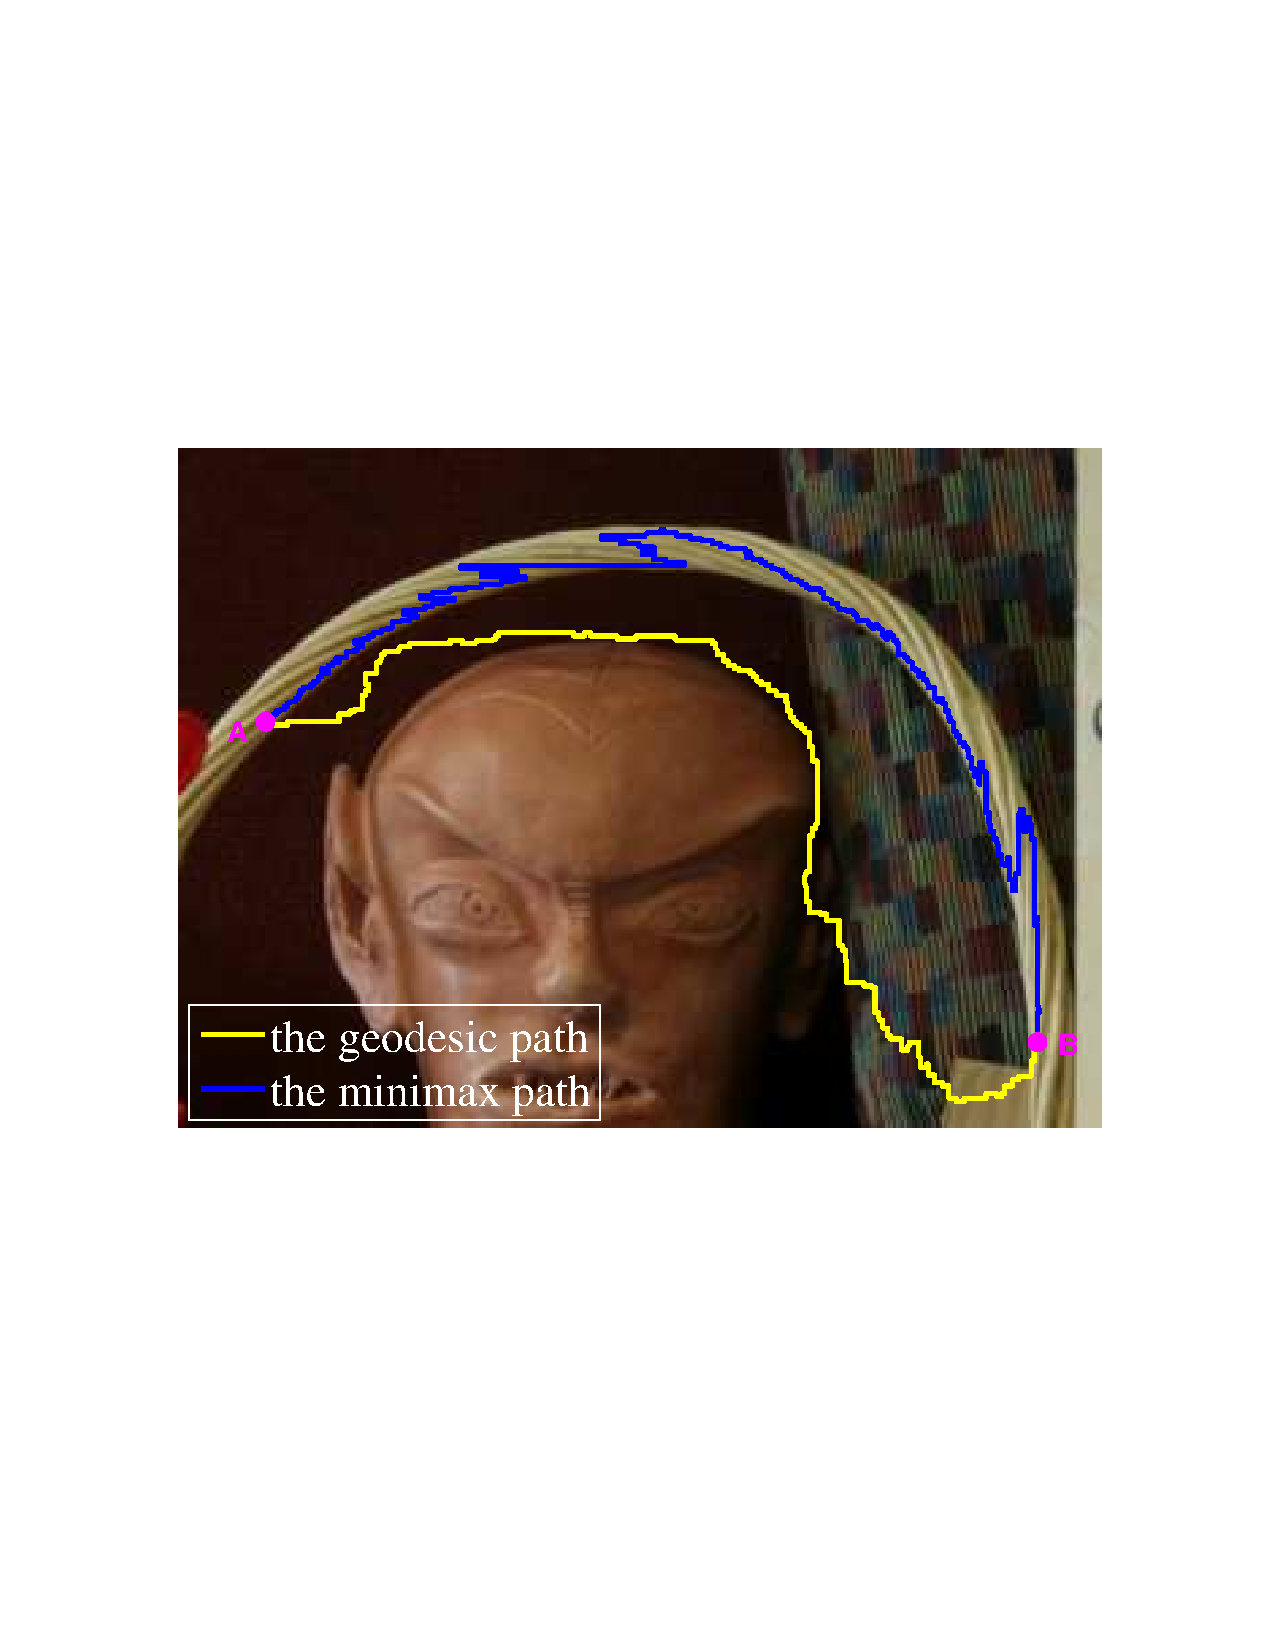
\includegraphics[width=\linewidth]{path.pdf}
    %\captionsetup{skip=1pt}
    %\caption{}
\end{subfigure}
\caption{ The comparison between the geodesic path and the minimax path. The figure shows that the geodesic chooses the crossing edges path which has a large jump at the color boundaries as almost the path is on the flatten area and the length on flatten area is nearly zeros whereas the minimax path is more sensitive to color edges and is able to follow the structure of guidance image.
}
\label{fig:minimax_path_comparison}
\end{figure}

Another advantage of minimax path is that we can efficiently extract all pairs minimax paths. Hu~\cite{Hu1961} proved that a path of the MST $T_G$ which connects distinct pairs of nodes $p,q$ is the minimax path of the $G$. Thus, all pairs minimax paths are recorded by the MST. In literature, the MST can be retrieved in linear time~\cite{Karger1995} for a single processor or in $O(\log n)$ time~\cite{Chong2001} for multiprocessors. Indeed, MST as a powerful tool which can capture the geometric structure of nature image has already been successfully used in image filtering~\cite{Stawiaski2009}, segmentation~\cite{Janakiraman2007} and cost aggregation~\cite{Yang2012}. In our application, MST guarantees that we can adaptively choose all the reliable seeds and will not interpolate depths across the boundary.

%
\begin{figure*}[t]
\centering
\begin{subfigure}[b]{0.2\linewidth}
    \centering
    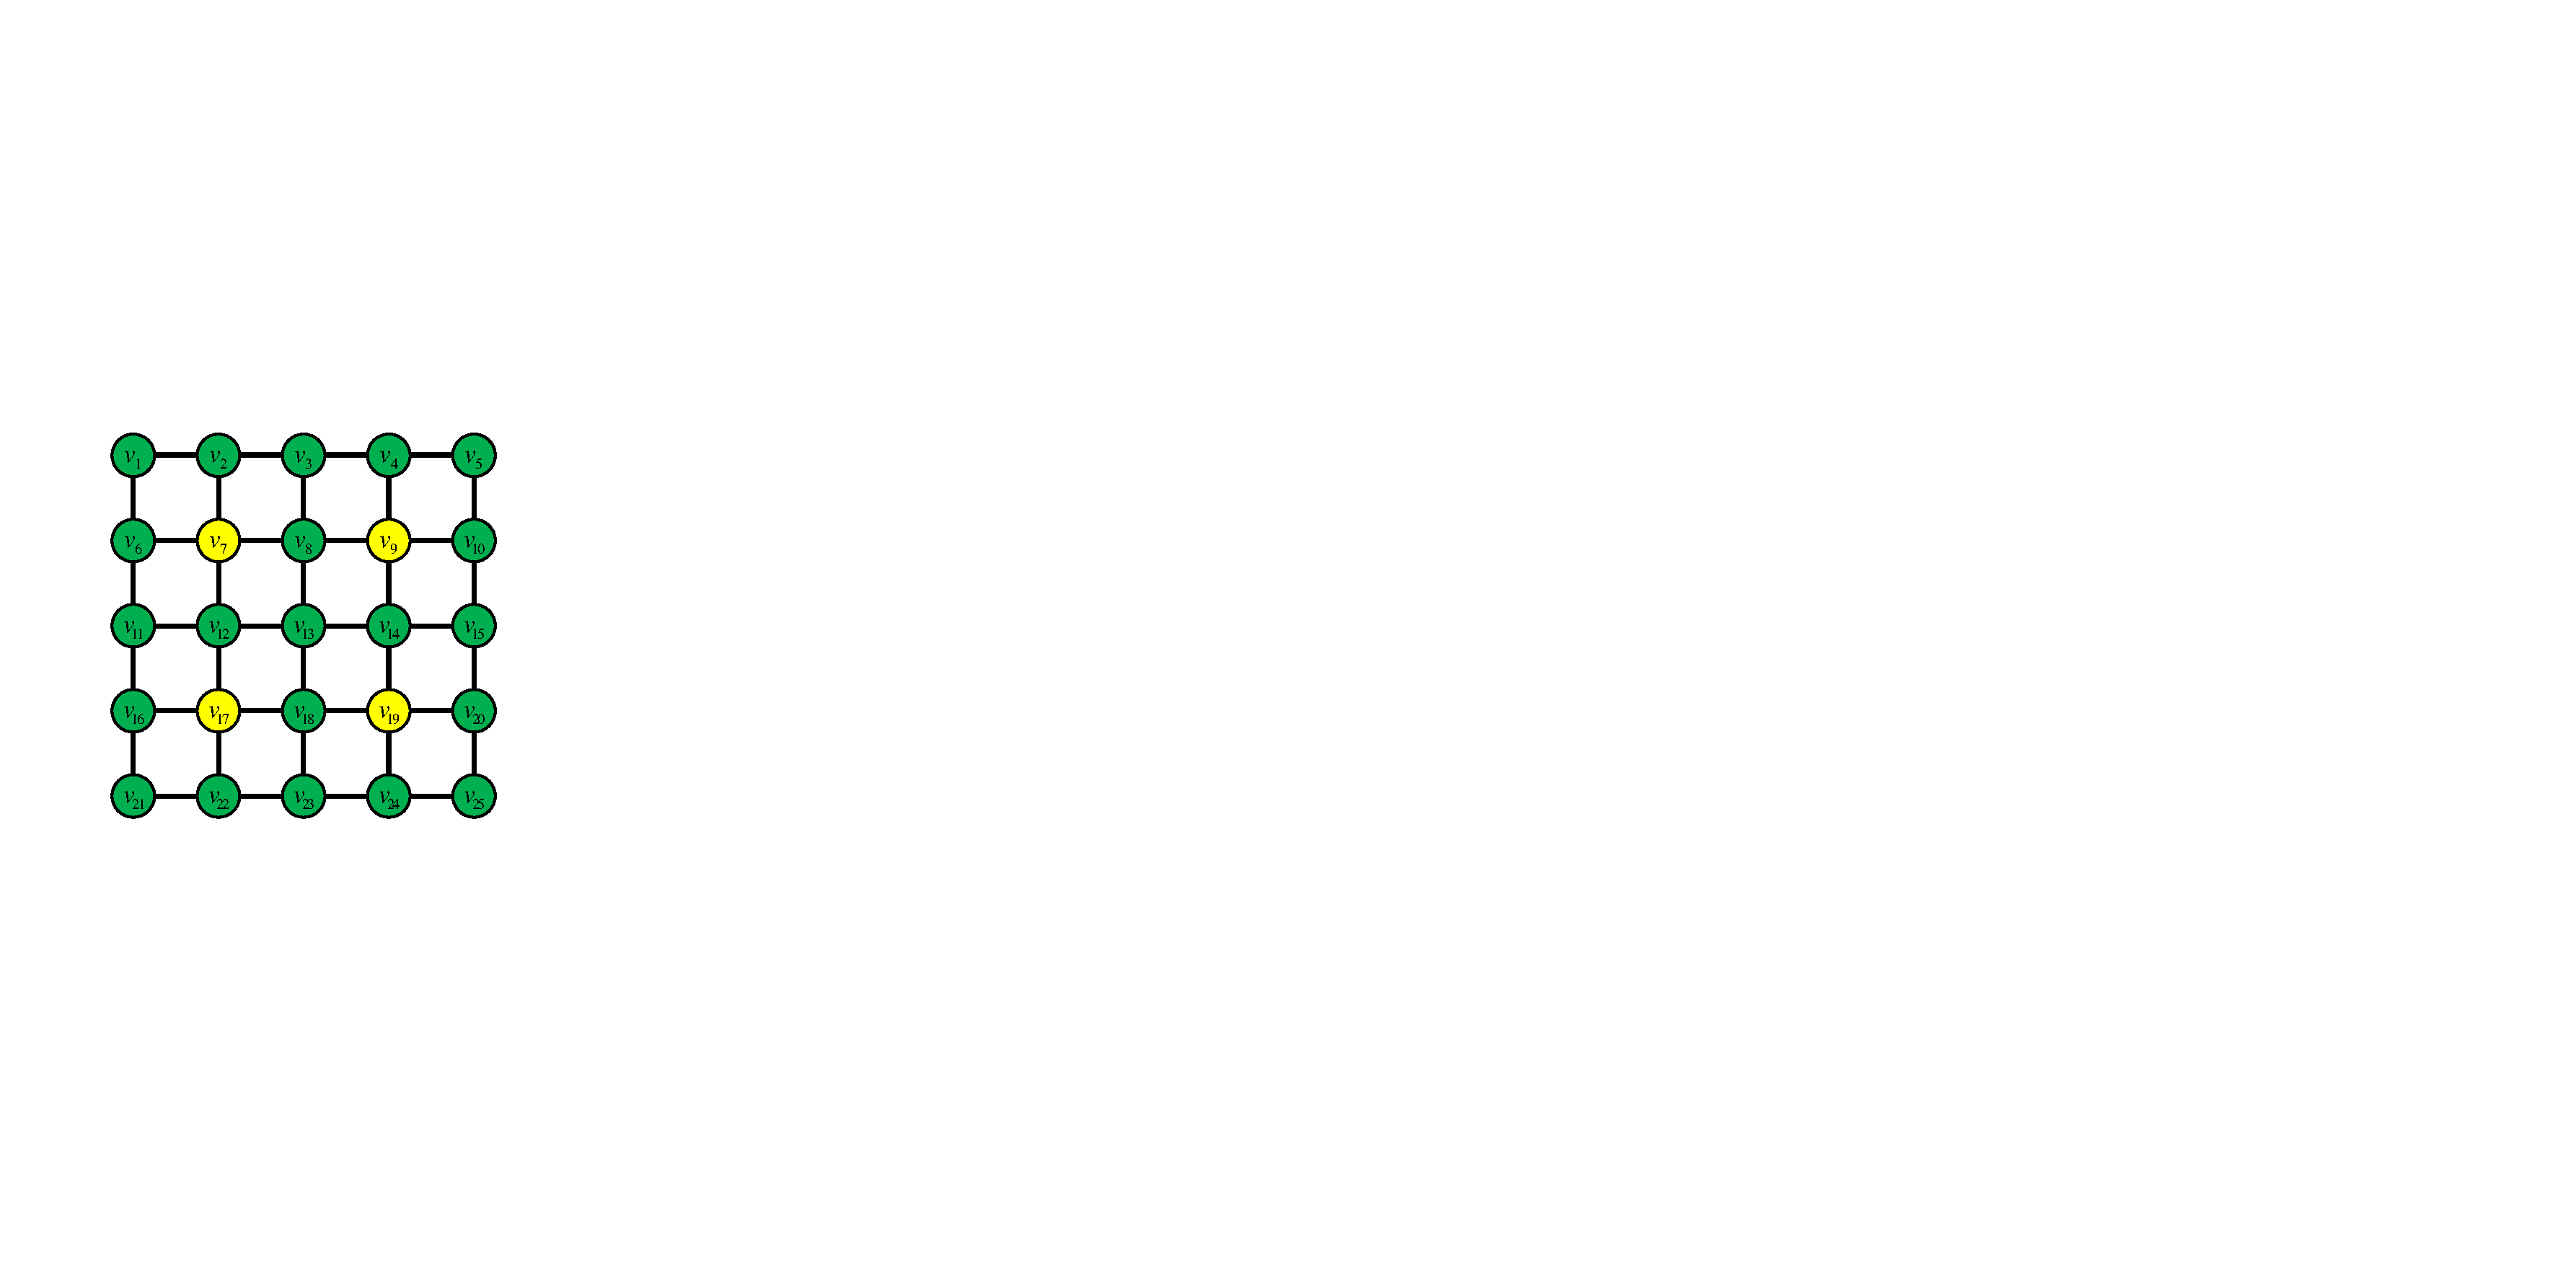
\includegraphics[width=\linewidth]{interpolation_tree_1.pdf}
    %\captionsetup{skip=1pt}
    \caption{AR}
    \label{fig:minimax_path:interpolation_tree_1}
\end{subfigure}
\hfill
\begin{subfigure}[b]{0.2\linewidth}
    \centering
    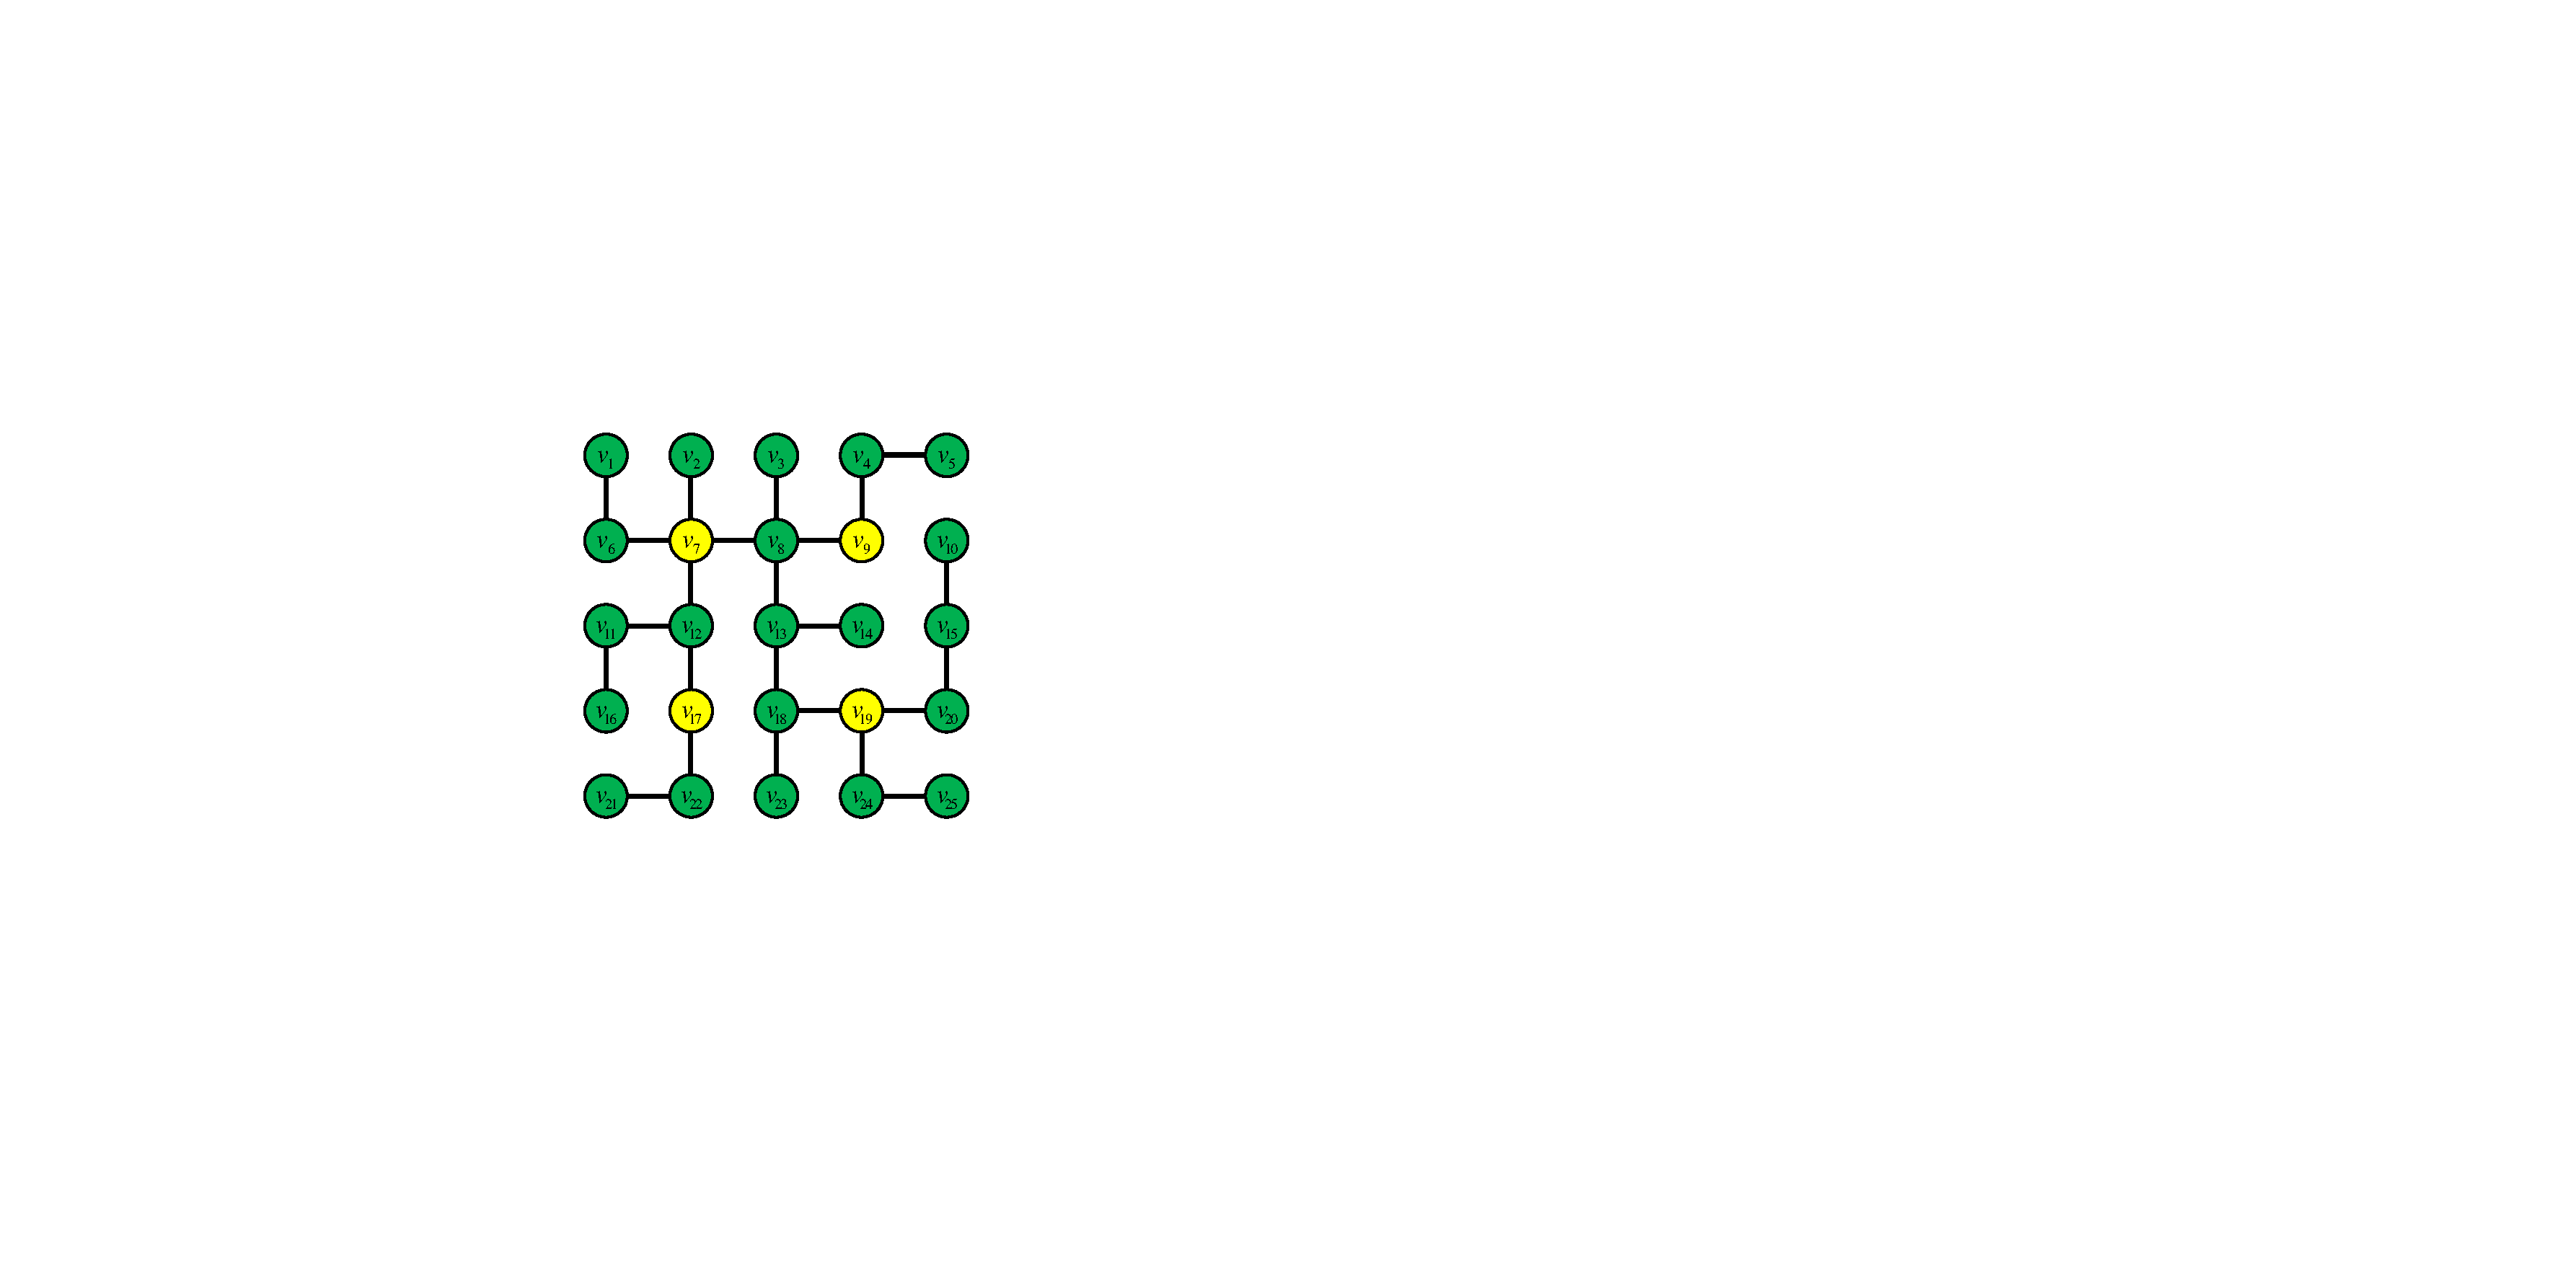
\includegraphics[width=\linewidth]{interpolation_tree_2.pdf}
    %\captionsetup{skip=1pt}
    \caption{}
    \label{fig:minimax_path:interpolation_tree_2}
\end{subfigure}\hfill
\begin{subfigure}[b]{0.2\linewidth}
    \centering
    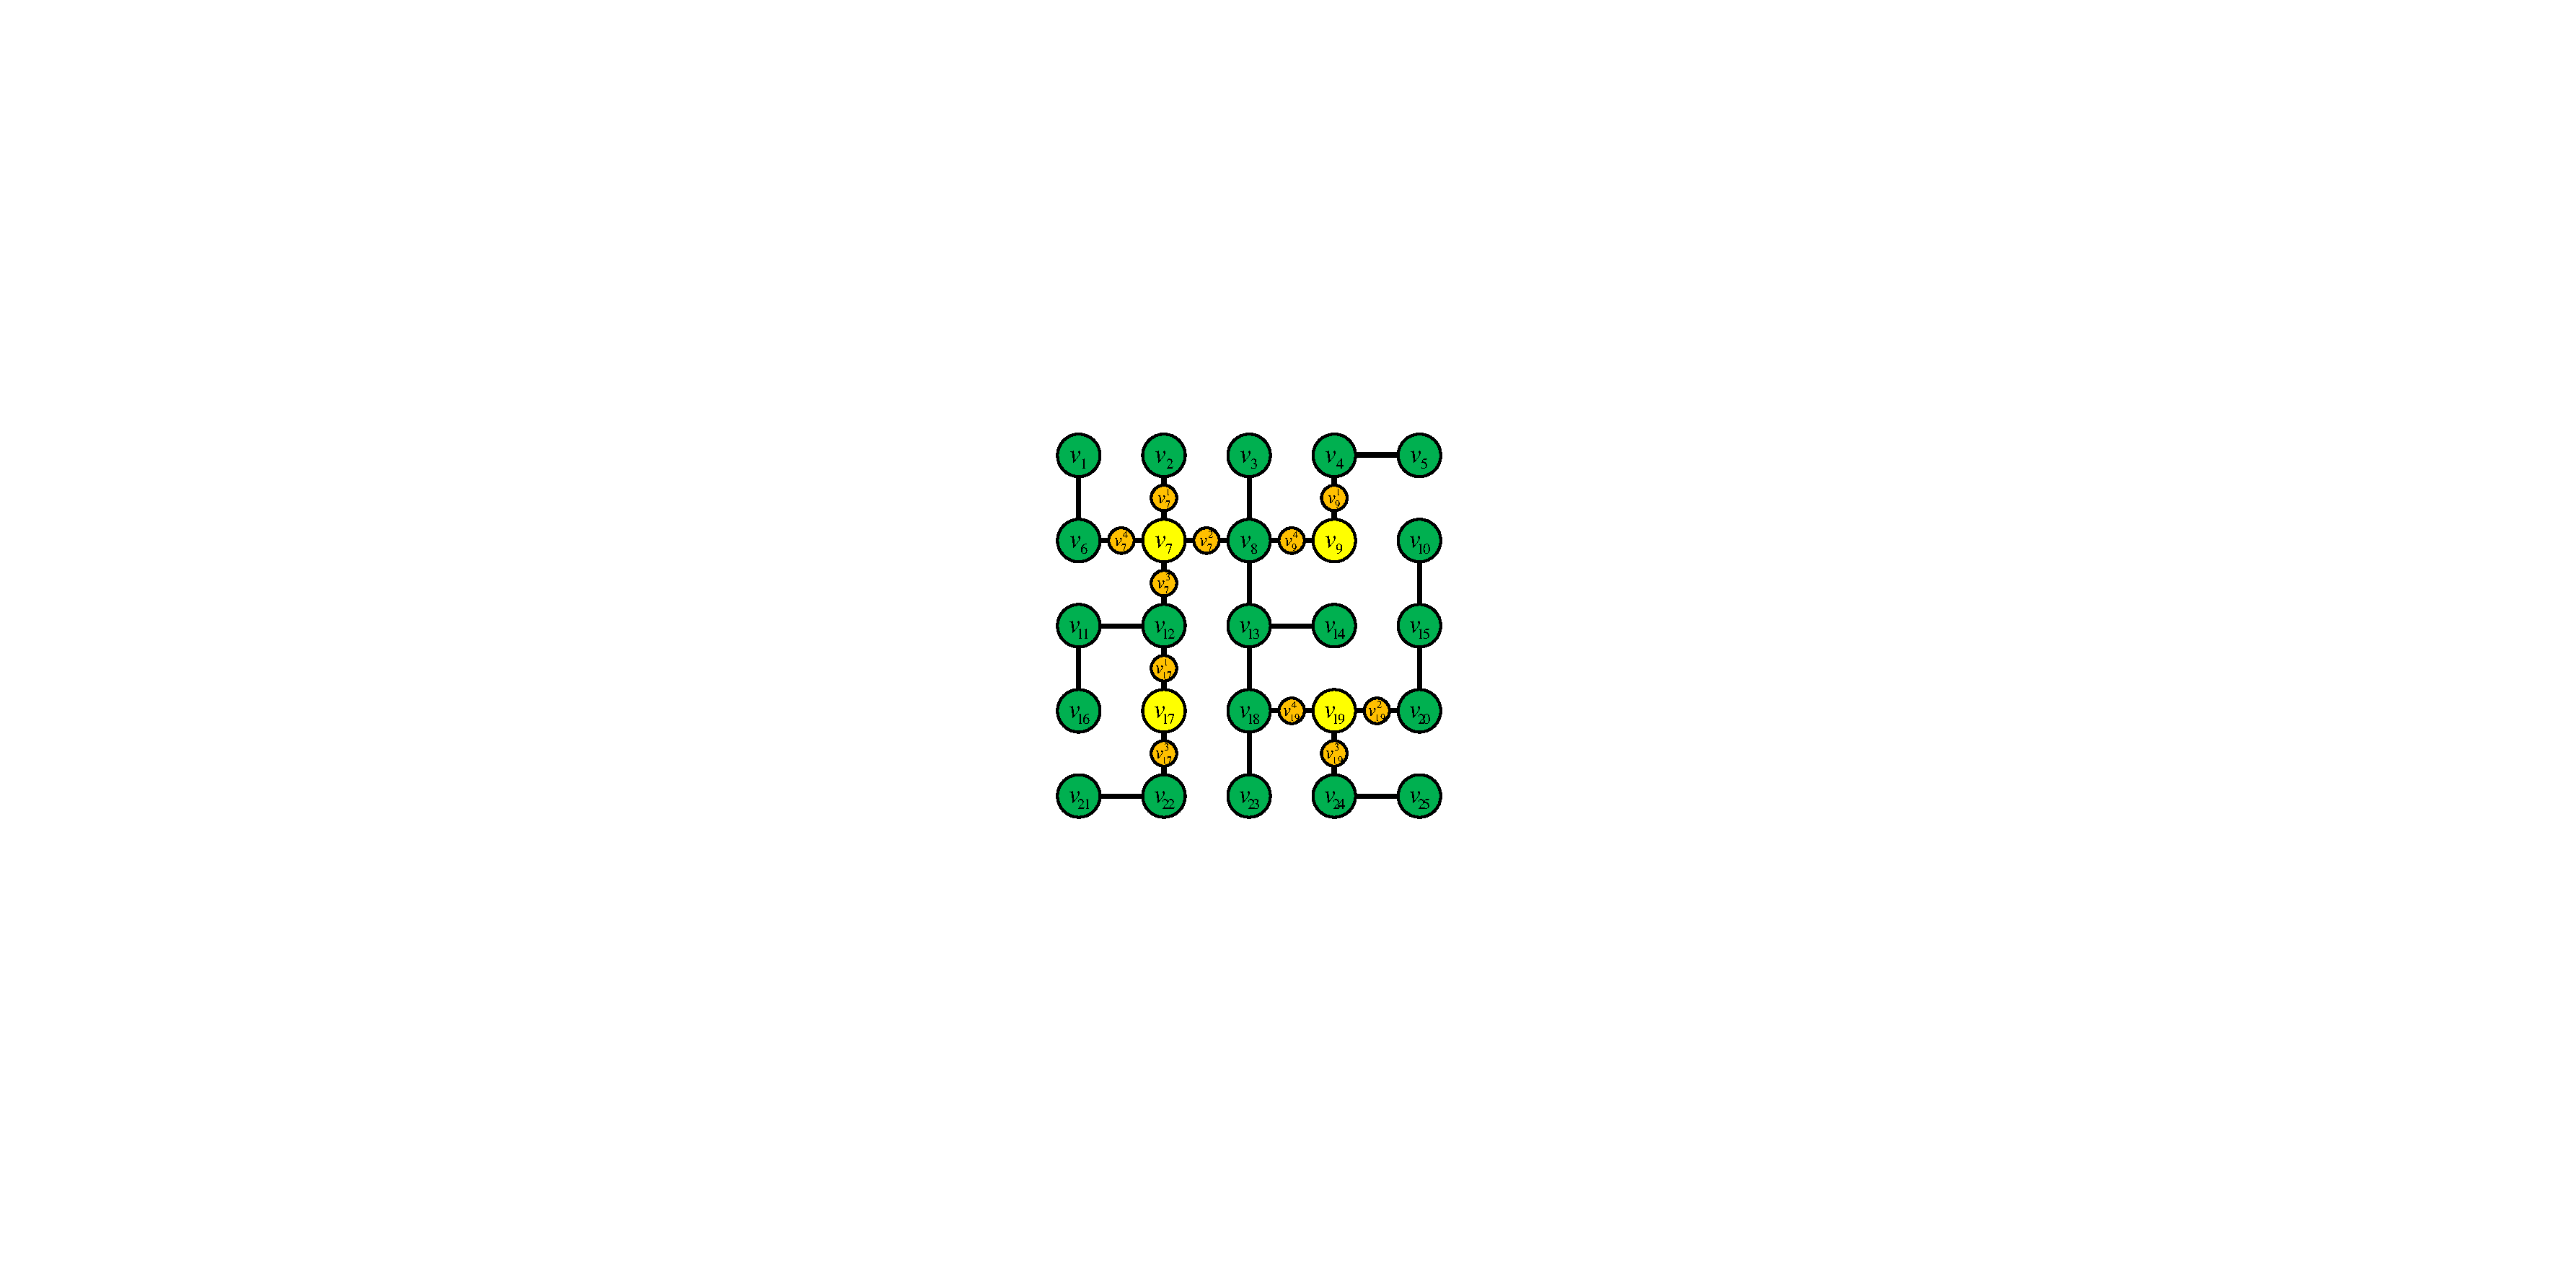
\includegraphics[width=\linewidth]{interpolation_tree_3.pdf}
    %\captionsetup{skip=1pt}
    \caption{}
    \label{fig:minimax_path:interpolation_tree_3}
\end{subfigure}\hfill
\begin{subfigure}[b]{0.2\linewidth}
    \centering
    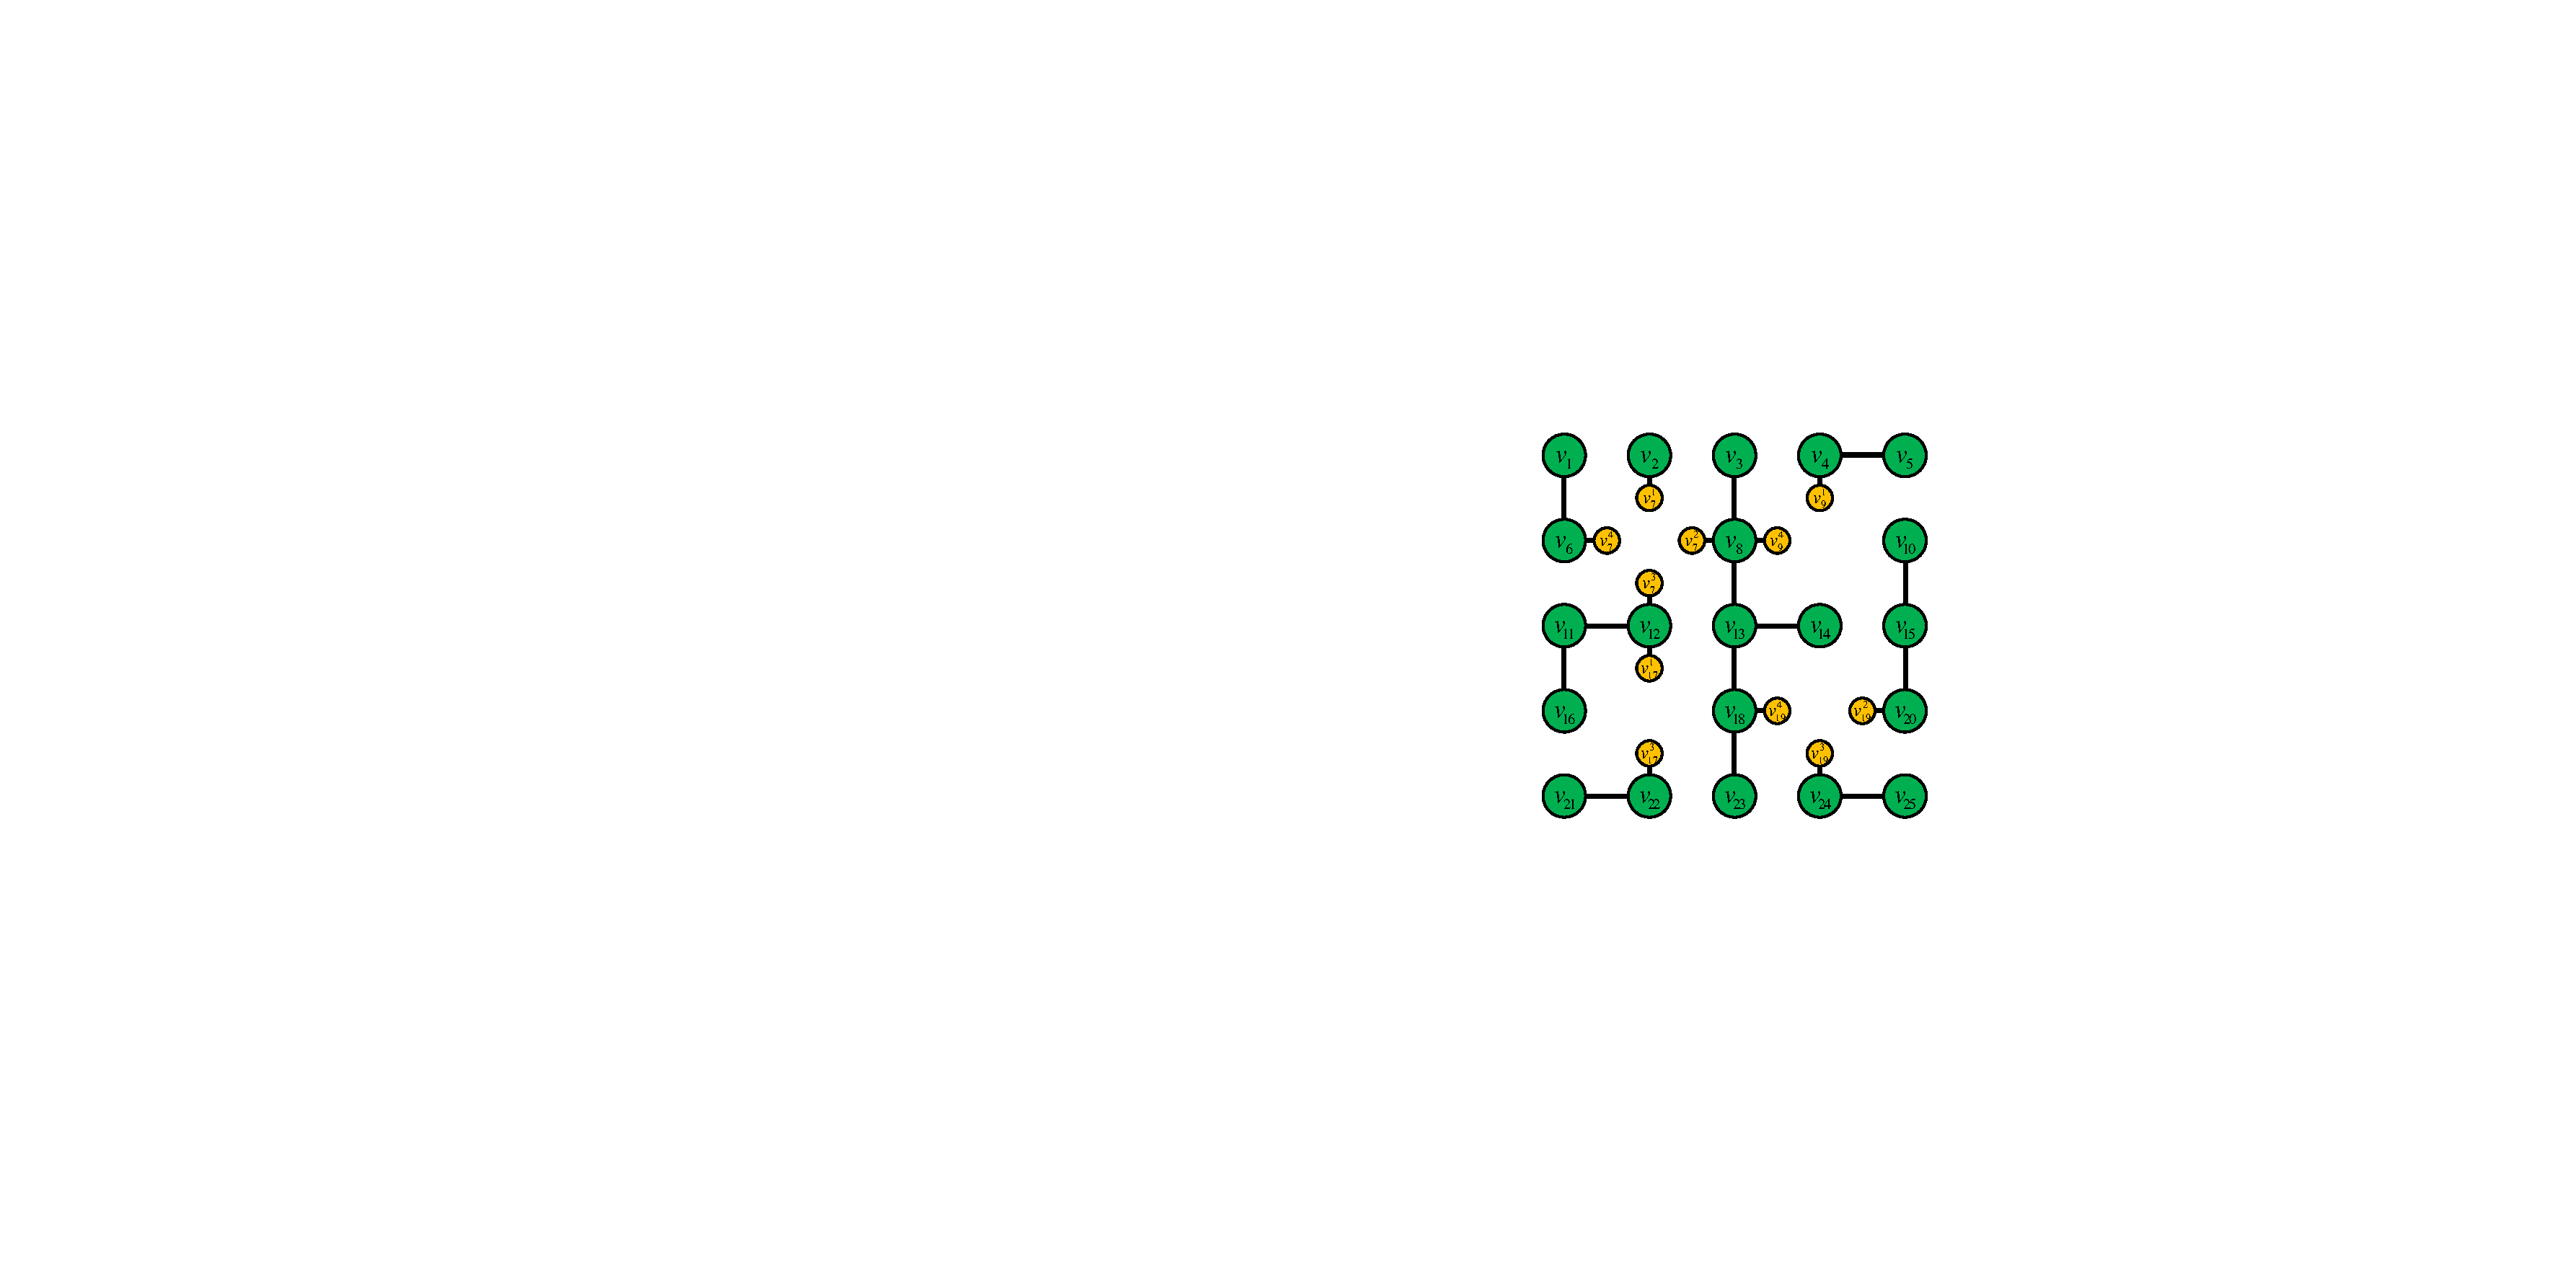
\includegraphics[width=\linewidth]{interpolation_tree_4.pdf}
    %\captionsetup{skip=1pt}
    \caption{}
    \label{fig:minimax_path:interpolation_tree_4}
\end{subfigure}
\caption{The minimax path illustration. (a) the graph representation $G$ of guidance image, where the green nodes are target pixels and yellow nodes denote seeds. (b) an MST of the graph $G$. The yellow seeds partition the green nodes into different parts. (c) the obtained interpolation tree by inserting orange auxiliary nodes into the MST. (d) the auxiliary nodes divide the interpolation tree into several parts by wiping off seeds.}
\label{fig:minimax_path}
\end{figure*}


At last, we notice that although there are lots of geometric aware distances such as the average-commute-time distance~\cite{Fouss2007} and the SoP covariance distance~\cite{Mantrach2010} in literature. However only the geodesic path and the minimax path are  discussed here. The reason is that all these geometric aware distances are extremely time consuming and thus they are not suited for depth interpolation in real time. In the depth upsampling literature, none of them are employed to upscale a low-resolution depth map. So we only compare the geodesic distance with the minimax path.




\subsection{A reliable seed choosing strategy}

An MST of the graph representation $G(V, E)$ of the depth map connects all points on the graph $G(V, E)$. The path linking two nodes along the MST is just the minimax path between them~\cite{Hu1961}. We can easily find that the seeds on the graph $G(V, E)$ separate the graph into $L$ different regions $\Omega_i$. So these seeds form the boundaries $B_i$ of these regions $\Omega_i$. For instance,  Fig~\ref{fig:minimax_path:interpolation_tree_1} illustrates a graph representation of a depth map, where the green nodes represent the target pixels and the yellow pixels denote the seeds.  Fig~\ref{fig:minimax_path:interpolation_tree_2} shows that an MST of the graph representation of the depth map connects all nodes together. Moreover, we can observe that the yellow seeds divide the green nodes into different parts and therefore form the boundaries of these partitions. In other words, for any two nodes in different regions, the path linking them along the MST must meet a yellow seed at least (\ie the minimax path from a non-boundary seed to any target pixel in $\Omega_i$ must pass through a boundary seed of $\Omega_i$). Since boundary points are the nearest seeds to the target pixels in the sense of the minimax distance, for each target pixel in the region $\Omega_i$,  using the depths of the boundary points $B_i$ to interpolate the depths of the target pixels in the region $\Omega_i$ is more reliable than using other seeds to interpolate
the missing depths. We call these boundary seeds $B_i$ as the reliable seeds of the target pixels in $\Omega_i$ and exclusively use their depths to interpolate the target pixels in $\Omega_i$.

%In other words, for any two nodes that are in different regions, the path links them along the MST must meet a yellow seed at lest.

The reliable seed choosing strategy has three major advantages. First, it automatically catches all reliable seeds for any target pixel and thus our interpolation algorithm can employ all reliable depth information to interpolate the depth of each target pixel. Second, it is not sensitive to the seed distribution and can be used for various seed distributions other than the uniform distribution taken by upsampling. Last but not  least, the strategy can be integrated into a linear time joint interpolation algorithm without extra cost.

\subsection{A linear complexity joint interpolation algorithm}
%
Our interpolation formula is expressed as Eq.~\eqref{eq:joint_mst}, which not just take the minimax distance as the similarity metric, but also employs our reliable seed choosing strategy to choose the interpolating seeds for each target pixel.
%
\begin{equation}
D(p) = \frac{ \sum\nolimits_{q \in B_i} {w^m_{p,q}D(q)} }{ {\sum\nolimits_{q \in B_i} {w^m_{p,q}}}} \quad p \in \Omega_i \setminus S \label{eq:joint_mst}
\end{equation}
%
where $w^m_{p,q} = \exp( - \frac{{d}(\pi_{{p},{q}}^m)}{\sigma_m})$ and $1 \leq i \leq L$.

The formula can be computed in a linear time by transforming the MST into an interpolation tree and updating depths along the interpolation tree $T$. Let $N(s)$ denote the neighborhood nodes which are linked to the seed $s$ by the MST. For each edge $e_{s, p}, p \in N(s)$, we insert an intermediate point $s_p$ into the middle of $s$ and $p$, as shown in Fig.\ref{fig:minimax_path:interpolation_tree_3}, and assign $d(e_{s_p, p}) = d(e_{s, p}), d(e_{s, s_p}) = \infty$. Here, all auxiliary points are denoted as $A$. We can observe from Fig.\ref{fig:minimax_path:interpolation_tree_4} that the interpolation tree $T$ is divided into $L$ subtrees $T_i$ by wiping off all seeds, and the depths of auxiliary nodes $\widetilde{B}_i = A \bigcap T_i$ determine the depths of the target pixels in the subtrees $T_i$. Then Eq.~\eqref{eq:joint_mst} can be rewritten as
%
\begin{equation}
D(p) = \frac{ \sum\nolimits_{q \in \widetilde{B}_i} {w^t_{p,q}D(q)} }{ {\sum\nolimits_{q \in \widetilde{B}_i} {w^t_{p,q}}}} \quad p \in T_i \setminus A, \ 1 \leq i \leq L \label{eq:joint_mst_re}
\end{equation}
%
where $w_{p,q} = \exp( - \frac{{d}(\pi^t_{{p},{q}})}{\sigma_m})$ and $\pi^t_{{p},{q}}$ is the path that connects $p$ to $q$ along the interpolation tree $T$.

    % Moreover, we denote all auxiliary points as $T$ for the convenience of following discussion.

In order to obtain the updating formulae with linear complexity, we put
$\widetilde C(q) = D(q)$, $\widetilde W(q) = 1$, for $q \in S$; $\widetilde C(q) = D(s)$, $\widetilde W(q) = 1$, for $q \in N(s), s \in S$; $\widetilde C(q) = 0$, $\widetilde W(q) = 0$, for a target pixel $q$, then Eq.~\eqref{eq:joint_mst_re} can be further transformed into following forms.
%
\begin{align}
&C(p) = \sum\nolimits_{q \in T} {w^t_{p,q} \widetilde C(q)} \ \ W(p) = \sum\nolimits_{q \in T} {w^t_{p,q} \widetilde W(q)} \label{eq:cost_coe} \\
&D(p) = C(p)/ W(p) \quad p \in T_i \setminus A, \ 1 \leq i \leq L \label{eq:depth}
\end{align}
%
In Eq.~\eqref{eq:cost_coe}, we replace $\widetilde{B}_i$ with $T$. Although the value of $C(p)$ and $W(p)$ for $p \in  T_i \setminus A$ receive supports from all other nodes on the interpolation tree $T$ according to Eq.~\eqref{eq:cost_coe}, the depths of target pixels in $T_i$ only depend on the depths of auxiliary nodes $\widetilde{B}_i$ as the length of the edge between the seed and its auxiliary points is set as infinity.


\begin{algorithm}[t]
\caption{Joint Interpolation Algorithm}
\begin{algorithmic}[1]
\REQUIRE
Graph $G=(V,E)$; Intermediate costs ${C^ \uparrow }(v)$, ${W^ \uparrow }(v)$;
Costs ${C }(v)$, ${W }(v)$;
\ENSURE
Depth map $D(v)$;
\FOR{each $v \in V$}
\IF{$v$ is a seed}
\STATE  ${C^ \uparrow }(v)={C }(v)=D(v)$; ${W^ \uparrow }(v)={W }(v)=1$;
\ELSE
\STATE  ${C^ \uparrow }(v)={C }(v)=0$;  ${W^ \uparrow }(v)={W }(v)=0$;
\ENDIF
\ENDFOR
\STATE  Retrieve an MST $T_G = (V, E')$ with $E' \subset E$ from G;
\STATE Assign each node $v \in V$ a breadth-first traversal order according to $T_G$;
\FOR { $i \in [\#T, \dots, 1]$ }
\IF{$P(v_i)$ is not a seed or  ${C^ \uparrow }(v_i)$, ${W^ \uparrow }(v_i)$ are 0}
\label{code:if1}
\STATE Update ${C^ \uparrow }(P(v_i))$, ${W^ \uparrow }(P(v_i))$ using Eq.~\eqref{eq:c_uparrow}~\eqref{eq:w_uparrow};
\ENDIF
\ENDFOR
\FOR { $i \in [1, \dots, \#T]$ }
\IF{$v_i$ is not a seed}
\label{code:if2}
\STATE Update ${C}(v_i)$, ${W}(v_i)$ using Eq.~\eqref{eq:c}~\eqref{eq:w};
\ENDIF
\ENDFOR
\STATE D(v) = C(v)/W(v) Eq.~\eqref{eq:depth};
\end{algorithmic}
\label{code:alg1}
\end{algorithm}

Yang~\cite{Yang2012} shows that the non-local cost aggregation form $C(p)$ and $W(p)$ which is defined on the tree can be efficiently figured out by traversing the tree structure of the interpolation tree $T$ in two sequential passes. Initially, we visit the nodes of $T_p$ using the breadth first traversal algorithm to assign each node $v_i$ an order $i$ based on the visit sequence with the property that if $v_i$ is the father of $v_j$, then $i \leqslant j$, where $ 1 \leqslant i,j \leqslant \#T_p$, $\#T_p$ denotes the nodes number of $T_p$. In the first pass, while the tree is traced from $v_{\#T_p}$ to $v_{1}$, ${C^ \uparrow }(v_i)$ and ${W^ \uparrow }(v_i)$ are not updated until all its children have been updated by the updating formulae~\eqref{eq:c_uparrow}~\eqref{eq:w_uparrow}.
%
\begin{align}
&{{C}^ \uparrow }(P(v_i)) = {{C}^ \uparrow }(P(v_i)) + {{w^t_{v_i,P(v_i)}}{{C}^ \uparrow }(v_i)} \label{eq:c_uparrow}\\
&{{W}^ \uparrow }(P(v_i)) = {{W}^ \uparrow }(P(v_i)) + {{w^t_{v_i,P(v_i)}}{{W}^ \uparrow }(v_i)} \label{eq:w_uparrow}
\end{align}
%
where ${C^ \uparrow }(v)$ and ${W^ \uparrow }(v)$ are initialized as $\widetilde{C}(v)$ and $\widetilde{W}(v)$, $P(v)$ records the father of node $v$, both ${C^ \uparrow }(v)$ and ${W^ \uparrow }(v)$ are the intermediate aggravated results. In the second pass, we employ the updating formulae~\eqref{eq:c}~\eqref{eq:w} to renew $C(v)$ and $W(v)$ when the tree is traversed from $v_1$ to $v_{\#T_p}$. At last, we use Eq.~\eqref{eq:depth} to estimate final interpolation depths.
%
\begin{align}
& C(v_i) = {w^t_{P(v_i),v_i}}{\widetilde{C}({P(v_i)})} + (1 - {w^{t^2}_{v_i,P(v_i)}}){C^ \uparrow }(v_i) \label{eq:c}\\
& W(v_i) = {w^t_{P(v_i),v_i}}{\widetilde{W}({P(v_i)})} + (1 - {w^{t^2}_{v_i,P(v_i)}}){W^ \uparrow }(v_i) \label{eq:w}
\end{align}
%

At last, removing all auxiliary points $s_p$ from final results, we can obtain the interpolation results. Note that since $d(e_{s_p, s})$ is infinity, no points can contribute its depth to the seed $s$ through the edge $e_{s_p, s}$. We thus are able to keep the depths of seeds unchanged. Conversely, the depths of seeds would also not propagate its depth to target pixels. This is an undesirable situation. To solve the problem, we assign the depths of seeds to the auxiliary points $s_p$ and employ $s_p$ as proxies to propagate the depths of seeds to target pixels in the same regions. This is the reason why we introduce auxiliary points at first and get rid of them at last.

\subsection{Refinement of the joint interpolation algorithm}


%
\begin{table}[t]
\centering
\begin{tabular}{|l|l|l|l|l|}
\hline
     & MST1 & MST2 & MST3 & MST4 \\ \hline
SSIM &  0.987    &   0.991   &  0.989    &  0.994    \\ \hline
\end{tabular}
\caption{The similarity measurements for the interpolation results produced by different MSTs. The SSIM indices are calculated from an interpolation reference image and four comparison interpolation images, where both the reference image and four comparison images are produced by different MSTs.}
\label{tab:SSIM}
\end{table}
%

\begin{figure*}[t]
\centering
\begin{subfigure}[b]{0.35\linewidth}
     %% label for first subfigure
    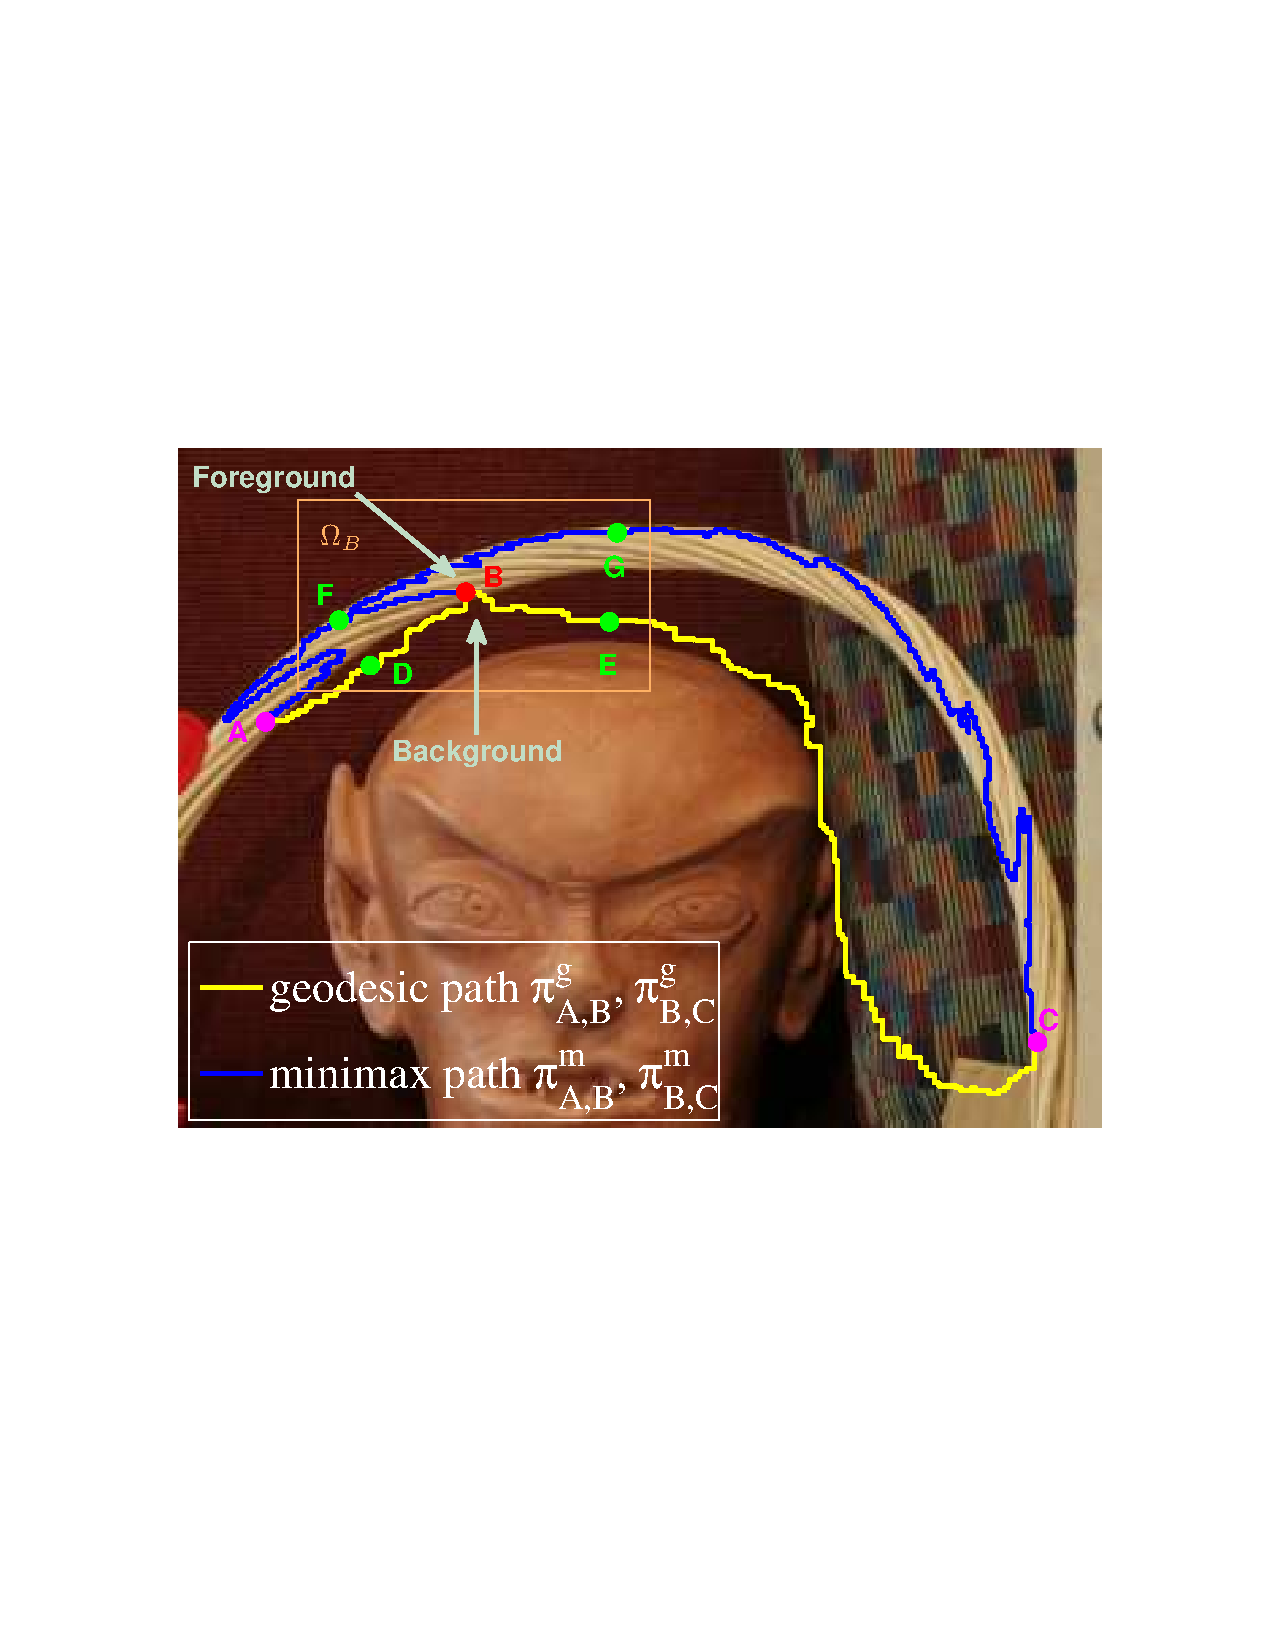
\includegraphics[width=\linewidth]{path1.pdf}
    \caption{}
    \label{fig:path:path}
\end{subfigure}%
%-------------------------------
\begin{subfigure}[b]{0.4\linewidth}
    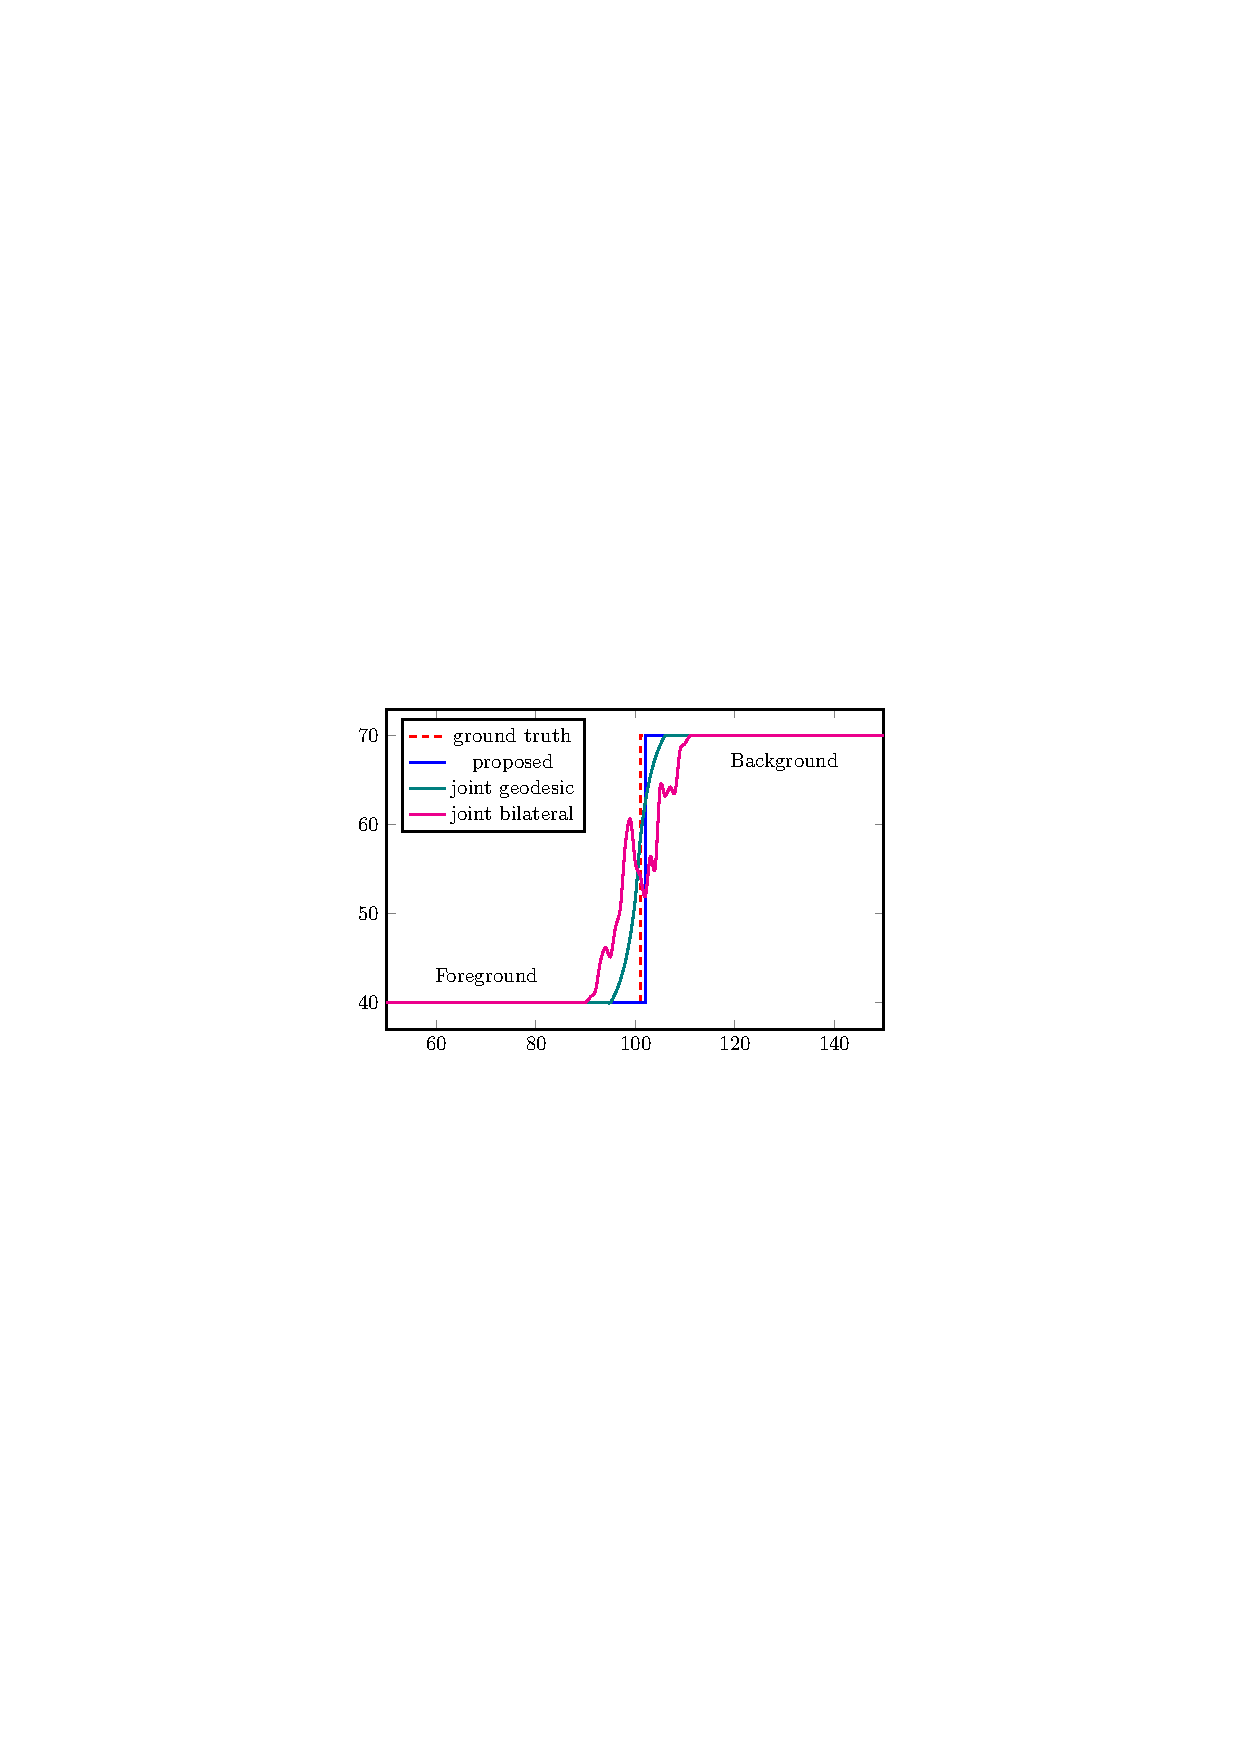
\includegraphics[width=\linewidth]{JUE.pdf}
    % \captionsetup{skip=14pt}
    \caption{}
    \label{fig:path:edge}
\end{subfigure}
%\begin{subfigure}[b]{0.01\linewidth}
%    \captionsetup{skip=35pt}
%    \caption{}
%    \label{fig:path:edge} %% label for first subfigure
%\end{subfigure}
\caption{\textbf{Comparison among joint bilateral, joint geodesic and our upsampling methods.} (a) geodesic paths and minimax paths between A, B and B, C, where B is the target point, D, E, F and G are the seeds, D and E, F and G are  on the geodesic paths and minimax paths, respectively. (b) The upsampled depth profiles of joint bilateral, joint geodesic and our upsampling methods.}
\label{fig:path}
%\vspace{-0.5cm}
\end{figure*}


The linear complexity joint interpolation algorithm stated above is not the most efficient interpolation algorithm yet as it involves the operation of interpolating nodes into a predefined MST and removing them from final results. Supposing that the redundant operation could be eliminated, the algorithm will become more compact. Through an in-depth analysis, we can discover that the auxiliary points $s_p$ are only used to prohibit the depths diffusion between different parts $B_i$ which are segmented by the seeds $S$ along the MST. The function of auxiliary points can be replaced by introducing if statement to judge whether the algorithm propagates depth information across boundaries. Specifically, in the bottom to top pass, we check whether the point $P(v_i)$ is a seed. If it is not a seed, we use Eq.~\eqref{eq:c_uparrow} and Eq.~\eqref{eq:w_uparrow} to update the values of ${{C}^ \uparrow }(P(v_i))$ and ${{W}^ \uparrow }(P(v_i))$. Otherwise, we keep them unchanged. Similarly, in the up to down pass, we check whether the point $v_i$ is a seed. If it is not a seed, we use Eq.~\eqref{eq:c} and Eq.~\eqref{eq:w} to update the values of $C(v_i)$ and $W(v_i)$. Otherwise, we also keep them unchanged. In this paper, we adopt the updating strategy to remove the unnecessary auxiliary points and report the refined interpolation algorithm in Alg~\ref{code:alg1}.

At last, we discuss an implementation detail for people who are interested in it. As is known to all, the MST is not unique for a graph. In this situation, we can choose more than one MST to perform interpolation. People maybe wonder what would happen if there are more than only one MST and how to choose an appropriate MST. Frankly speaking, Alg~\ref{code:alg1} does not tell us how to determine an MST because it is not important. More clearly, our algorithm is rather robust for different MSTs. To prove this, we randomly select five different MSTs and choose the interpolation result of an MST as the reference image. After that, we compare the comparison interpolation results (\ie interpolation results of the other MSTs) with the reference and quantify the similarity. Here, we prefer the structural similarity (SSIM) index~\cite{Wang_TIP_2004} to measure the affinity between two images. For SSIM index, one is only reachable in the case of two identical sets of data, and zero means two images are completely different. The SSIM data in Tab~\ref{tab:SSIM} demonstrates that the similarity between the comparison interpolation results and the reference image. It is easy to verify that the interpolation results for different MSTs are nearly same.


\subsection{An analysis of the computational complexity}

The computational complexity of our method is consisted of two parts: the cost of extracting an MST from the graph representation $G$ of the guidance image $I$ and the cost of updating Eq.~\eqref{eq:c_uparrow}~\eqref{eq:w_uparrow}~\eqref{eq:c}~\eqref{eq:w}. In Eq.~\eqref{eq:c_uparrow}~\eqref{eq:w_uparrow}~\eqref{eq:c}~\eqref{eq:w}, ${w^t_{P(v_i),v_i}}$ only depends on the edge weights of the interpolation tree $T$ and can be pre-computed in linear complexity. Thus, only a total of 6 addition/subtraction operations and 7 multiplication/division operations are required for each node. Hence we can complete the interpolation task with $O(n)$ complexity disregarding the number $K$ of reliable seeds.

For extracting an MST from a graph, Karger~\etal~\cite{Karger1995} presented a linear time randomized algorithm to extract an MST from a graph. With a linear number of processors, the parallel algorithm~\cite{Chong2001} for the minimum spanning tree problem can solve the problem in $O(\log n)$ time. Overall, we conclude that the overall complexity of our algorithm is $O(n)$.


\section{Experiments}
\label{sec:experiments}



We implement our algorithm using Matlab and compare it with state-of-the-art methods on a desktop computer with 4 GB memory. At first, we will disclose why our method can achieve the best results in terms of accuracy and efficiency by performing an in-deep investigation on the difference between our algorithm and other depth upsampling methods. After that, the parameter sensitivity and computational analysis of our algorithm are offered. Finally, we exhibit the interpolation results of real world data to test the interpolation ability of our method.

\subsection{An in-deep investigation}

\begin{table*}[!t]%\fontsize{8pt}{0.5\baselineskip}\selectfont
%\vspace{-0.5cm}
\centering

\begin{tabularx}{\textwidth}{@{}|l|l|YYYY|YYYY|YYYY|@{}}
\hline
\multicolumn{2}{|c|}{  } & \multicolumn{4}{c|}{ Art} & \multicolumn{4}{c|}{ Book} & \multicolumn{4}{c|}{ Moebius} \\
%\cline{3-14}
\multicolumn{2}{|c|}{  } & 2X & 4X & 8X & 16X  & 2X & 4X & 8X & 16X  & 2X & 4X & 8X & 16X \\
\hline
\cline{3-14}
\multirow{2}{*}{AR~\cite{YangJingyu2012}}
                            & DISC
                            & 0.15 & 0.24 & 0.32 & 0.41
                            & 0.12 & 0.23 & 0.34 & 0.39
                            & 0.12 & 0.20 & 0.29 & 0.33 \\
                            & CONT
                            & 0.03 & 0.06 & 0.10 & 0.17
                            & 0.03 & 0.05 & 0.10 & 0.19
                            & 0.02 & 0.04 & 0.07 & 0.14 \\
\hline
%\multirow{2}{*}{BF~\cite{YangQingxiong2007}}
%                            & DISC
%                            & 0.19 & 0.29 & 0.42 & 0.47
%                            & 0.15 & 0.26 & 0.45 & 0.49
%                            & 0.20 & 0.26 & 0.35 & 0.47 \\
%                            & CONT
%                            & 0.05 & 0.12 & 0.10 & 0.12
%                            & 0.07 & 0.07 & 0.13 & 0.16
%                            & 0.14 & 0.12 & 0.12 & 0.13 \\
%\hline
\multirow{2}{*}{NLA~\cite{Yang2012}}
                            & DISC
                            & 0.17 & 0.27 & 0.39 & 0.48
                            & 0.22 & 0.33 & 0.41 & 0.49
                            & 0.16 & 0.24 & 0.33 & 0.48 \\
                            & CONT
                            & 0.01 & 0.04 & 0.07 & 0.12
                            & 0.02 & 0.04 & 0.08 & 0.18
                            & 0.01 & 0.03 & 0.05 & 0.10 \\
\hline
\multirow{2}{*}{JBL~\cite{Kopf2007}}
                            & DISC
                            & 0.16 & 0.24 & 0.39 & 0.49
                            & 0.19 & 0.27 & 0.41 & 0.49
                            & 0.16 & 0.23 & 0.35 & 0.48 \\
                            & CONT
                            & 0.01 & 0.03 & 0.06 & 0.12
                            & 0.01 & 0.02 & 0.05 & 0.16
                            & 0.01 & 0.02 & 0.04 & 0.10 \\
\hline
\multirow{2}{*}{JG~\cite{Liu2013}}
                            & DISC
                            & 0.11 & 0.19 & 0.30 & 0.36
                            & 0.06 & 0.18 & 0.35 & 0.43
                            & 0.10 & 0.20 & 0.24 & 0.34 \\
                            & CONT
                            & 0.03 & 0.05 & 0.08 & 0.12
                            & 0.03 & 0.05 & 0.09 & 0.17
                            & 0.02 & 0.04 & 0.06 & 0.12 \\
\hline
\multirow{2}{*}{LF~\cite{Kang_ET_2014}}
                            & DISC
                            & 0.09 & 0.17 & 0.26 & 0.31
                            & 0.05 & 0.14 & 0.20 & 0.33
                            & 0.08 & 0.17 & 0.20 & 0.32 \\
                            & CONT
                            & 0.02 & 0.04 & 0.08 & 0.12
                            & 0.02 & 0.05 & 0.09 & 0.15
                            & 0.01 & 0.02 & 0.06 & 0.10 \\
\hline
\multirow{2}{*}{ST~\cite{Choi_TIP_2014}}
                            & DISC
                            & 0.07 & 0.12 & 0.21 & 0.27
                            & 0.03 & 0.10 & 0.12 & 0.21
                            & 0.06 & 0.12 & 0.16 & 0.27 \\
                            & CONT
                            & 0.01 & 0.04 & 0.07 & 0.12
                            & 0.01 & 0.04 & 0.08 & 0.14
                            & 0.01 & 0.02 & 0.05 & 0.11 \\
\hline
\multirow{2}{*}{Ours }
                            & DISC
                            & 0.04 & 0.09 & 0.16 & 0.22
                            & 0.02 & 0.06 & 0.09 & 0.15
                            & 0.04 & 0.09 & 0.14 & 0.21 \\
                            & CONT
                            & 0.01 & 0.03 & 0.07 & 0.12
                            & 0.01 & 0.04 & 0.08 & 0.13
                            & 0.01 & 0.02 & 0.05 & 0.10 \\
\hline
\end{tabularx}
\caption{\textbf{PBP quantitative comparison.} We compare the proposed algorithm with state-of-the-art methods on the Middlebury dataset using percentage of bad matching pixels (PBP)~\cite{Scharstein2002}, where the disparity error tolerance is $1$. DISC denotes the PBP index at discontinuous regions and CONT stands for the PBP index at continuous areas.}
\label{tab:PBP}
\end{table*}

\begin{table*}[!t]%\fontsize{8pt}{0.5\baselineskip}\selectfont
%\vspace{-0.5cm}
\centering

\begin{tabularx}{\textwidth}{@{}|l|l|YYYY|YYYY|YYYY|@{}}
\hline
\multicolumn{2}{|c|}{  } & \multicolumn{4}{c|}{ Art} & \multicolumn{4}{c|}{ Book} & \multicolumn{4}{c|}{ Moebius} \\
%\cline{3-14}
\multicolumn{2}{|c|}{  } & 2X & 4X & 8X & 16X  & 2X & 4X & 8X & 16X  & 2X & 4X & 8X & 16X \\
\hline
\cline{3-14}
\multirow{2}{*}{AR~\cite{YangJingyu2012}}
                            & DISC
                            & 25.94 & 24.08 & 23.42 & 19.54
                            & 33.93 & 32.19 & 29.11 & 25.43
                            & 35.15 & 32.78 & 30.06 & 26.74 \\
                            & CONT
                            & 47.88 & 46.28 & 44.98 & 41.38
                            & 56.27 & 53.96 & 51.04 & 48.31
                            & 57.03 & 54.27 & 52.76 & 50.12 \\
\hline
%\multirow{2}{*}{BF~\cite{YangQingxiong2007}}
%                            & DISC
%                            & 44.54 & 44.01 & 43.30 & 38.42
%                            & 0.15 & 0.26 & 0.45 & 0.49
%                            & 0.20 & 0.26 & 0.35 & 0.47 \\
%                            & CONT
%                            & 0.05 & 0.12 & 0.10 & 0.12
%                            & 0.07 & 0.07 & 0.13 & 0.16
%                            & 0.14 & 0.12 & 0.12 & 0.13 \\
%\hline
\multirow{2}{*}{NLA~\cite{Yang2012}}
                            & DISC
                            & 24.72 & 23.22 & 21.41 & 19.47
                            & 33.14 & 30.94 & 26.61 & 23.04
                            & 32.02 & 29.96 & 27.48 & 24.54 \\
                            & CONT
                            & 46.94 & 46.01 & 44.69 & 40.38
                            & 56.03 & 52.97 & 51.04 & 47.31
                            & 56.81 & 53.92 & 52.98 & 49.47 \\
\hline
\multirow{2}{*}{JBL~\cite{Kopf2007}}
                            & DISC
                            & 24.30 & 23.03 & 21.06 & 19.12
                            & 32.74 & 30.11 & 26.05 & 23.16
                            & 31.92 & 29.02 & 27.48 & 24.05 \\
                            & CONT
                            & 47.54 & 46.01 & 43.30 & 41.42
                            & 55.56 & 53.11 & 50.89 & 47.21
                            & 56.18 & 53.97 & 51.64 & 49.71 \\
\hline
\multirow{2}{*}{JG~\cite{Liu2013}}
                            & DISC
                            & 25.72 & 23.89 & 22.76 & 18.83
                            & 33.13 & 31.47 & 28.31 & 25.03
                            & 34.98 & 32.64 & 29.69 & 27.63 \\
                            & CONT
                            & 46.92 & 45.89 & 44.35 & 40.83
                            & 55.18 & 53.23 & 51.76 & 49.21
                            & 57.22 & 54.16 & 52.64 & 49.64 \\
\hline
\multirow{2}{*}{LF~\cite{Kang_ET_2014}}
                            & DISC
                            & 24.29 & 22.79 & 22.21 & 18.95
                            & 32.73 & 30.17 & 27.95 & 26.46
                            & 33.50 & 31.88 & 29.00 & 27.02 \\
                            & CONT
                            & 46.77 & 45.92 & 44.24 & 40.99
                            & 55.92 & 53.34 & 51.65 & 48.47
                            & 56.96 & 54.47 & 51.49 & 50.40 \\
\hline
\multirow{2}{*}{ST~\cite{Choi_TIP_2014}}
                            & DISC
                            & 26.07 & 24.21 & 23.22 & 19.21
                            & 34.32 & 32.06 & 29.74 & 26.61
                            & 35.11 & 33.24 & 30.29 & 28.73 \\
                            & CONT
                            & 47.02 & 46.19 & 45.05 & 41.42
                            & 56.02 & 53.34 & 51.60 & 48.91
                            & 57.63 & 54.74 & 52.45 & 50.17 \\
\hline
\multirow{2}{*}{Ours }
                            & DISC
                            & 26.87 & 25.22 & 24.01 & 20.74
                            & 35.02 & 32.96 & 30.48 & 27.54
                            & 36.14 & 33.94 & 31.61 & 29.22 \\
                            & CONT
                            & 47.12 & 46.29 & 45.01 & 41.54
                            & 56.60 & 53.42 & 51.60 & 49.01
                            & 57.81 & 54.92 & 52.03 & 50.47 \\
\hline
\end{tabularx}
\caption{\textbf{PSNR quantitative comparison.} We compare the proposed algorithm with state-of-the-art methods on the Middlebury dataset using the peak signal-to-noise ratio (PSNR)~\cite{Huynh_EL_2008}. DISC denotes the PSNR index at discontinuous regions and CONT stands for the PSNR index at continuous areas.}
\label{tab:PSNR}
\end{table*}

%\begin{table*}[!t]%\fontsize{8pt}{0.5\baselineskip}\selectfont
%%\vspace{-0.5cm}
%\centering
%
%\begin{tabularx}{\textwidth}{@{}|l|l|YYYY|YYYY|YYYY|@{}}
%\hline
%\multicolumn{2}{|c|}{  } & \multicolumn{4}{c|}{ Art} & \multicolumn{4}{c|}{ Book} & \multicolumn{4}{c|}{ Moebius} \\
%%\cline{3-14}
%\multicolumn{2}{|c|}{  } & 2X & 4X & 8X & 16X  & 2X & 4X & 8X & 16X  & 2X & 4X & 8X & 16X \\
%\hline
%\cline{3-14}
%\multirow{2}{*}{AR~\cite{YangJingyu2012}}
%                            & DISC
%                            & 0.15 & 0.24 & 0.32 & 0.41
%                            & 0.12 & 0.23 & 0.34 & 0.39
%                            & 0.12 & 0.20 & 0.29 & 0.33 \\
%                            & CONT
%                            & 0.03 & 0.06 & 0.10 & 0.17
%                            & 0.03 & 0.05 & 0.10 & 0.19
%                            & 0.02 & 0.04 & 0.07 & 0.14 \\
%\hline
%%\multirow{2}{*}{BF~\cite{YangQingxiong2007}}
%%                            & DISC
%%                            & 0.19 & 0.29 & 0.42 & 0.47
%%                            & 0.15 & 0.26 & 0.45 & 0.49
%%                            & 0.20 & 0.26 & 0.35 & 0.47 \\
%%                            & CONT
%%                            & 0.05 & 0.12 & 0.10 & 0.12
%%                            & 0.07 & 0.07 & 0.13 & 0.16
%%                            & 0.14 & 0.12 & 0.12 & 0.13 \\
%%\hline
%\multirow{2}{*}{NLA~\cite{Yang2012}}
%                            & DISC
%                            & 0.17 & 0.27 & 0.39 & 0.48
%                            & 0.22 & 0.33 & 0.41 & 0.49
%                            & 0.16 & 0.24 & 0.33 & 0.48 \\
%                            & CONT
%                            & 0.01 & 0.04 & 0.07 & 0.12
%                            & 0.02 & 0.04 & 0.08 & 0.18
%                            & 0.01 & 0.03 & 0.05 & 0.10 \\
%\hline
%\multirow{2}{*}{JBL~\cite{Kopf2007}}
%                            & DISC
%                            & 0.16 & 0.24 & 0.39 & 0.49
%                            & 0.19 & 0.27 & 0.41 & 0.49
%                            & 0.16 & 0.23 & 0.35 & 0.48 \\
%                            & CONT
%                            & 0.01 & 0.03 & 0.06 & 0.12
%                            & 0.01 & 0.02 & 0.05 & 0.16
%                            & 0.01 & 0.02 & 0.04 & 0.10 \\
%\hline
%\multirow{2}{*}{JG~\cite{Liu2013}}
%                            & DISC
%                            & 0.11 & 0.19 & 0.30 & 0.36
%                            & 0.06 & 0.18 & 0.18 & 0.43
%                            & 0.10 & 0.20 & 0.24 & 0.34 \\
%                            & CONT
%                            & 0.03 & 0.05 & 0.08 & 0.12
%                            & 0.03 & 0.05 & 0.09 & 0.17
%                            & 0.02 & 0.04 & 0.06 & 0.12 \\
%\hline
%\multirow{2}{*}{LF~\cite{Kang_ET_2014}}
%                            & DISC
%                            & 0.16 & 0.24 & 0.39 & 0.49
%                            & 0.19 & 0.27 & 0.41 & 0.49
%                            & 0.16 & 0.23 & 0.35 & 0.48 \\
%                            & CONT
%                            & 0.01 & 0.03 & 0.06 & 0.12
%                            & 0.01 & 0.02 & 0.05 & 0.16
%                            & 0.01 & 0.02 & 0.04 & 0.10 \\
%\hline
%\multirow{2}{*}{ST~\cite{Choi_TIP_2014}}
%                            & DISC
%                            & 0.11 & 0.19 & 0.30 & 0.36
%                            & 0.06 & 0.18 & 0.18 & 0.43
%                            & 0.10 & 0.20 & 0.24 & 0.34 \\
%                            & CONT
%                            & 0.03 & 0.05 & 0.08 & 0.12
%                            & 0.03 & 0.05 & 0.09 & 0.17
%                            & 0.02 & 0.04 & 0.06 & 0.12 \\
%\hline
%\multirow{2}{*}{Ours }
%                            & DISC
%                            & 0.04 & 0.09 & 0.16 & 0.22
%                            & 0.02 & 0.06 & 0.09 & 0.15
%                            & 0.04 & 0.09 & 0.14 & 0.21 \\
%                            & CONT
%                            & 0.01 & 0.03 & 0.07 & 0.12
%                            & 0.01 & 0.04 & 0.08 & 0.13
%                            & 0.01 & 0.02 & 0.05 & 0.10 \\
%\hline
%\end{tabularx}
%\caption{\textbf{SSIM quantitative comparison.} We compare the proposed algorithm with state-of-the-art methods on the Middlebury dataset using the structural similarity (SSIM)~\cite{Wang_TIP_2004}. DISC denotes the SSIM index at discontinuous regions and CONT stands for the SSIM index at continuous areas.}
%\label{tab:SSIM}
%\end{table*}

In this section, we first employ a toy example to illustrate the implementation differences between different methods and explain why these differences contribute to a spectacular interpolation performance improvement.

Fig~\ref{fig:path} is exploited to disclose the implementation differences between the joint upsampling methods~\cite{Liu2013,Kopf2007} and ours algorithm, where $A$, $B$ and $C$ are the foreground points, in addition, $B$ also stands for a target pixel. We can observe that the user-specified window $\Omega_B$~\cite{Kopf2007} in Fig~\ref{fig:path:path} not just selects the foreground seeds $D$, $E$ for target pixel $B$, but also accepts the background seeds $F$,$G$ as interpolating seeds. Thus, it is rational to conclude that the user-specified window $\Omega_B$ is not able to adapt  itself to the underlying geometric structure of the guidance image. In the paper~\cite{Liu2013}, Liu \etal assumed that the geodesic path always follows the underlying regularity and selects the $K$ nearest seeds $\mathcal{K}_B$ as reliable seeds. However, Fig~\ref{fig:path:path} shows an exception: the geodesic paths $\pi^g_{A,B}$ and $\pi^g_{B,C}$ cut across the background area and select the background seeds $D$, $E$ as the reliable seeds of target pixel $B$. In contrast, the minimax paths $\pi^m_{A,B}$ and $\pi^m_{B,C}$ in Fig~\ref{fig:path:path} do not contain any edges that cut across boundaries. Therefore, our reliable seed choosing strategy only selects the foreground reliable seeds $F$ and $G$.

%For the reason that $\Omega_p$ is inevitable to select cross boundary seeds, background seeds will sometimes leaked to $\mathcal{K}_p$ and $T^s_p$ only chooses foreground seeds, the interpolation quality of the three methods are different.




Fig~\ref{fig:path:edge} shows the upsampled depth profiles of three methods. We select a path that goes through $B$ and cut across the foreground and background in Fig~\ref{fig:path:path} as the profile. We can observe that our approach can keep the sharp edge without artifacts. Affected by the background seeds $D$, $E$, the edges of both joint bilateral upsampling and joint geodesic upsmapling are smoothed unavoidably.

Except for the reliable seeds choosing strategy, both the similarity metric and the computational complexity of our algorithm outperform previous methods~\cite{Liu2013,Kopf2007}. The Euclidian distance $d_e$ defined on a 5D manifold~\cite{Barash2002} is not geometric-aware. Liu \etal~\cite{Liu2013} substituted it with the geodesic distance $d_g$. Fig~\ref{fig:path} shows that the ability of detecting the underlying structure of the minimax path is better than the geodesic path, thus selecting the minimax path length $d_m$ as an affinity metric should be more reasonable than employing the geodesic distance $d_g$. Moreover, compared with the $O(Kn)$ complexity of~\cite{Liu2013,Kopf2007}, the complexity of our adjoint depth upsampling method is only $O(n)$.


Although the form of Alg~\ref{code:alg1} is similar to the non-local cost aggregation~\cite{Yang2012} of Yang, the discrepancies between them are notable. First, Yang takes an unnormalized weighted average scheme as illustrated in Eq.~\eqref{eq:aggregration}. But, directly applying Yang's scheme to interpolate the missing values is inadvisable. Instead of using the unnormalized scheme, we exploit a normalized scheme to interpolate missing depths. Second, Yang claims that every node receives supports from all other nodes. Thus, the depth of target pixel will be contaminated by the unreliable depths of other target pixels and the depths of unreliable seeds. Even worse, these unreliable depths will also modify the correct depths of seeds according to the interpolation formula~\eqref{eq:aggregration} of Yang. In contrast, we exclusively use the depths of reliable seeds to estimate the missing depths. In this way, we can keep the values of target pixels as accurate as possible.  Last but not least, the fast algorithm of Yang performs on the entire image domain. On the contrary, our interpolation is based on segmentation area in which the depths of pixels are nearly the same and the pixels are surrounded by the boundary seeds. As these boundary seeds are the most correlative nodes for the interior points, we can accurately compute the missing depths of each segmentation according to the boundary seeds. In the sequel, we will show these modifications contribute to a spectacular performance improvement.


\subsection{Quantitative and Visual Evaluation}

\begin{figure*}[t]
%\vspace{-0.5cm}
\centering
\begin{subfigure}[b]{0.35\linewidth}
     %% label for first subfigure
    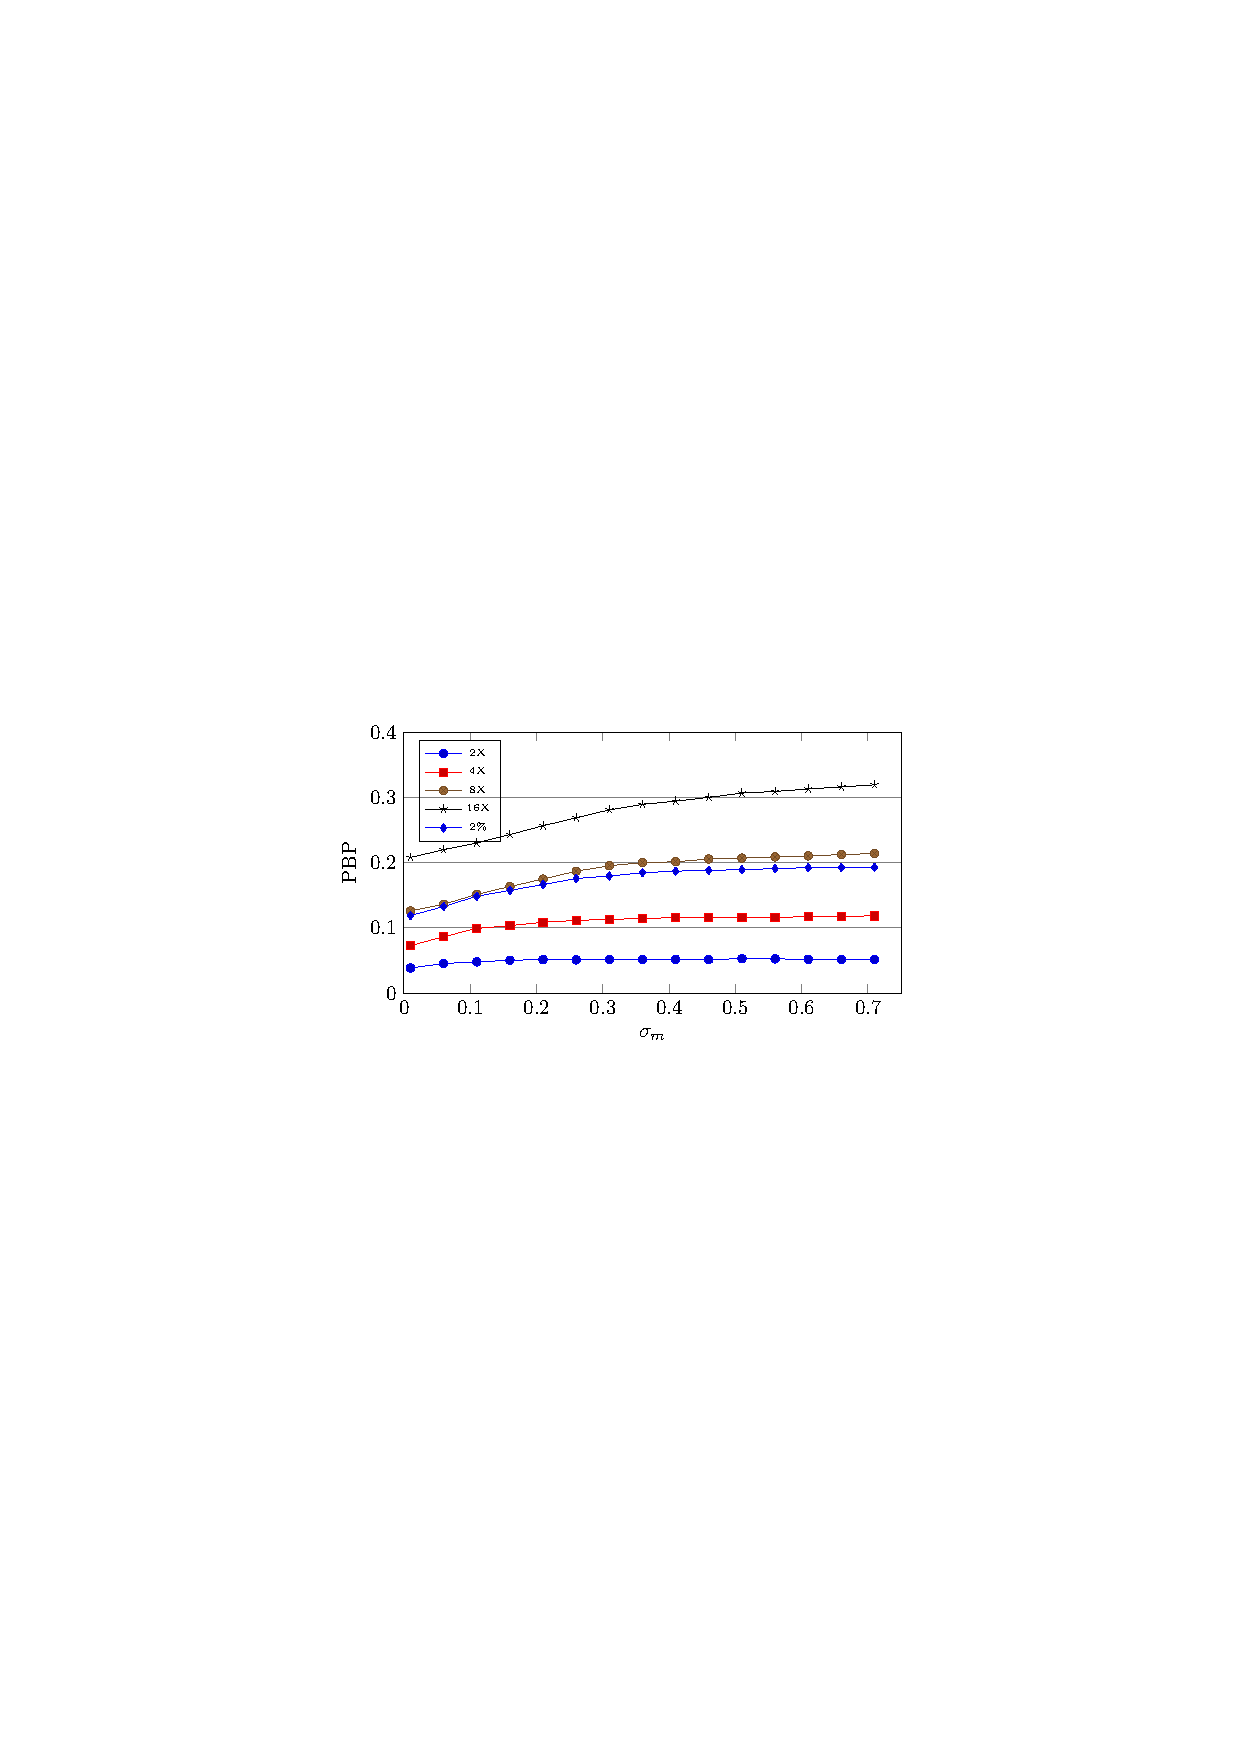
\includegraphics[width=\linewidth]{PBP1.pdf}
    %\captionsetup{skip=0pt}
    \caption{Discontinuous regions}
    \label{fig}
\end{subfigure}%
\begin{subfigure}[b]{0.35\linewidth}
    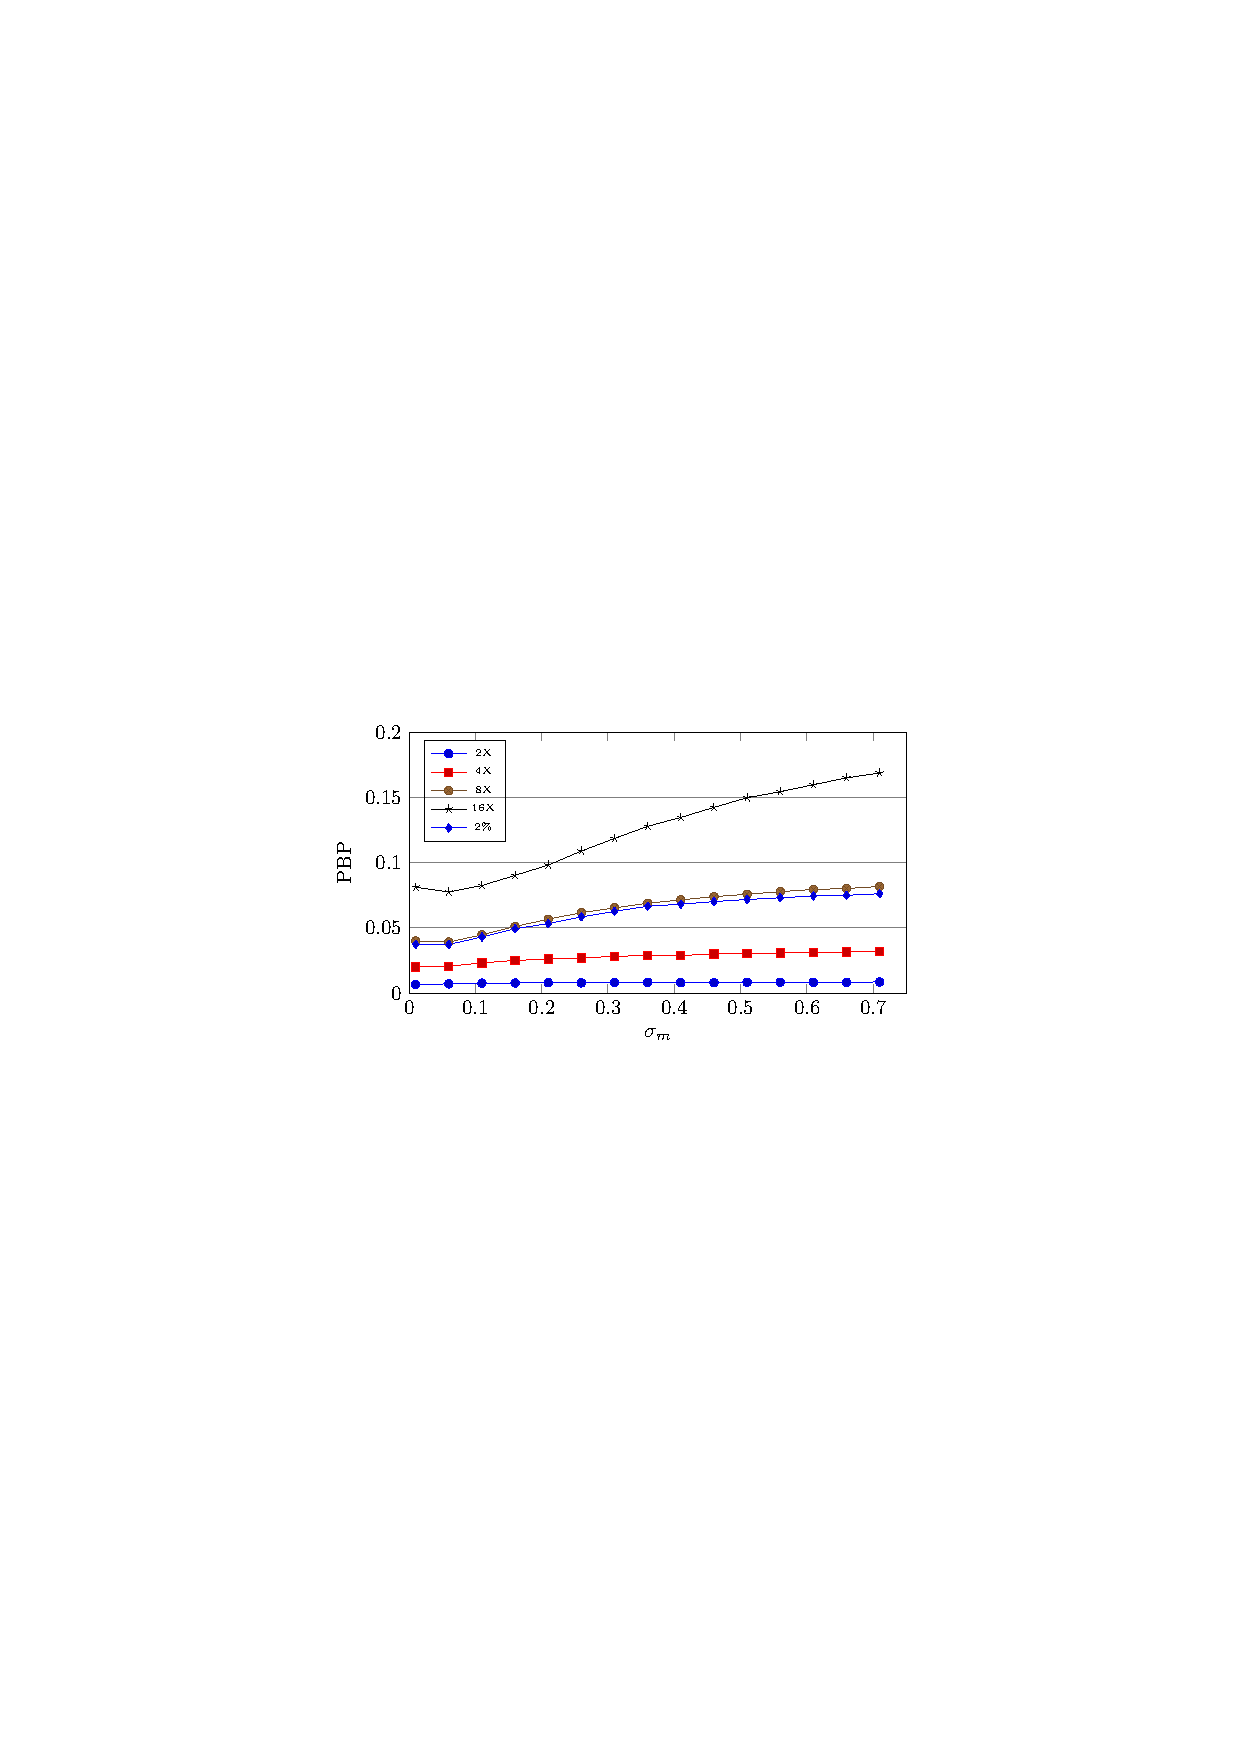
\includegraphics[width=\linewidth]{PBP2.pdf}
    %\captionsetup{skip=0pt}
    \caption{Continues areas}
    \label{fig:} %% label for first subfigure
 \end{subfigure}%
%\vspace{-0.3cm}
\caption{\textbf{Parameter sensitivity.} PBP performance curves of discontinuous regions and continuous areas are shown as a function of $\sigma_m$. The proposed algorithm renders good performance for a wide range of $\sigma_m$ under 2X, 4X, 8X, 16X upsampling rates and 2\% random missing inpainting.}
\label{fig:sensitivity}
%\vspace{-0.5cm}
\end{figure*}

In this section, only upsampling results are compared with seven methods~\cite{Liu2013,Yang2012,YangJingyu2012, Kopf2007,YangQingxiong2007,Choi_TIP_2014,Kang_ET_2014} on the Middlebury's benchmark~\cite{Hirschmuller2007} to verify the interpolation ability of our approach because these methods only focus on the depth upsampling and the interpolation quality of our method is independent of the seed distribution (refer to subsection~\ref{sec:sensitivity}). For fair comparison, we subscribe the 2X, 4X, 8X, 16X upsampling results of Art, Book, and Moebius from original authors. In the experiments, the low resolution depth images are obtained by downsampling and we use the percentage of bad matching pixels (PBP)~\cite{Scharstein2002} and the peak signal-to-noise ratio (PSNR)~\cite{Huynh_EL_2008} to evaluate the performance of discontinuous regions and continuous areas, where the discontinuous regions are obtained by dilating 1-pixel wide edge of ground truth and the rest of image domain $\Omega$ are considered as continuous areas. In literature, PBP estimates the interpolation quality via calculating the percentage of bad matching pixels and PSNR is an engineering term for the ratio between the maximum possible power of a signal and the power of corrupting noise that affects the fidelity of its representation.
The seven methods used for comparison are the joint bilateral upsampling (JBL)~\cite{Kopf2007}, the joint geodesic upsamping (JG)~\cite{Liu2013}, the bilateral filter upsampling with cost volume (BF)~\cite{YangQingxiong2007}, the non-local aggregation (NLA)~\cite{Yang2012}, the auto-regressive optimization (AR)~\cite{YangJingyu2012}, the structure and texture aware depth map upsampling (ST)~\cite{Choi_TIP_2014} and the depth local features upsampling (LF)~\cite{Kang_ET_2014}. In the following experiments, we assign $\sigma_m = 0.05$ consistently for our method because the parameter setting can produce satisfactory results for most situations according to our experience.


\begin{figure*}[t]
%\vspace{-0.5cm}
\begin{center}
%%%%%%%%%%%%%%%%%%%%%%%%%%%%%%%%%%%%%%%%%%%%%%%%%%%%%%%%%%%%%%%%%%
\vspace{-0.3cm}
\begin{subfigure}[b]{0.136\linewidth}
    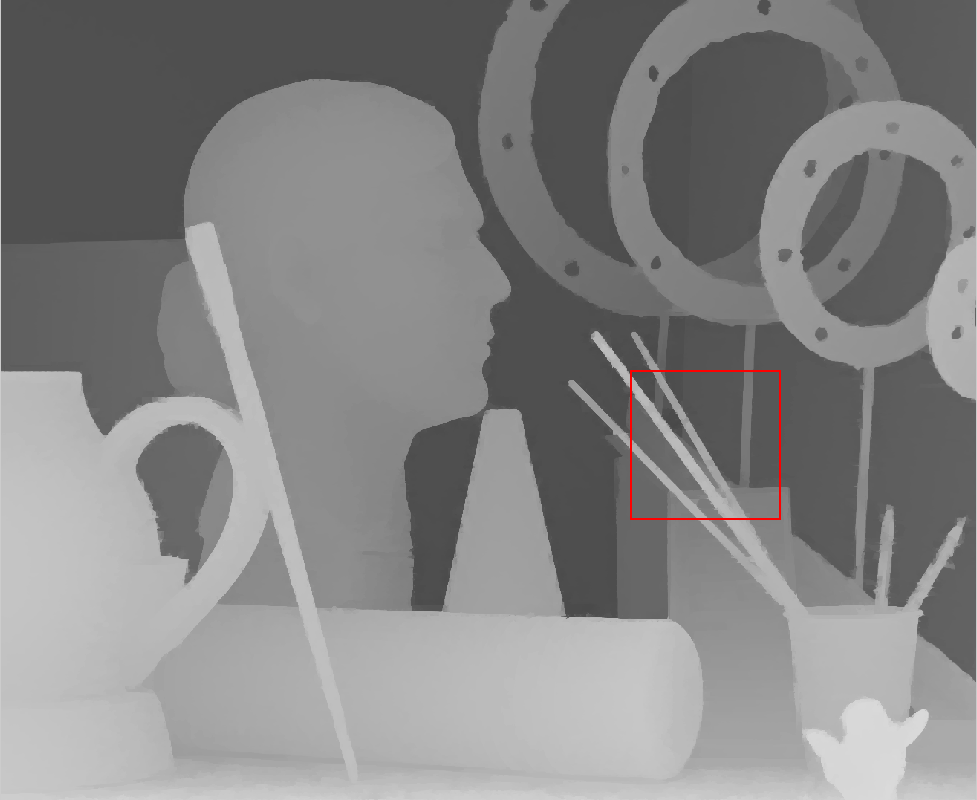
\includegraphics[width=\linewidth]{cmp_art_8X_JG.png}
    %\captionsetup{skip=5pt}
    \label{fig:}
\end{subfigure}
\begin{subfigure}[b]{0.136\linewidth}
    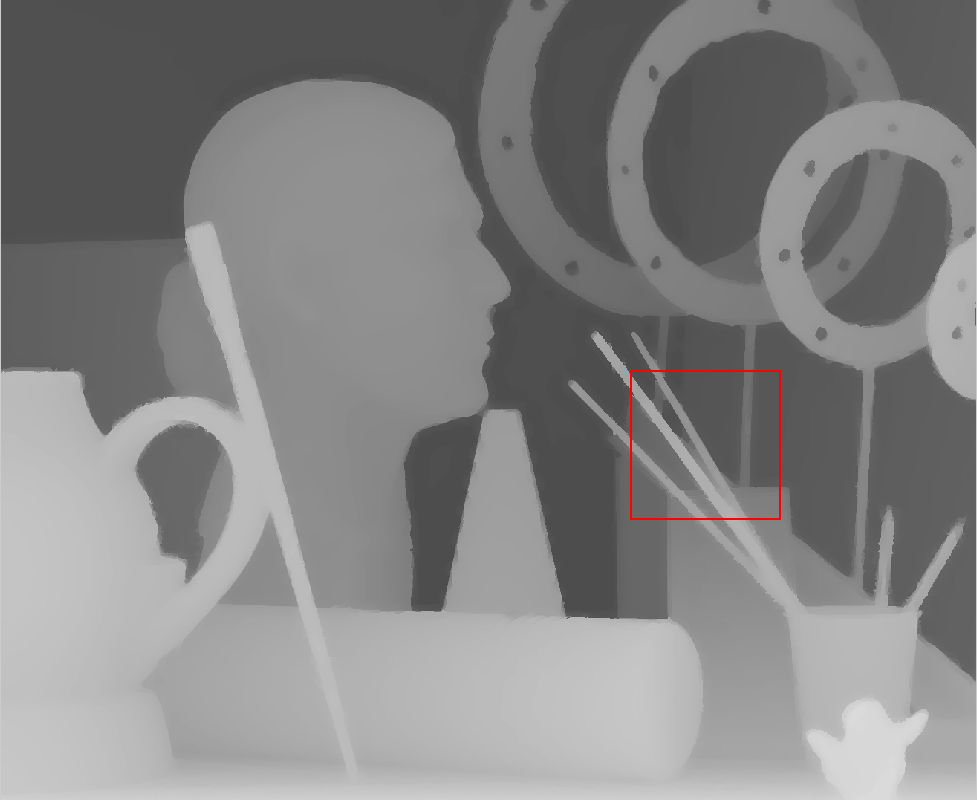
\includegraphics[width=\linewidth]{cmp_art_8X_NLA.png}
    \label{fig:} %% label for first subfigure
\end{subfigure}
\begin{subfigure}[b]{0.136\linewidth}
    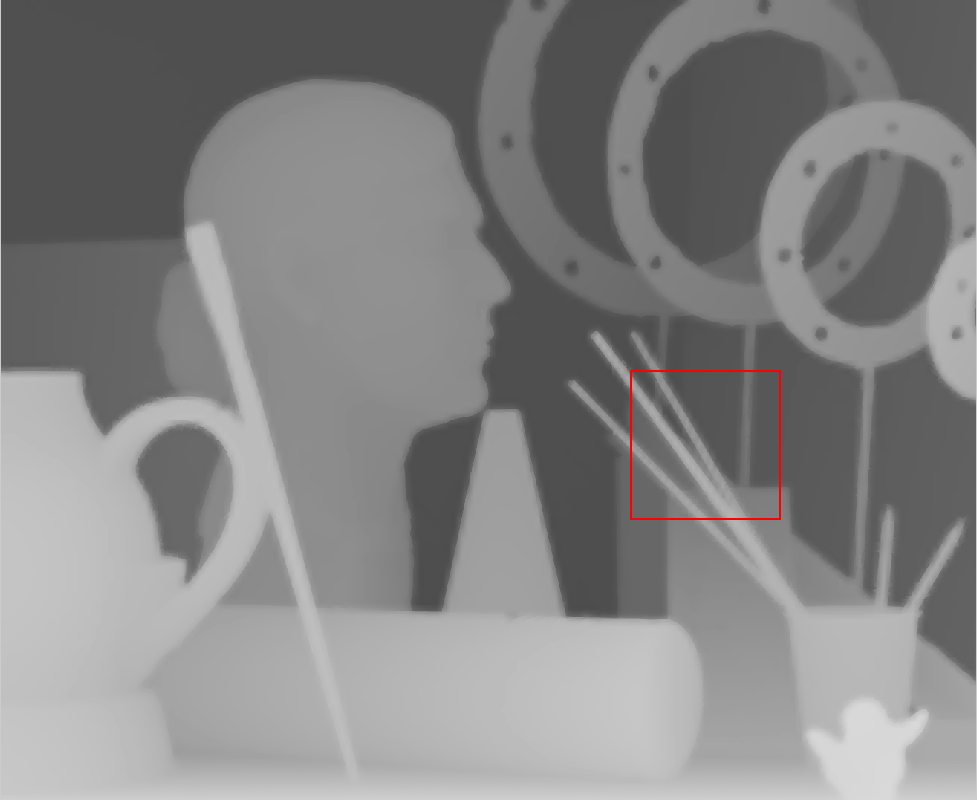
\includegraphics[width=\linewidth]{cmp_art_8X_JBL.png}
    %\captionsetup{skip=5pt}
    \label{fig:}
\end{subfigure}
\begin{subfigure}[b]{0.136\linewidth}
    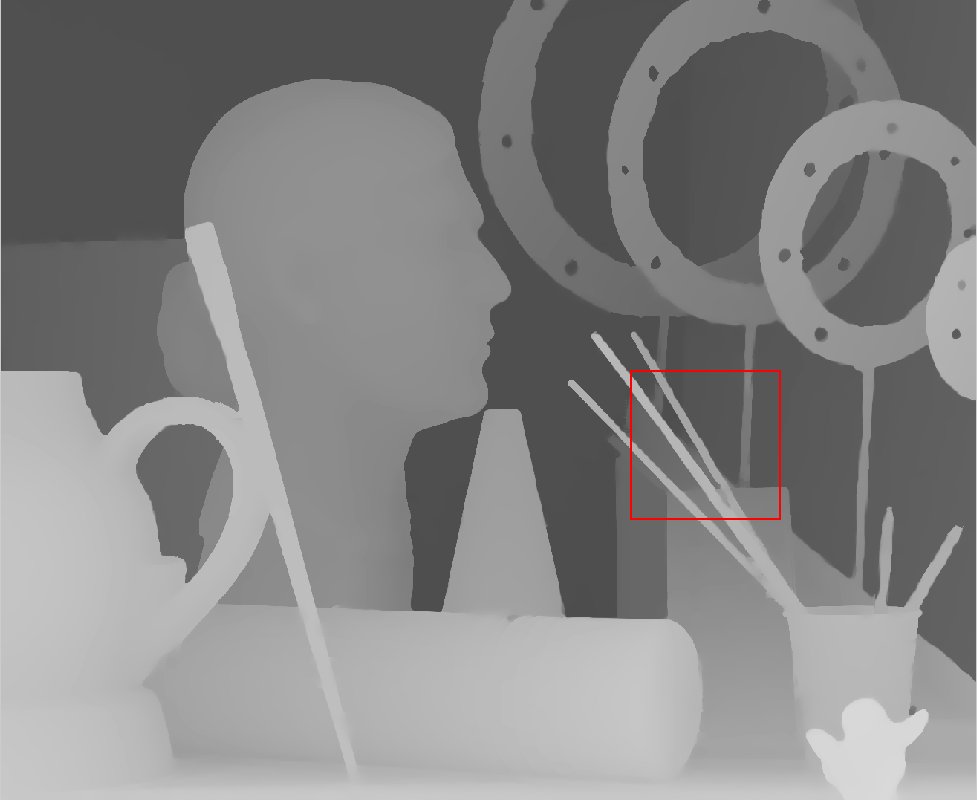
\includegraphics[width=\linewidth]{cmp_art_8X_AR.png}
    \label{fig:} %% label for first subfigure
\end{subfigure}
\begin{subfigure}[b]{0.136\linewidth}
    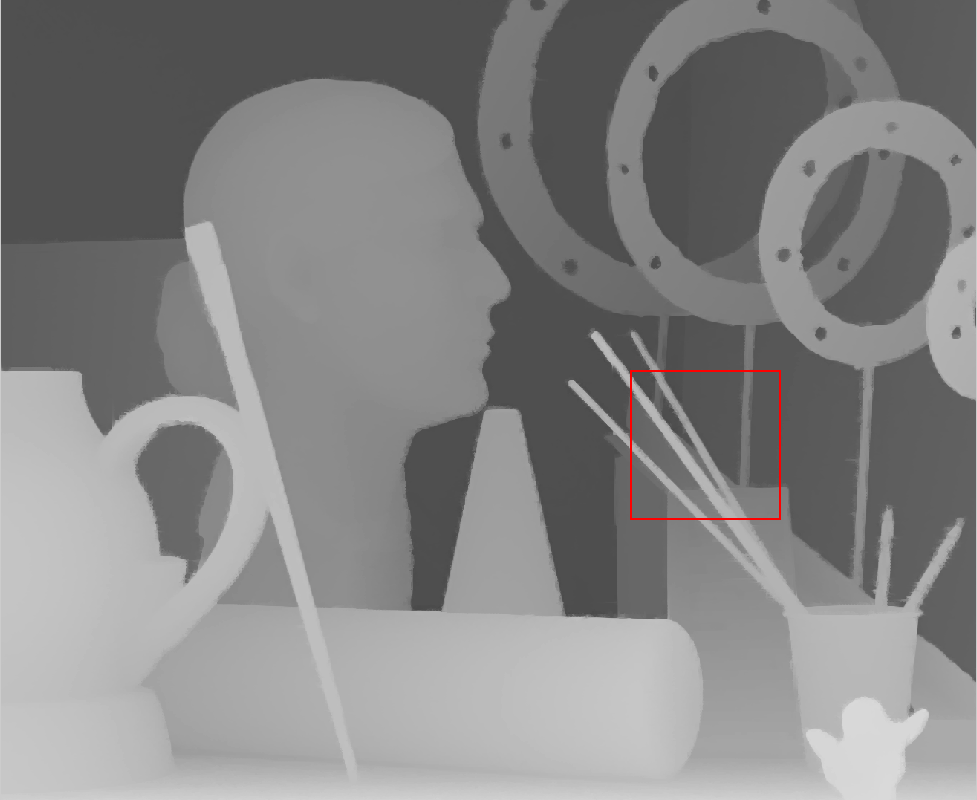
\includegraphics[width=\linewidth]{cmp_art_8X_ST.png}
    %\captionsetup{skip=5pt}
    \label{fig:}
\end{subfigure}
\begin{subfigure}[b]{0.136\linewidth}
    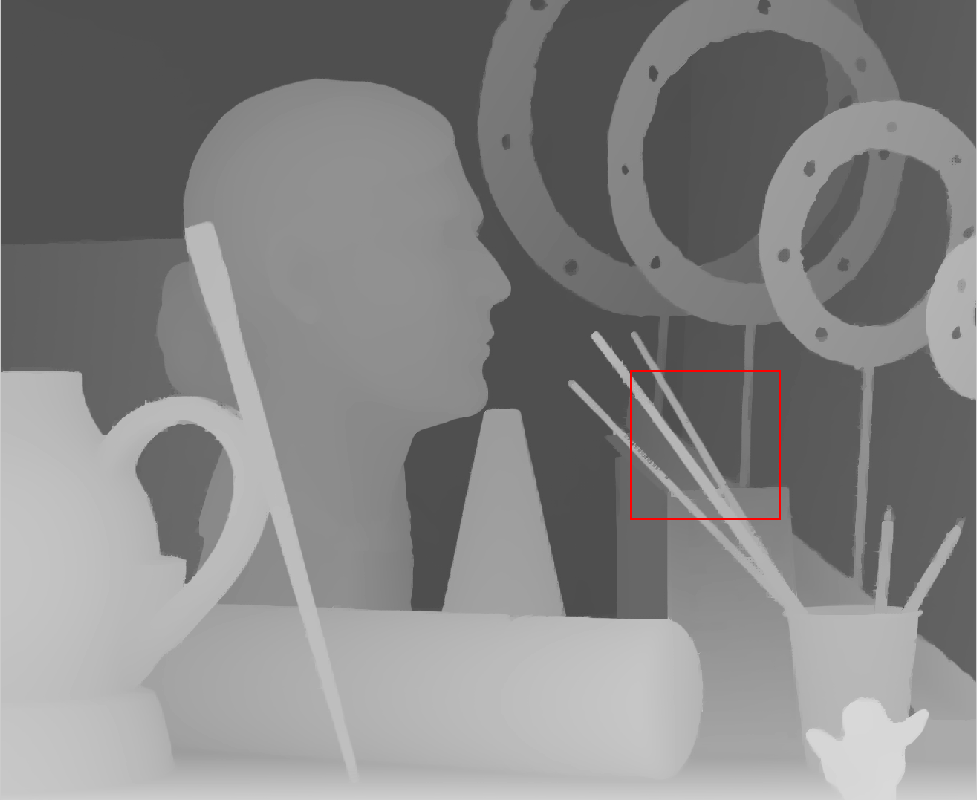
\includegraphics[width=\linewidth]{cmp_art_8X_LF.png}
    \label{fig:} %% label for first subfigure
\end{subfigure}
\begin{subfigure}[b]{0.136\linewidth}
    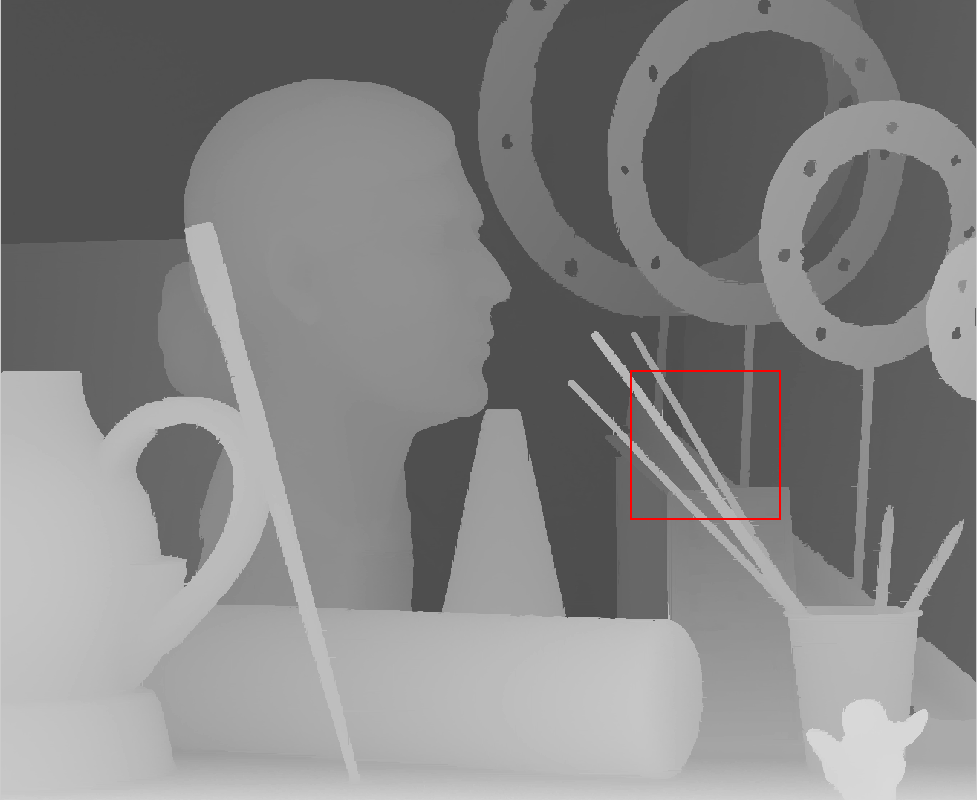
\includegraphics[width=\linewidth]{cmp_art_8X_MST.png}
    \label{fig:} %% label for first subfigure
\end{subfigure}

%%%%%%%%%%%%%%%%%%%%%%%%%%%%%%%%%%%%%%%%%%%%%%%%%%%%%%%%%%%%%%%%%%
\vspace{-0.3cm}
\begin{subfigure}[b]{0.136\linewidth}
    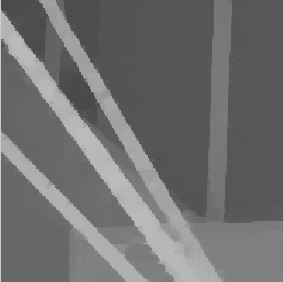
\includegraphics[height = 2cm,width=\linewidth]{cmp_art_8X_JG_part.png}
    %\captionsetup{skip=5pt}
    \label{fig:}
\end{subfigure}
\begin{subfigure}[b]{0.136\linewidth}
    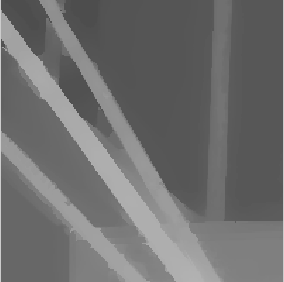
\includegraphics[height = 2cm,width=\linewidth]{cmp_art_8X_NLA_part.png}
    \label{fig:} %% label for first subfigure
\end{subfigure}
\begin{subfigure}[b]{0.136\linewidth}
    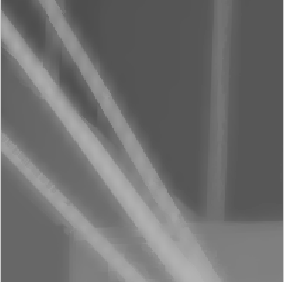
\includegraphics[height = 2cm,width=\linewidth]{cmp_art_8X_JBL_part.png}
    %\captionsetup{skip=5pt}
    \label{fig:}
\end{subfigure}
\begin{subfigure}[b]{0.136\linewidth}
    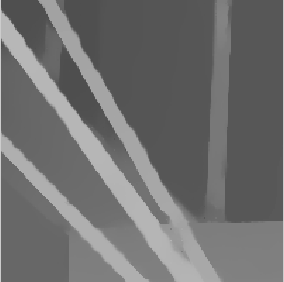
\includegraphics[height = 2cm,width=\linewidth]{cmp_art_8X_AR_part.png}
    \label{fig:} %% label for first subfigure
\end{subfigure}
\begin{subfigure}[b]{0.136\linewidth}
    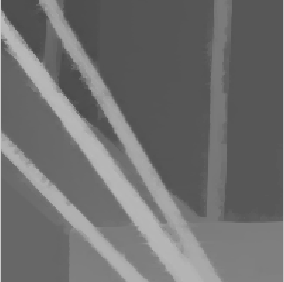
\includegraphics[height = 2cm,width=\linewidth]{cmp_art_8X_ST_part.png}
    %\captionsetup{skip=5pt}
    \label{fig:}
\end{subfigure}
\begin{subfigure}[b]{0.136\linewidth}
    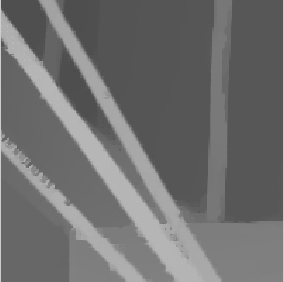
\includegraphics[height = 2cm,width=\linewidth]{cmp_art_8X_LF_part.png}
    \label{fig:} %% label for first subfigure
\end{subfigure}
\begin{subfigure}[b]{0.136\linewidth}
    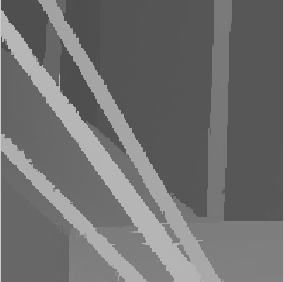
\includegraphics[height = 2cm,width=\linewidth]{cmp_art_8X_MST_part.png}
    \label{fig:} %% label for first subfigure
\end{subfigure}

%%%%%%%%%%%%%%%%%%%%%%%%%%%%%%%%%%%%%%%%%%%%%%%%%%%%%%%%%%%%%%%%%%
\vspace{-0.3cm}
\begin{subfigure}[b]{0.136\linewidth}
    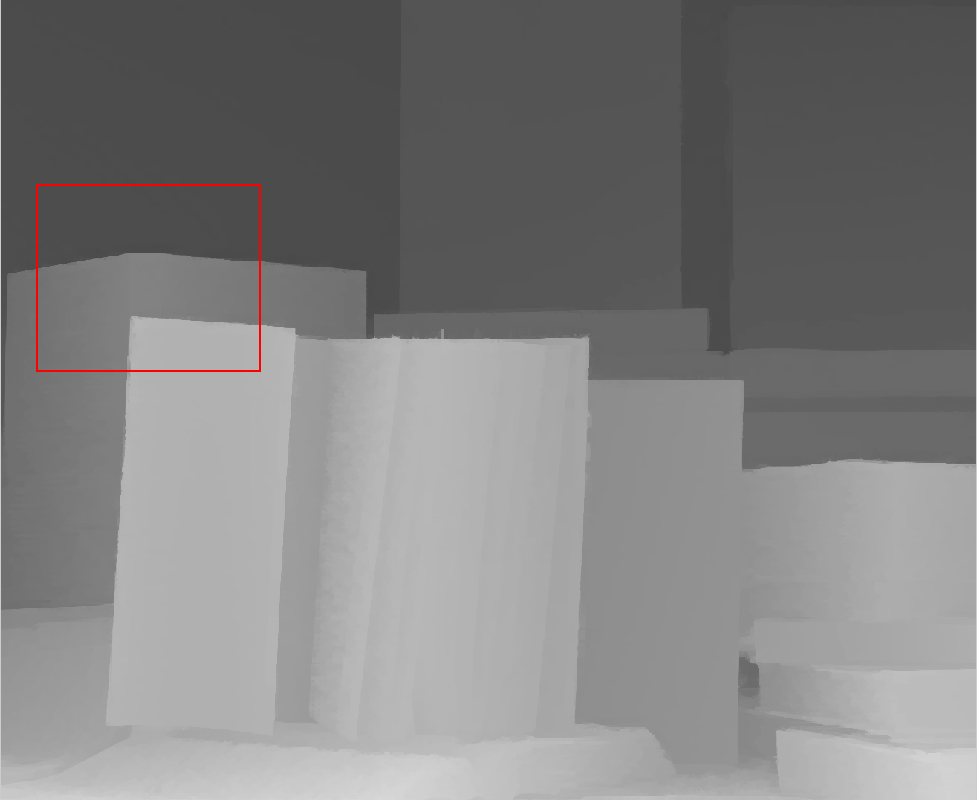
\includegraphics[width=\linewidth]{cmp_book_8X_JG.png}
    %\captionsetup{skip=5pt}
    \label{fig:}
\end{subfigure}
\begin{subfigure}[b]{0.136\linewidth}
    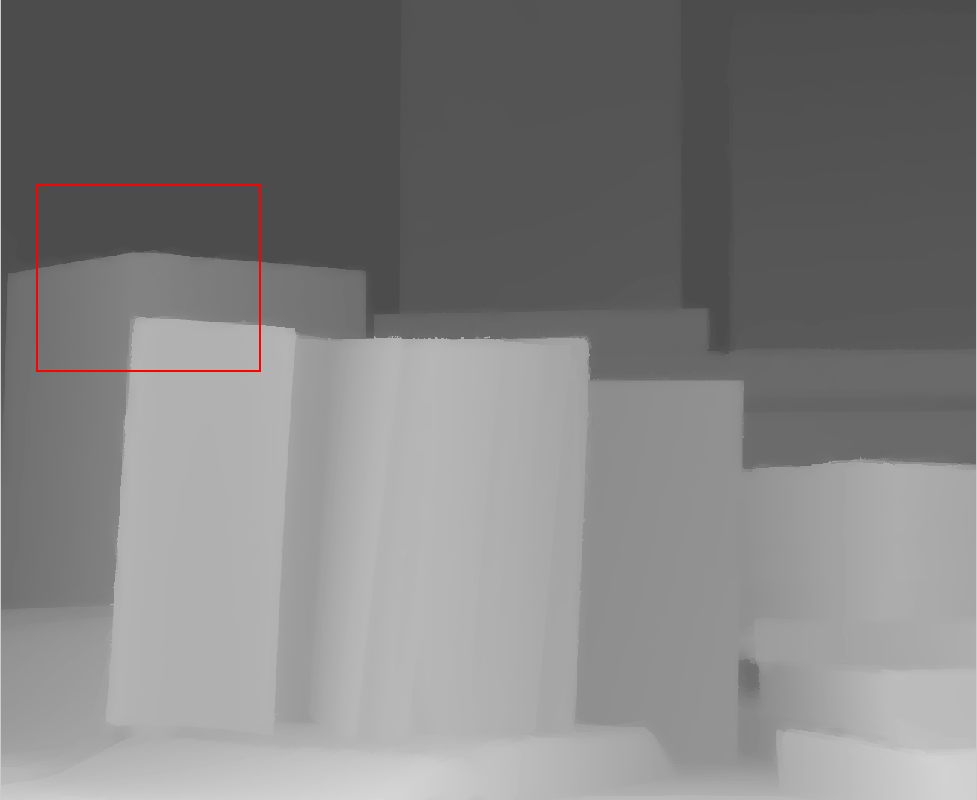
\includegraphics[width=\linewidth]{cmp_book_8X_NLA.png}
    \label{fig:} %% label for first subfigure
\end{subfigure}
\begin{subfigure}[b]{0.136\linewidth}
    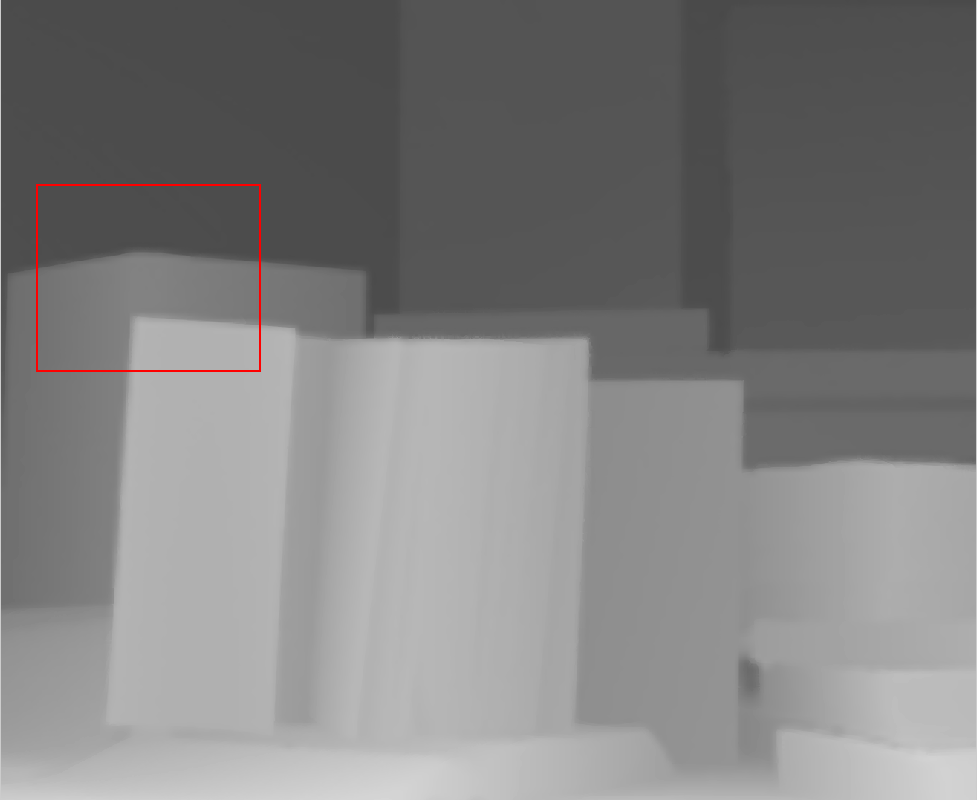
\includegraphics[width=\linewidth]{cmp_book_8X_JBL.png}
    %\captionsetup{skip=5pt}
    \label{fig:}
\end{subfigure}
\begin{subfigure}[b]{0.136\linewidth}
    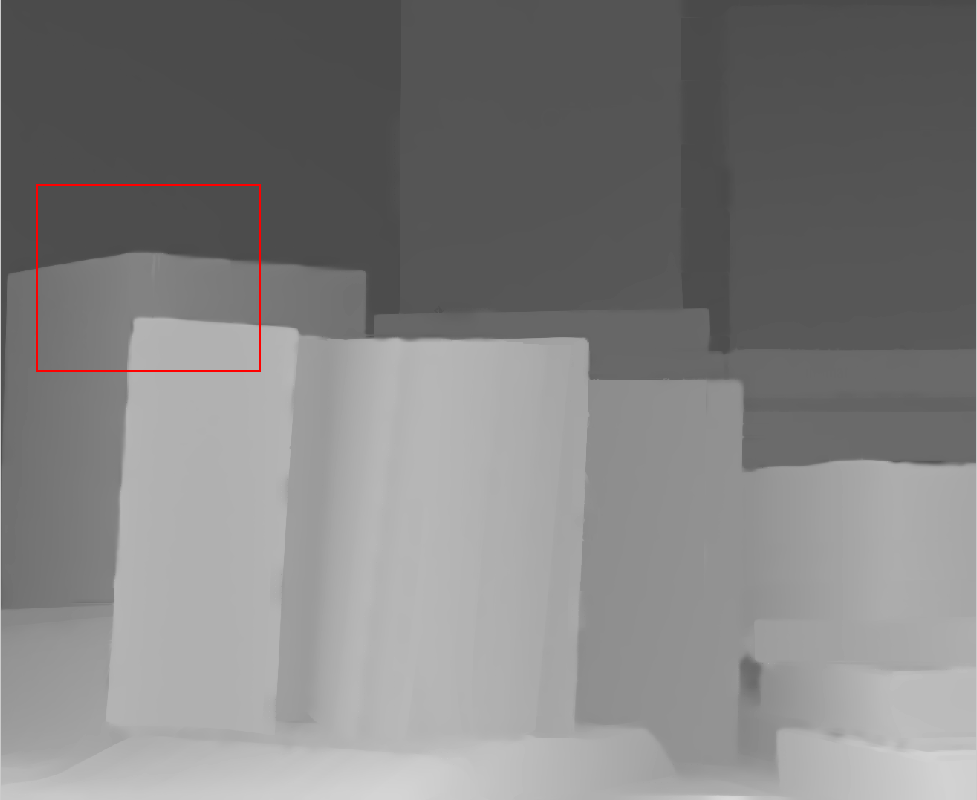
\includegraphics[width=\linewidth]{cmp_book_8X_AR.png}
    \label{fig:} %% label for first subfigure
\end{subfigure}
\begin{subfigure}[b]{0.136\linewidth}
    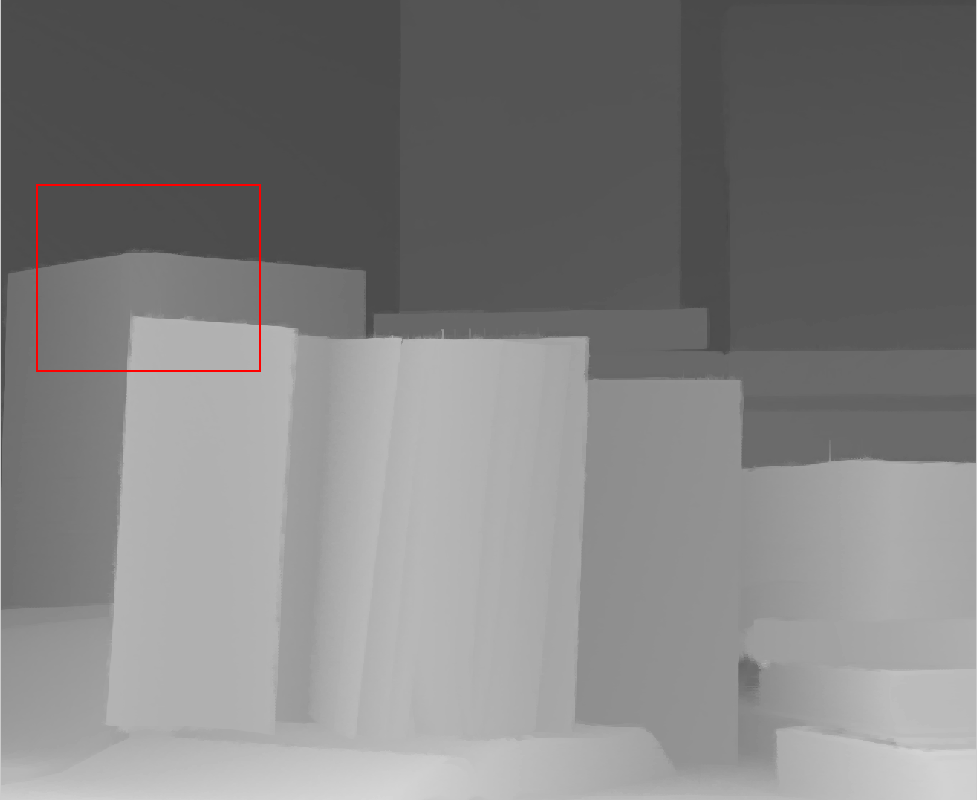
\includegraphics[width=\linewidth]{cmp_book_8X_ST.png}
    %\captionsetup{skip=5pt}
    \label{fig:}
\end{subfigure}
\begin{subfigure}[b]{0.136\linewidth}
    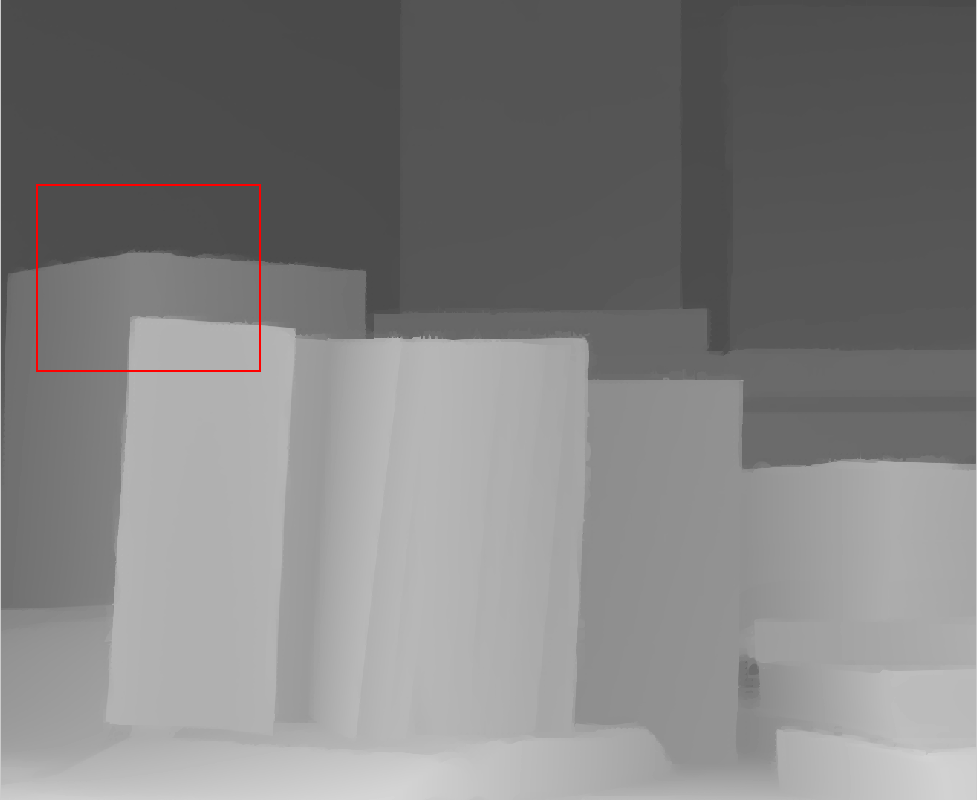
\includegraphics[width=\linewidth]{cmp_book_8X_LF.png}
    \label{fig:} %% label for first subfigure
\end{subfigure}
\begin{subfigure}[b]{0.136\linewidth}
    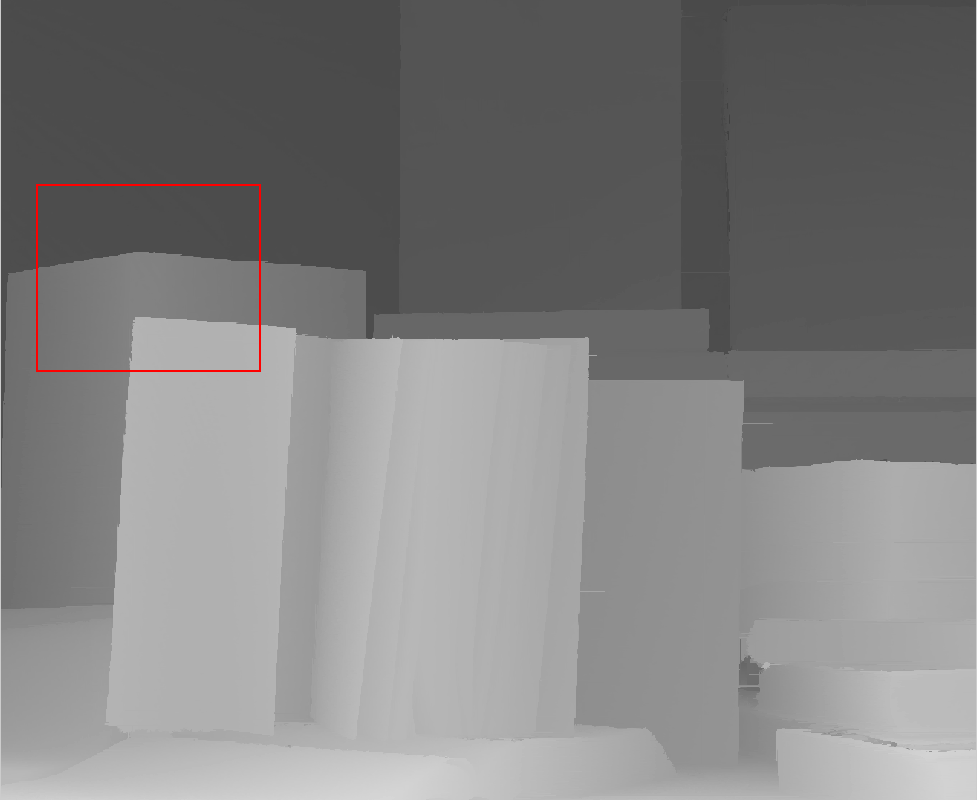
\includegraphics[width=\linewidth]{cmp_book_8X_MST.png}
    \label{fig:} %% label for first subfigure
\end{subfigure}

%%%%%%%%%%%%%%%%%%%%%%%%%%%%%%%%%%%%%%%%%%%%%%%%%%%%%%%%%%%%%%%%%%
\vspace{-0.3cm}
\begin{subfigure}[b]{0.136\linewidth}
    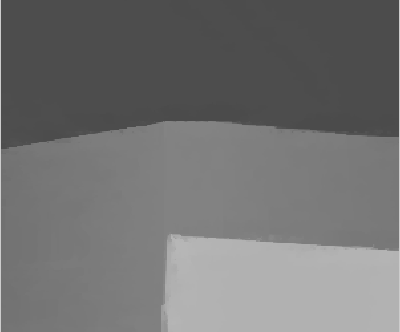
\includegraphics[width=\linewidth]{cmp_book_8X_JG_part.png}
    %\captionsetup{skip=5pt}
    \label{fig:}
\end{subfigure}
\begin{subfigure}[b]{0.136\linewidth}
    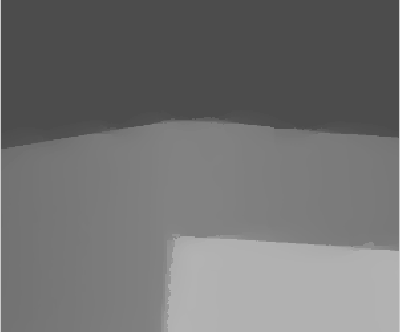
\includegraphics[width=\linewidth]{cmp_book_8X_NLA_part.png}
    \label{fig:} %% label for first subfigure
\end{subfigure}
\begin{subfigure}[b]{0.136\linewidth}
    
\includegraphics[width=\linewidth]{cmp_book_8X_JBL_part.png}
    %\captionsetup{skip=5pt}
    \label{fig:}
\end{subfigure}
\begin{subfigure}[b]{0.136\linewidth}
    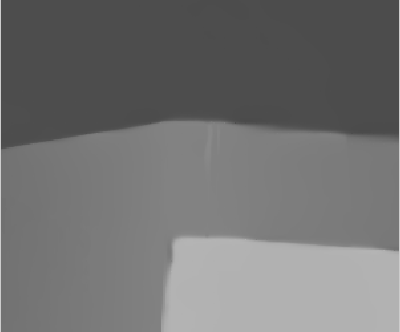
\includegraphics[width=\linewidth]{cmp_book_8X_AR_part.png}
    \label{fig:} %% label for first subfigure
\end{subfigure}
\begin{subfigure}[b]{0.136\linewidth}
    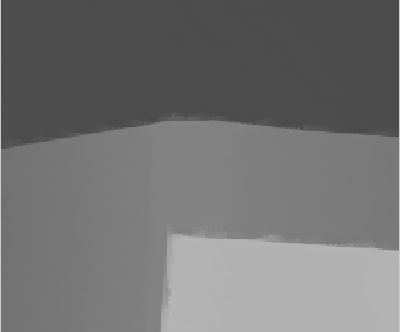
\includegraphics[width=\linewidth]{cmp_book_8X_ST_part.png}
    %\captionsetup{skip=5pt}
    \label{fig:}
\end{subfigure}
\begin{subfigure}[b]{0.136\linewidth}
    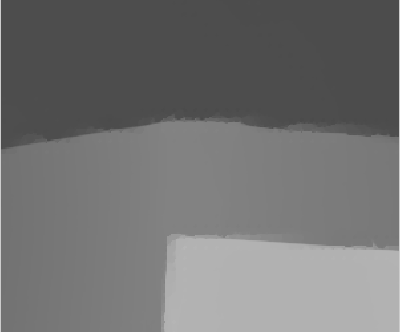
\includegraphics[width=\linewidth]{cmp_book_8X_LF_part.png}
    \label{fig:} %% label for first subfigure
\end{subfigure}
\begin{subfigure}[b]{0.136\linewidth}
    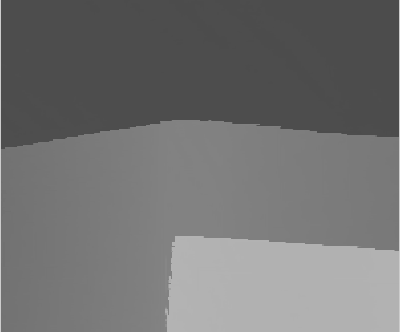
\includegraphics[width=\linewidth]{cmp_book_8X_MST_part.png}
    \label{fig:} %% label for first subfigure
\end{subfigure}

%%%%%%%%%%%%%%%%%%%%%%%%%%%%%%%%%%%%%%%%%%%%%%%%%%%%%%%%%%%%%%%%%%
\vspace{-0.3cm}
\begin{subfigure}[b]{0.136\linewidth}
    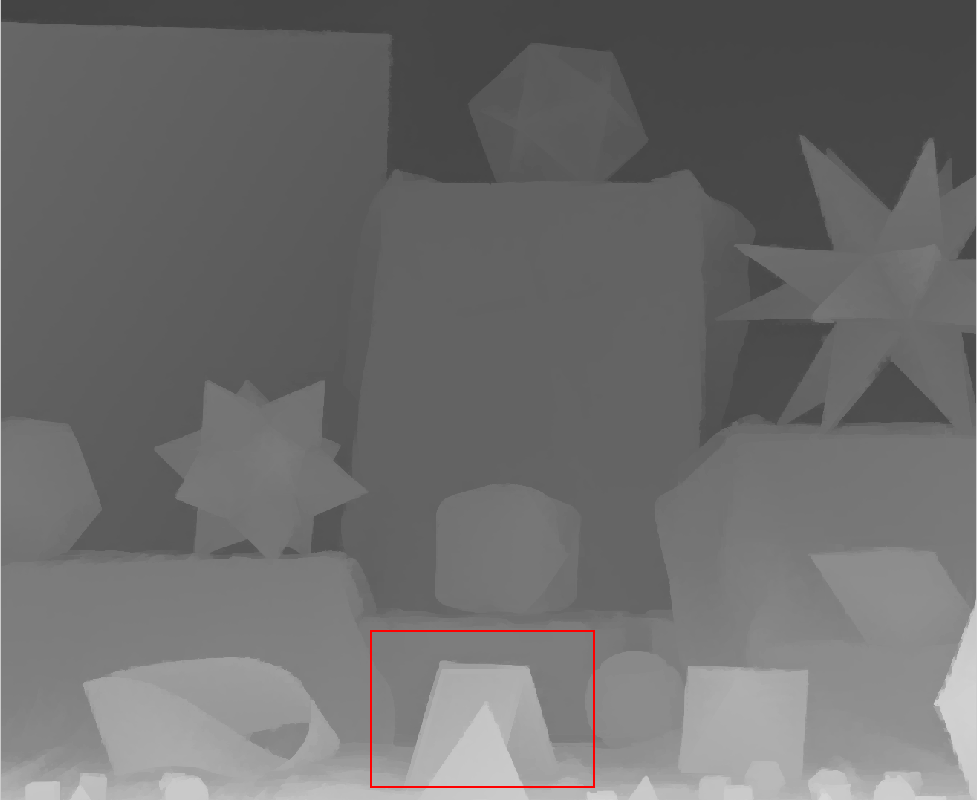
\includegraphics[width=\linewidth]{cmp_moebius_8X_JG.png}
    %\captionsetup{skip=5pt}
    \label{fig:}
\end{subfigure}
\begin{subfigure}[b]{0.136\linewidth}
    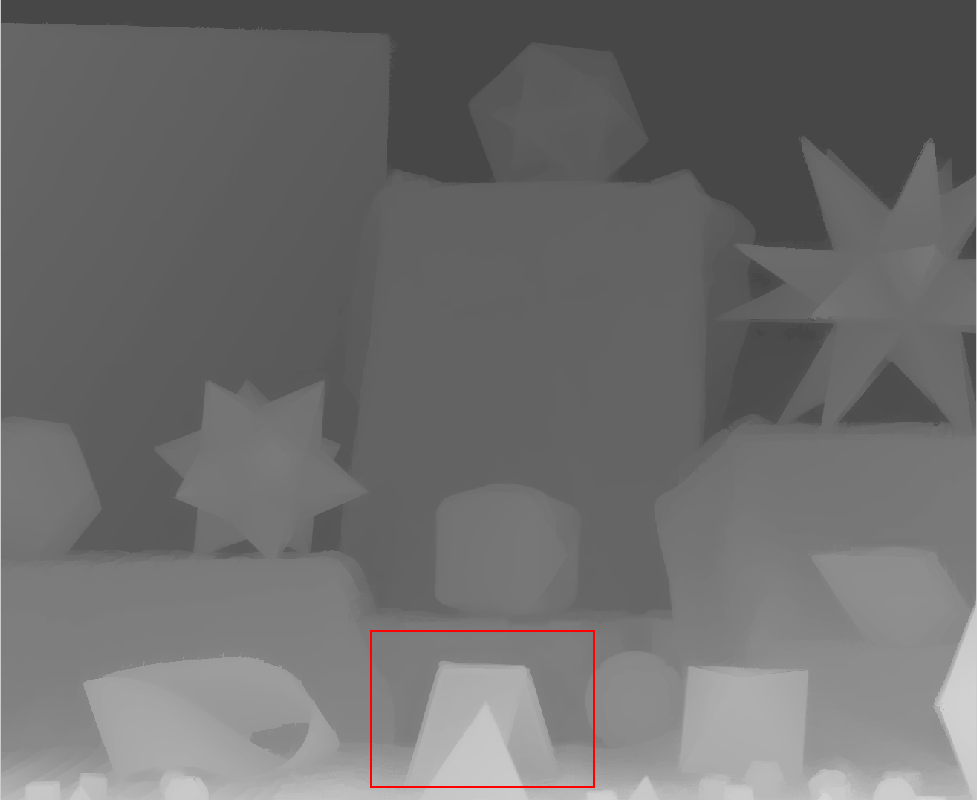
\includegraphics[width=\linewidth]{cmp_moebius_8X_NLA.png}
    \label{fig:} %% label for first subfigure
\end{subfigure}
\begin{subfigure}[b]{0.136\linewidth}
    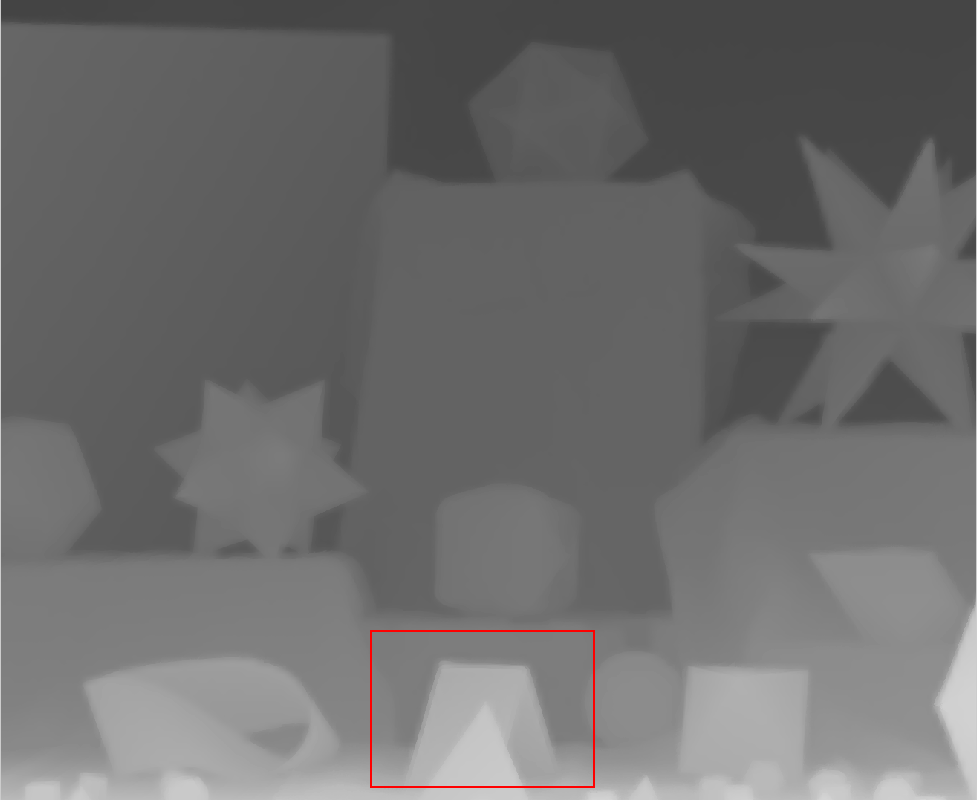
\includegraphics[width=\linewidth]{cmp_moebius_8X_JBL.png}
    %\captionsetup{skip=5pt}
    \label{fig:}
\end{subfigure}
\begin{subfigure}[b]{0.136\linewidth}
    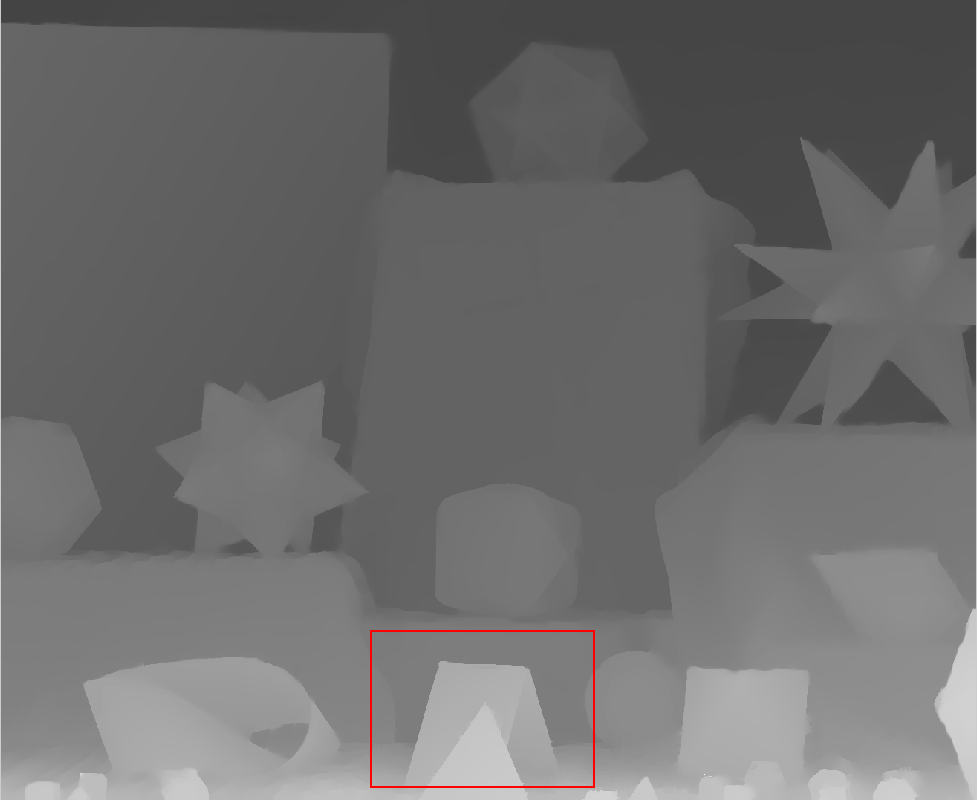
\includegraphics[width=\linewidth]{cmp_moebius_8X_AR.png}
    \label{fig:} %% label for first subfigure
\end{subfigure}
\begin{subfigure}[b]{0.136\linewidth}
    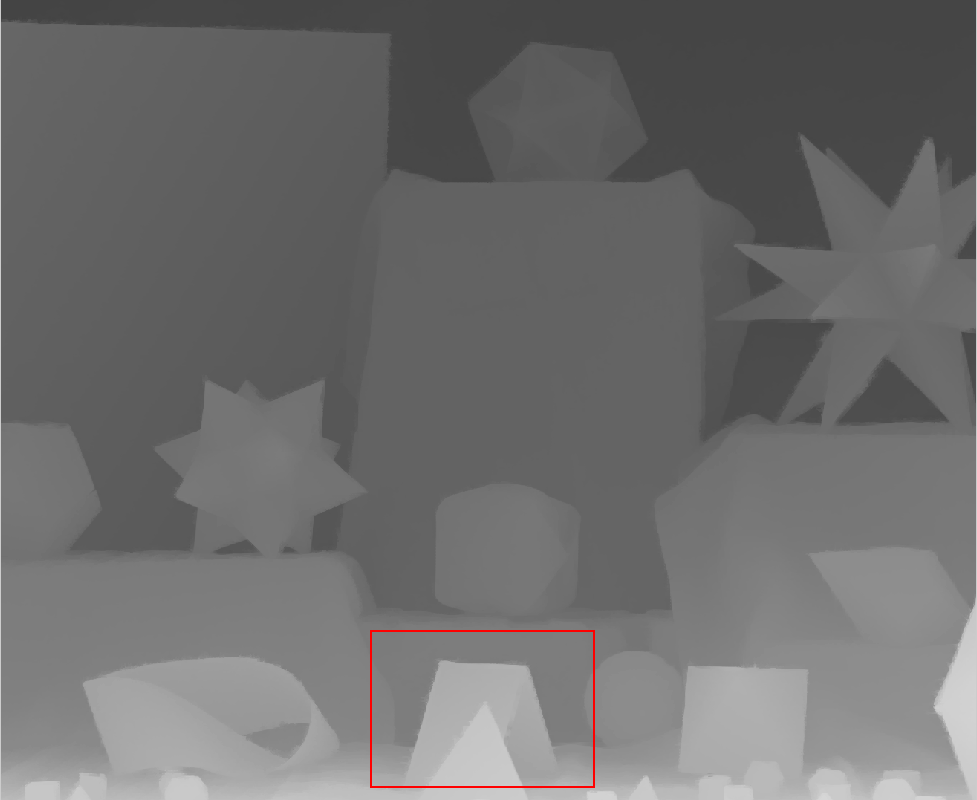
\includegraphics[width=\linewidth]{cmp_moebius_8X_ST.png}
    %\captionsetup{skip=5pt}
    \label{fig:}
\end{subfigure}
\begin{subfigure}[b]{0.136\linewidth}
    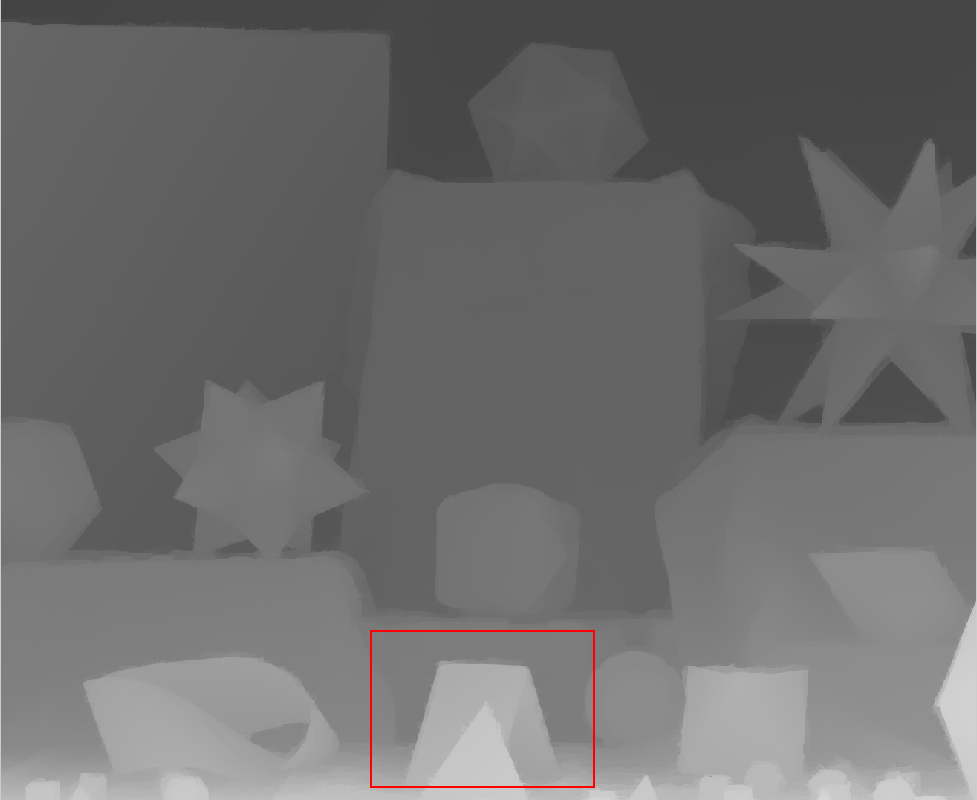
\includegraphics[width=\linewidth]{cmp_moebius_8X_LF.png}
    \label{fig:} %% label for first subfigure
\end{subfigure}
\begin{subfigure}[b]{0.136\linewidth}
    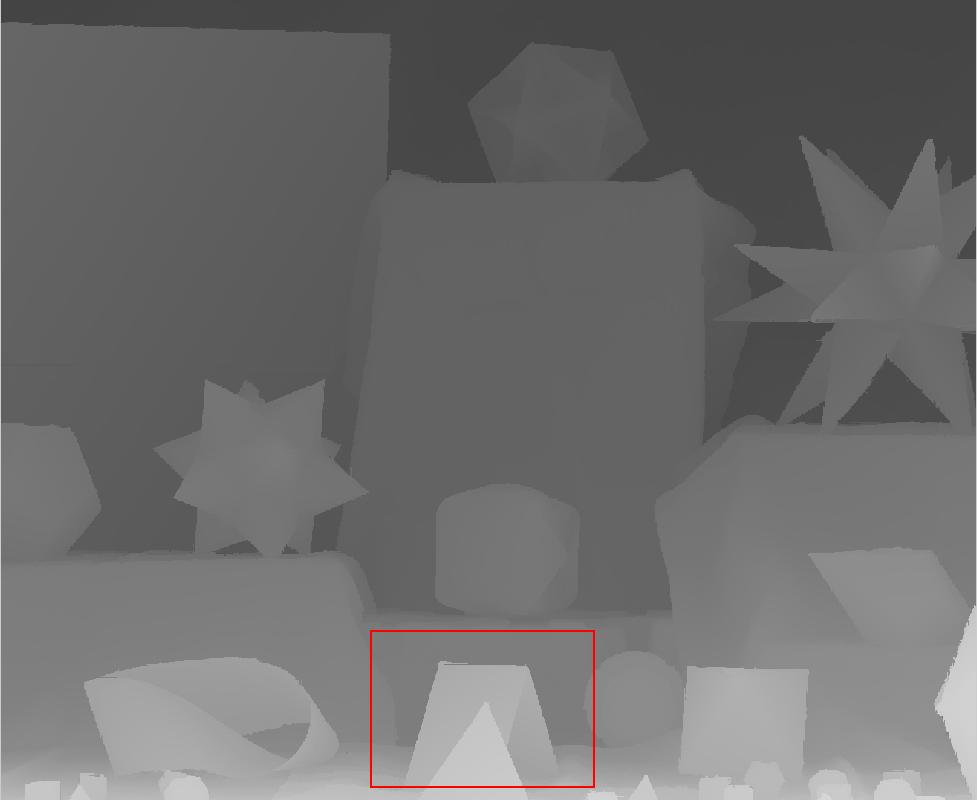
\includegraphics[width=\linewidth]{cmp_moebius_8X_MST.png}
    \label{fig:} %% label for first subfigure
\end{subfigure}

%%%%%%%%%%%%%%%%%%%%%%%%%%%%%%%%%%%%%%%%%%%%%%%%%%%%%%%%%%%%%%%%%%
\vspace{-0.3cm}
\begin{subfigure}[b]{0.136\linewidth}
    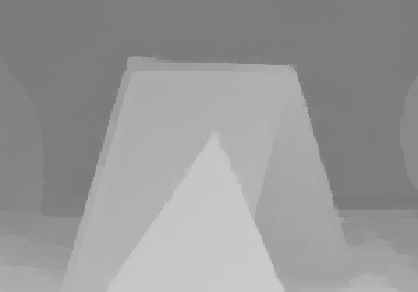
\includegraphics[height = 2cm,width=\linewidth]{cmp_moebius_8X_JG_part.png}
    \caption{AR~\cite{YangJingyu2012}}
    %\captionsetup{skip=5pt}
    \label{fig:AR}
\end{subfigure}
\begin{subfigure}[b]{0.136\linewidth}
    
\includegraphics[height = 2cm,width=\linewidth]{cmp_moebius_8X_NLA_part.png}
    \caption{NLA~\cite{Yang2012}}
    \label{fig:NLA} %% label for first subfigure
\end{subfigure}
\begin{subfigure}[b]{0.136\linewidth}
    
\includegraphics[height = 2cm,width=\linewidth]{cmp_moebius_8X_JBL_part.png}
    %\captionsetup{skip=5pt}
    \caption{JBL~\cite{Kopf2007}}
    \label{fig:JBL}
\end{subfigure}
\begin{subfigure}[b]{0.136\linewidth}
    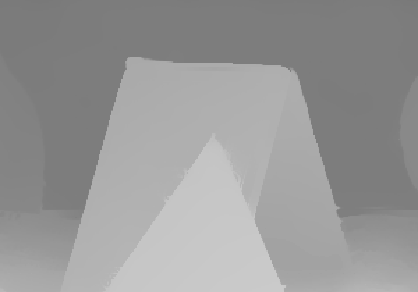
\includegraphics[height = 2cm,width=\linewidth]{cmp_moebius_8X_AR_part.png}
    \caption{JG~\cite{Liu2013}}
    \label{fig:JG} %% label for first subfigure
\end{subfigure}
\begin{subfigure}[b]{0.136\linewidth}
    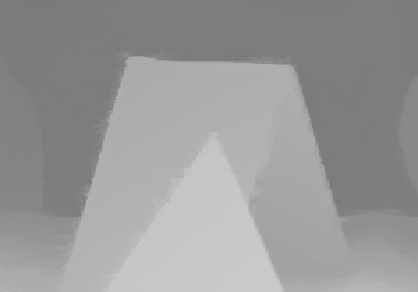
\includegraphics[height = 2cm,width=\linewidth]{cmp_moebius_8X_ST_part.png}
    %\captionsetup{skip=5pt}
    \caption{ST~\cite{Choi_TIP_2014}}
    \label{fig:ST}
\end{subfigure}
\begin{subfigure}[b]{0.136\linewidth}
    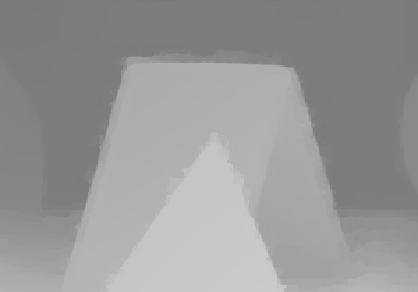
\includegraphics[height = 2cm,width=\linewidth]{cmp_moebius_8X_LF_part.png}
    \caption{LF~\cite{Kang_ET_2014}}
    \label{fig:LF} %% label for first subfigure
\end{subfigure}
\begin{subfigure}[b]{0.136\linewidth}
    \includegraphics[height = 2cm,width=\linewidth]{cmp_moebius_8X_MST_part.png}
    \caption{Ours}
    \label{fig:ours} %% label for first subfigure
\end{subfigure}
\end{center}
%\vspace{-0.6cm}
\caption{\textbf{Visual comparison.} Visual comparison of the upsampling results at 8X upsampling rate. From left to right, each column corresponds to the results of AR~\cite{YangJingyu2012}, NLA~\cite{Yang2012}, JBL~\cite{Kopf2007}, JG~\cite{Liu2013}, ST~\cite{Choi_TIP_2014}, LF~\cite{Kang_ET_2014} and ours, respectively. Our method produces the best upsampling results with sharpest edges and fewest artifacts. }
\label{fig:comparison}
%\vspace{-0.5cm}
\end{figure*}


\begin{figure*}[t]
%\vspace{-0.5cm}
\begin{center}
\begin{subfigure}[b]{0.136\linewidth}
    \includegraphics[width=\linewidth]{desk_structure_missing_color.png}
\end{subfigure}
\begin{subfigure}[b]{0.136\linewidth}
    \includegraphics[width=\linewidth]{desk_structure_missing_depth.png}
\end{subfigure}
\begin{subfigure}[b]{0.136\linewidth}
    \includegraphics[width=\linewidth]{desk_structure_missing_inpainting.png}
\end{subfigure}
\begin{subfigure}[b]{0.136\linewidth}
    \includegraphics[width=\linewidth]{desk_random_missing_depth.png}
\end{subfigure}
\begin{subfigure}[b]{0.136\linewidth}
    \includegraphics[width=\linewidth]{desk_random_missing_inpainting.png}
\end{subfigure}
\begin{subfigure}[b]{0.136\linewidth}
    \includegraphics[width=\linewidth]{desk_upsampling_depth.png}
\end{subfigure}
\begin{subfigure}[b]{0.136\linewidth}
    \includegraphics[width=\linewidth]{desk_upsampling_inpainting.png}
\end{subfigure}

%%%%%%%%%%%%%%%%%%%%%%%%%%%%%%%%%%%%%%%%%%%%%%%%%%%%%%%%%%%%%%%%%%
%\vspace{-0.4cm}
\begin{subfigure}[b]{0.136\linewidth}
    \includegraphics[width=\linewidth]{table_structure_missing_color.png}
    %\captionsetup{skip=2pt}
\end{subfigure}
\begin{subfigure}[b]{0.136\linewidth}
    \includegraphics[width=\linewidth]{table_structure_missing_depth.png}
    %\captionsetup{skip=2pt}
\end{subfigure}
\begin{subfigure}[b]{0.136\linewidth}
    \includegraphics[width=\linewidth]{table_structure_missing_inpainting.png}
    %\captionsetup{skip=2pt}
\end{subfigure}
\begin{subfigure}[b]{0.136\linewidth}
    \includegraphics[width=\linewidth]{table_random_missing_depth.png}
    %\captionsetup{skip=2pt}
\end{subfigure}
\begin{subfigure}[b]{0.136\linewidth}
    \includegraphics[width=\linewidth]{table_random_missing_inpainting.png}
    %\captionsetup{skip=2pt}
\end{subfigure}
\begin{subfigure}[b]{0.136\linewidth}
    \includegraphics[width=\linewidth]{table_upsampling_depth.png}
    %\includegraphics[width=\linewidth]{t.png}
    %\captionsetup{skip=2pt}
\end{subfigure}
\begin{subfigure}[b]{0.136\linewidth}
    \includegraphics[width=\linewidth]{table_upsampling_inpainting.png}
    %\captionsetup{skip=2pt}
\end{subfigure}

%%%%%%%%%%%%%%%%%%%%%%%%%%%%%%%%%%%%%%%%%%%%%%%%%%%%%%%%%%%%%%%%%%
%\vspace{-0.4cm}
\begin{subfigure}[b]{0.136\linewidth}
    \includegraphics[width=\linewidth]{sofa_structure_missing_color.png}
    %\captionsetup{skip=2pt}
\end{subfigure}
\begin{subfigure}[b]{0.136\linewidth}
    \includegraphics[width=\linewidth]{sofa_structure_missing_depth.png}
    %\captionsetup{skip=2pt}
\end{subfigure}
\begin{subfigure}[b]{0.136\linewidth}
    \includegraphics[width=\linewidth]{sofa_structure_missing_inpainting.png}
    %\captionsetup{skip=2pt}
\end{subfigure}
\begin{subfigure}[b]{0.136\linewidth}
    \includegraphics[width=\linewidth]{sofa_random_missing_depth.png}
    %\captionsetup{skip=2pt}
\end{subfigure}
\begin{subfigure}[b]{0.136\linewidth}
    \includegraphics[width=\linewidth]{sofa_random_missing_inpainting.png}
    %\captionsetup{skip=2pt}
\end{subfigure}
\begin{subfigure}[b]{0.136\linewidth}
    \includegraphics[width=\linewidth]{sofa_upsampling_depth.png}
    %\includegraphics[width=\linewidth]{t.png}
    %\captionsetup{skip=2pt}
\end{subfigure}
\begin{subfigure}[b]{0.136\linewidth}
    \includegraphics[width=\linewidth]{sofa_upsampling_inpainting.png}
    %\captionsetup{skip=2pt}
\end{subfigure}

%%%%%%%%%%%%%%%%%%%%%%%%%%%%%%%%%%%%%%%%%%%%%%%%%%%%%%%%%%%%%%%%%%
%\vspace{-0.4cm}
\begin{subfigure}[b]{0.136\linewidth}
    \includegraphics[width=\linewidth]{case_structure_missing_color.png}
    %\captionsetup{skip=2pt}
    \caption{}
    \label{fig:structure_missing_color}
\end{subfigure}
\begin{subfigure}[b]{0.136\linewidth}
    \includegraphics[width=\linewidth]{case_structure_missing_depth.png}
    %\captionsetup{skip=2pt}
    \caption{}
    \label{fig:structure_missing_depth}
\end{subfigure}
\begin{subfigure}[b]{0.136\linewidth}
    \includegraphics[width=\linewidth]{case_structure_missing_inpainting.png}
    %\captionsetup{skip=2pt}
    \caption{}
    \label{fig:structure_missing_inpainting}
\end{subfigure}
\begin{subfigure}[b]{0.136\linewidth}
    \includegraphics[width=\linewidth]{case_random_missing_depth.png}
    %\captionsetup{skip=2pt}
    \caption{}
    \label{fig:random_missing_depth}
\end{subfigure}
\begin{subfigure}[b]{0.136\linewidth}
    \includegraphics[width=\linewidth]{case_random_missing_inpainting.png}
    %\captionsetup{skip=2pt}
    \caption{}
    \label{fig:random_missing_inpainting}
\end{subfigure}
\begin{subfigure}[b]{0.136\linewidth}
    \includegraphics[width=\linewidth]{case_upsampling_depth.png}
    %\includegraphics[width=\linewidth]{t.png}
    %\captionsetup{skip=2pt}
    \caption{}
    \label{fig:upsampling_depth}
\end{subfigure}
\begin{subfigure}[b]{0.136\linewidth}
    \includegraphics[width=\linewidth]{case_upsampling_inpainting.png}
    %\captionsetup{skip=2pt}
    \caption{}
    \label{fig:upsampling_inpainting}
\end{subfigure}
\end{center}
\caption{\textbf{Visual illustration.} Visual illustration of the interpolation results for real world data. (a) the registered guidance images. (b) the depth maps which are used as seed for structure missing. (c) the restoration results for structure missing. (d) the seed distribution for simultaneous $5\%$ random missing and structure missing. (e) the inpainted results of (d). (f) the seed distribution for simultaneous 8X upsampling and structure missing. (g) the upsampled results of (f).}
\label{fig:visual_illustration}
\end{figure*}


Fig~\ref{fig:comparison} exhibits the 8X upsampling results of the seven methods for visual comparison. Our algorithm produces the sharpest edge results (Fig~\ref{fig:ours}) with  fewest artifacts. JBL employs the Euclidean distance $d_e$~\cite{Kopf2007} to measure the affinity without regarding the intermediate values between the target pixel and the seed. Thus, the Euclidean distance is not aware of the edge between the coupled nodes and tends to blur boundaries (Fig~\ref{fig:JBL}). In contrast, JG offers better results (Fig~\ref{fig:JG}) as it not just exploits the geodesic path to detect the geometric structure between the interpolated pixels and the interpolating pixels, but also utilizes the geodesic distance $d_g$ to measure the similarity of the coupled nodes. However, Fig~\ref{fig:path:path} shows the geodesic path is not as edge sensitive as the minimax path. The shortcoming causes that the upsampled edges are not as sharp as ours. Both NLA and our methods utilize MST to guide the interpolation. In the results (Fig~\ref{fig:NLA}) of NLA, each point $p$ indiscriminately receives the contributions from other nodes in the image domain $\Omega$ and the correct depths of seeds are modified (refer to Eq.~\eqref{eq:aggregration}). On the contrary, our method exclusively employs the boundary seed $B_i$ to interpolate the depths of the interior point $p \in \Omega_i$ and gets rid of the negative effects of unreliable depths. The upsampled edges of NLA thus are also not as sharp as ours. Unlike our method, AR tends to smooth depth transition (Fig~\ref{fig:AR}) as its optimization framework can not completely prohibit the edge depth information diffusion between boundaries. Same to AR, ST and LF are all optimization based upsampling methods. The major difference is how to estimate the weights of neighborhood pixels. Therefore, they also suffer from the same problem of AR. We illustrate the results of ST and LF in Fig.~\ref{fig:ST}~\ref{fig:LF}, respectively. It is not hard to observe that the edges of ST and LF  are also not as sharp as ours and there are nasty artifacts along depth edges.

The quantitative evaluation of PBP and PSNR indices at discontinuous regions and continuous areas are reported in Tab~\ref{tab:PBP} and Tab~\ref{tab:PSNR}, respectively. We can find that the PBP and PSNR  indices at continuous areas of different methods are almost same. Only the the PBP and PSNR  indices at discontinuous regions, which reflect the edge preserving ability, can distinguish different methods. Benefitting from the geometric-aware minimax path, our method achieves the lowest DISC ranks and highest PSNR scores among all methods as we anticipated at the beginning.



\subsection{Parameter Sensitivity \& Computation Analysis}
\label{sec:sensitivity}








The parameter setting of our method is simpler than previous depth upsampling methods~\cite{Liu2013,Park2011,YangJingyu2012,Diebel2005,Dolson2010,Kopf2007,YangQingxiong2007, Choi_TIP_2014, Kang_ET_2014} because our algorithm has only one parameter $\sigma_m$ which adjusts the similarity of coupled nodes. Using different $\sigma_m$, we record the PBP scores of our method to draw the performance curves of PBP and report the statistical data in Fig~\ref{fig:sensitivity}. Since the performance of our algorithm at the discontinuous regions and continuous areas is rather robust in a wide range of $\sigma_m$ as illustrated in Fig~\ref{fig:sensitivity}, we do not need to fine tweak the scale factor $\sigma_m$ for pursuing stable results. In Fig~\ref{fig:sensitivity}, the PBP curves of 8X upsampling and 2\% random missing inpainting are very close. We can also discover that the seed numbers of 8X upsampling and 2\% random missing inpainting are nearly the same by a simple calculation. The phenomenon is not casual. It implies that the interpolation quality of our method primarily depends on the seed number. Fig~\ref{fig:sensitivity} also illustrates the PBP performance is decreasing while $\sigma_m$ increases. The major reason is that the color difference is downplayed when $\sigma_m$ become larger, which leads to blurred boundaries.

%
\begin{table}[b]
%\vspace{-0.4cm}
\centering
\begin{tabular}{|p{0.6cm}<{\centering}|p{0.6cm}<{\centering}|p{0.6cm}<{\centering}|p{0.6cm}<{\centering}|p{0.6cm}<{\centering}|c|}
\hline
& 2X & 4X & 8X & 16X & 5\% random missing \\
\hline
fps & 8 & 8 & 8 & 8 & 8 \\
\hline
\end{tabular}
\caption{\textbf{Computational  speed.} The table shows the processing speed (frames per second) achieved for upsampling and inpainting.}
\label{tab:speed}
\end{table}
%


We use a $690 \times 560$ image to test the computational efficiency of our method. Tab~\ref{tab:speed} lists the running times for 2\% random missing inpainting and 2x, 4x, 8x upsampling. The running time of our method is stable at 8 fps and has noting to do with applications. Compared with the fastest upsampling method~\cite{Liu2013} which achieves 0.03 fps for exact method and 3 fps for approximation approach, our algorithm outperforms it significantly. Moreover, our algorithm can achieve further acceleration. We find that nearly 90\% running time are spent on extracting an MST and Vineet~\cite{Vineet2009} proposed a fast GPU extracting method which obtains 30 to 50 times speedup over the CPU.



\subsection{Real World Experiments}






In the last experiments, we apply our method to process the range map of Microsoft Kinect. Microsoft Kinect, which is designed for man-computer interaction, equips with a depth camera and a color camera sensor array. The $680 \times 460$ depth map acquired from Kinect usually contains lots of holes around depth discontinuities due to various degradation reasons. This kind of structure missing degradation inevitably lowers the quality of depth map and limits its applications.
%Since the structure-light of Kinect is often absorbed by black surface of object or is occluded by occlusion,

\begin{table}[b]
%\vspace{-0.4cm}
\centering
\begin{tabular}{|p{0.6cm}<{\centering}|p{3cm}<{\centering}|p{3cm}<{\centering}|}
\hline
& 5\% random missing & 8X upsampling \\
\hline
PBP & 0.04 & 0.06 \\
\hline
PBP & 0.05 & 0.08 \\
\hline
\end{tabular}
\caption{\textbf{PBP performance.} The table shows the PBP of $5\%$ random missing inpainting and 8X upsampling.}
\label{tab:MAD}
\end{table}





We input the registered guidance images in Fig~\ref{fig:structure_missing_color} and the deteriorated depth maps in Fig~\ref{fig:structure_missing_depth} to our interpolation algorithm. The restoration results are illustrated in Fig~\ref{fig:structure_missing_inpainting}, where the first depth map in Fig~\ref{fig:structure_missing_depth} loses a lot of depths for the reason that the black surfaces of laptop and wires absorb the structure-light emitted from Kinect and the second range map in Fig~\ref{fig:structure_missing_depth} is synthesized to simulate the occlusion degradation. We also exhibit the results of $5\%$ random missing inpainting and 8X upsampling in Fig~\ref{fig:random_missing_inpainting},~\ref{fig:upsampling_inpainting} respectively. The seed distributions are shown in Fig~\ref{fig:random_missing_depth},~\ref{fig:upsampling_depth}. We can observe that they suffer from structure missing degradation too. Undoubtedly, this kind of hybrid degradation will significantly increase the difficulty to restore the missing depths. To evaluate the PBP scores of $5\%$ random missing and 8X upsampling, we consider the depth maps in Fig~\ref{fig:structure_missing_depth} as ground truth to evaluate the performance of our method and list the PBP scores in Tab~\ref{tab:MAD}. From the PBP indices and Fig~\ref{fig:visual_illustration}, we confidently conclude that our method can produce satisfactory results for real world data and can be used in the working environment.




\subsection{Object Recognition using RGB-D}


\begin{table*}[t]
\centering
\begin{tabular}{|c|c|c|c|c|c|c|c|c|c|}
\hline
\multirow{3}{*}{} & \multicolumn{1}{l|}{\multirow{3}{*}{Time}} & \multicolumn{4}{c|}{ Accuracy for Restoration}                         & \multicolumn{4}{c|}{Accuracy for Different Resolution}                      \\ \cline{3-10}
                  & \multicolumn{1}{l|}{}                      & \multicolumn{2}{c|}{Raw RGB-D images} & \multicolumn{2}{c|}{Restored RGB-D images} & \multicolumn{2}{c|}{Low RGB-D images} & \multicolumn{2}{c|}{High RGB-D images} \\ \cline{3-10}
                  & \multicolumn{1}{l|}{}                      & Category    & Instance   & Category      & Instance      & Category    & Instance   & Category    & Instance    \\ \hline
AR~\cite{YangJingyu2012}                &  40s        &    84.1$\pm$2.2\%    &       82.4 \%           &   85.3$\pm$1.9\%            &     83.5 \%           &   60.1$\pm$2.1 \% &  59.2 \%   &      81.6$\pm$2.2\%    &       80.9 \%          \\ \hline
NLA~\cite{Yang2012}              &     2s           &    84.1$\pm$2.2\%    &       82.4 \%          &  85.0$\pm$2.0\%            &     83.1 \%        &     60.1$\pm$2.1 \% &  59.2 \%          &        81.7$\pm$2.0\%            &     80.7 \%             \\ \hline
JBL~\cite{Kopf2007}               &    20s       &     84.1$\pm$2.2\%    &       82.4 \%         &    84.2$\pm$2.0\%            &     82.6 \%         &      60.1$\pm$2.1 \% &  59.2 \%           &        81.0$\pm$2.0\%            &     80.9 \%         \\ \hline
JG~\cite{Liu2013}                &   0.1s     &        84.1$\pm$2.2\%    &       82.4 \%          &     85.2$\pm$2.1\%    &       83.3 \%         &      60.1$\pm$2.1 \% &  59.2 \%       &        81.9$\pm$2.1\%    &       81.1 \%          \\ \hline
LF~\cite{Kang_ET_2014}                &    50s    &     84.1$\pm$2.2\%    &       82.4 \%       &    84.2$\pm$2.0\%    &       82.5 \%              &       60.1$\pm$2.1 \% &  59.2 \%         &       81.0$\pm$2.1\%    &       80.5 \%                \\ \hline
ST~\cite{Choi_TIP_2014}                &   60s    &       84.1$\pm$2.2\%    &       82.4 \%         &  85.5$\pm$1.9\%            &     83.7 \%       &     60.1$\pm$2.1 \% &  59.2 \%         &         81.8$\pm$2.0\%    &       81.3 \%           \\ \hline
Ours              &     0.04s  &   84.1$\pm$2.2\%    &       82.4 \%        &       85.1$\pm$2.0\%            &     83.3 \%       &     60.1$\pm$2.1 \% &  59.2 \%       &    81.5$\pm$2.0\%            &     81.0 \%       \\ \hline
\end{tabular}
\caption{The accuracy comparisons of object recognition on the different RGB-D images, where the object recognition system is composed by the hierarchical kernel descriptor and SVM. We input the raw RGB-D images, restored RGB-D images, low-resolution RGB-D images and high-resolution RGB-D images to the object recognition system and compare the recognition accuracy.}
\label{tab:recognition}
\end{table*}

We are witnessing a new revolution of sensing technologies as the RGB-D camera like the Microsoft Kinect are capable of providing high quality synchronized videos of both color and depth. With the impressive active sensing capabilities, Kinect as a cheaper consumer electronics represents an opportunity to dramatically increase the robustness of object recognition toward real-life recognition applications for common people. However, the depth map acquired by Kinect suffers from various problems. The major degradation of the depth map is that the structure light is apt to be absorbed by the black surface in the scenes and therefore the depth map in the corresponding location forms black holes. The corrupted depth map will unavoidably  affect the recognition accuracy.

In the experiments, we use the benchmark provided by Lai \etal~\cite{Lai_ICRA_2011} for RGB-D object
recognition to test the object recognition accuracy. The RGB-D object dataset contains visual and depth images of 300 physically distinct objects taken from multiple views, and the chosen objects are commonly found in home and office environments. To acquire these images, Kinect simultaneously records both color and depth images at $640 \times 480$ resolution.

The task of object recognition is difficult partly because images are in high-dimensional space and can change with viewpoint, while the objects themselves may be deformable, leading to large intra-class variation. The core of building object recognition systems is to extract meaningful representations (features) from high-dimensional observations such as images, videos, and 3D point clouds. To compare the recognition performance caused by the degradation of the depth map, we incorporate the recently proposed hierarchical kernel descriptors (HKDES)~\cite{Bo_CVPR_2011}, which is able to represent meaningful features of RGB-D data, with SVM to build an object recognition. For more information of the object recognition system, please refer to the original paper~\cite{Bo_CVPR_2011} of Bo and reference therein. The object recognition system is able to distinguish between two levels of object recognition: instance recognition and category recognition. Instance recognition is recognizing distinct objects, for example a coffee mug with a particular appearance and shape. Category recognition is determining the category name of an object. Note that one category usually contains many different object instances.

Since almost depth map in the RGB-D object dataset~\cite{Lai_ICRA_2011} are corrupted, we can employ our interpolation method to restore the missing depths under the guidance of the registered color image. After that, we evaluate hierarchical kernel descriptors on the raw RGB-D object dataset~\cite{Bo_CVPR_2011} and the restored RGB-D object dataset. In the meanwhile, we downsample the resolution the raw RGB-D object dataset with $4X$ rate to obtain a low resolution version of the object dataset~\cite{Bo_CVPR_2011} and then upscale them to produce high resolution RGB-D images with the size $600 \times 480$. The low resolution RGB-D images and high-resolution RGB-D images are also fed to the organization system, respectively. It is worth noting that we only perform $4X$ upsampling here because the object recognition system will fail for too small RGB-D images. The goal of the two experiments is to 1) verify the influence of the corrupted depth map for object recognition; 2) compare the accuracy difference of different resolution RGB-D images. We report the statistic data in Tab~\ref{tab:recognition}, where the accuracy of category recognition is the average accuracy over $10$ random train/test splits.  As we expect, both the category recognition accuracy and the instance recognition accuracy of the restored RGB-D images and high-resolution RGB-D images are higher than the accuracy of the raw RGB-D images and low-resolution RGB-D images. This explains the importance of the low level interpolation algorithm for the high level object recognition application.


Finally, we notice that the discrepancies of recognition performance between different interpolation methods are not significant because the object recognition application is a high level application and thus is not very sensitive to the quality of the low level RGB-D images, which causes the recognition performance is almost same to all interpolation methods. Although the performance difference of recognition is negligible, the processing speed is capable of distinguishing our method from previous methods. Indeed, the major advantage of our method is the speed. Actually, our method is the fastest depth interpolation algorithm according to our experiment. The running time for a $600 \times 480$ depth map is listed in the first column of Tab~\ref{tab:recognition}. After a simple calculation, we can figure our that our algorithm is $1000+$ times faster than the slowest method.



\section{Conclusion}

We presented a novel joint interpolation algorithm and developed an efficient implementation. In the algorithm, we employ minimax paths to denote the geometric structure of the guidance image $I$ and map them onto the target depth map $D$ to guide the depth interpolation. The minimax distance is introduced to measure the affinity of the coupled pixels. A new reliable seed choosing strategy is proposed to select all reliable seeds for target pixels. The seeds on the MST partition image domain $\Omega$ into different areas. In each partition, we employ the boundary points (reliable seeds) to estimate the depths of interior pixels (target pixels). We also conducted extensive experiments to compare our method with other depth upsampling methods. The results show that our algorithm outperforms other methods in terms of accuracy and efficiency.

\textbf{Advantages of the proposed method:} Directly applying the non-local cost aggregation~\eqref{eq:aggregration} of Liu~\cite{Liu2013} will cause serious problems: The depth of target pixel $p$ will be contaminated by the undefined depths of other target pixels and the depths of unreliable seeds as these depth values tend to deviate from the ground true depth of $p$ drastically. Fortunately, all these problems can be satisfactorily solved by our algorithm. The interpolating process of our method is based on the segmentation that clusters the most correlative points together. Our method also exclusively uses the depths of the most correlative boundary points to interpolate the missing depths of target pixels. We can observe that these modifications contribute to a spectacular performance improvements from Fig~\ref{fig:NLA},~\ref{fig:ours} and Tab~\ref{tab:PBP}. Compared with JBL~\cite{Kopf2007}, JG~\cite{Liu2013}, BF~\cite{YangQingxiong2007}, NLA~\cite{Yang2012} and AR~\cite{YangJingyu2012}, our method produces the sharpest edge-preserving results with the least running time. We own the achievement to the geometric-aware minimax distance and our novel reliable seed choosing strategy.


\textbf{Further work:} There are two types of artifacts in the interpolation results. One type of artifacts that may arise while interpolating is the edge blurring in the depth map. When two different objects on either side of a depth discontinuity have similar colors, all existing interpolation algorithms tend to produce intermediate depths and blur the depth edges between the two objects. For better results, we wish to distinguish the two similar color objects. In contrast to other geometric structure detection methods, the minimax path can detect tiny color transition and help us produce better results. However, the solution is not the optimal one yet. The texture copying~\cite{Theobalt2008} (\ie textures from the guidance image are transferred into geometric patterns that appear in the upsampled depth maps) as another kind of degradation is also not well handled by our method. To the best of our knowledge, all joint depth upsampling methods in the literature can not suppress this artifact as all these methods use color edges to indicate depth edges. Although the texture copying is inevitable in theory, the negative effects of the artifacts are not serious as illustrated in Fig~\ref{fig:visual_illustration}. In the further work, we are going to reduce the two kind of negative artifacts further.

\section{Acknowledgements}

This work is supported by the National High-Tech Research and Development Program of China (863 Program) with No. 2015AA016402, and by National Natural Science Foundation of China with Nos.61332017, 61331018, 91338202, and 61271430. Authors would like to thank respected anonymous reviewers for their constructive and valuable suggestions for improving the overall quality of this paper.


%% The Appendices part is started with the command \appendix;
%% appendix sections are then done as normal sections
%% \appendix

%% \section{}
%% \label{}

%% References
%%
%% Following citation commands can be used in the body text:
%% Usage of \cite is as follows:
%%   \cite{key}          ==>>  [#]
%%   \cite[chap. 2]{key} ==>>  [#, chap. 2]
%%   \citet{key}         ==>>  Author [#]

%% References with bibTeX database:

%\bibliographystyle{model1a-num-names}
%\bibliography{paper}

\bibliographystyle{elsarticle-num-names}
\bibliography{paper}



\begin{wrapfigure}{l}{3cm}
\includegraphics [width=3cm,clip]{dai.pdf}
\end{wrapfigure}
\textbf{Longquan Dai} received his B.S. degree in Electronic Engineering from Henan University of Technology, China, in 2006. He received his M.S. degree in Electronic Engineering from Shantou University, China, in 2010. Currently, he is working toward the PhD degree in Computer Science  at institute of automation, Chinese academy of sciences, China. His research interests research interests lie in computer graphics, computer vision and optimization-based techniques for image analysis and synthesis.

\begin{wrapfigure}{l}{3cm}
\includegraphics [width=3cm,clip]{zhang.png}
\end{wrapfigure}
\textbf{Feihu Zhang}  received the B.S. degree in
Computer Science from Nanjing University of Aeronautics and Astronautics, Nanjing, China, in 2014.
He is currently a research assistant in the National Laboratory of Pattern Recognition, Institute of Automation, Chinese Academy of Sciences, Beijing, China. His current research interests include computer vision, image processing and optimization-based techniques for image analysis and synthesis.

\begin{wrapfigure}{l}{3cm}
\includegraphics [width=3cm,clip]{yuan.png}
\end{wrapfigure}
\textbf{Mengke Yuan} received his B.S. degree in Mathematics in Zhengzhou university in 2012,and
is working towards M.Sc. degree in the same university.He is now a guest student in the Sino-French
Laboratory (LIAMA) and National Laboratory of Pattern
Recognition (NLPR) at Institute of Automation, Chinese
Academy of Sciences. His research interests lie in
computer aided geometry design, computer vision and optimization based techniques for image analysis and synthesis.



\begin{wrapfigure}{l}{3cm}
\includegraphics [width=3cm,clip]{zhang.pdf}
\end{wrapfigure}
\textbf{Xiaopeng Zhang} received his B.S.
degree in Mathematics from Northwest University in 1987, and the Ph.D. degree in Computer Science from Institute of Software, Chinese Academy of Sciences (CAS), in 1999. He is a Professor in the Sino-French Laboratory (LIAMA) and (National Laboratory of Pattern Recognition) at Institute of Automation, CAS. His main research interests are computer graphics and pattern recognition. He received the National Scientific and Technological Progress Prize (Second Class) in 2004. Xiaopeng Zhang is a member of ACM and IEEE.


%% Authors are advised to submit their bibtex database files. They are
%% requested to list a bibtex style file in the manuscript if they do
%% not want to use model1a-num-names.bst.

%% References without bibTeX database:

% \begin{thebibliography}{00}

%% \bibitem must have the following form:
%%   \bibitem{key}...
%%

% \bibitem{}

% \end{thebibliography}


\end{document}

%%
%% End of file `elsarticle-template-1a-num.tex'.
